%\pdfinfo
%{
%    /Author (Maciej Stefanczyk)
%    /Title (Wykorzystanie informacji z kamery 3D do nawigacji robota mobilnego)
%    /Subject (Praca dyplomowa magisterska)
%    /Keywords ()
%}

\documentclass[a4paper,12pt,twoside]{book}
\usepackage{latexsym}
\usepackage[MeX]{polski}
\usepackage[utf8]{inputenc}	% kodowanie znaków
\usepackage{indentfirst}
\usepackage{color}		% kolory
\usepackage{xcolor}		% bonusowe kolory
\usepackage{textcomp}

\author{Maciej Stefańczyk}
\title{Wykorzystanie informacji z kamery 3D do nawigacji robota mobilnego}

% Kompilacja warunkowa
\usepackage{ifthen}

% Dołączenie załączników
\newboolean{Appendices}
\setboolean{Appendices}{false}

% Kolorowanie składni
\newboolean{ColorListing}
\setboolean{ColorListing}{false}

% Kontrola stylu numerowania
\usepackage{enumerate}

% Numerowanie opisu kodu (liczba w nawiasach kwadratowych)
\newcounter{codedescenumcnt}
\newenvironment{codedescenum}
{
  \begin{list}{[ \arabic{codedescenumcnt} ]}
     {\usecounter{codedescenumcnt}}
}
{
\end{list}
}

% Obracanie niektórych stron w celu umieszczenia np. szerokiej tabeli
\usepackage{pdflscape}

% Styl numerowania rozdziałów
\renewcommand\thechapter{\arabic{chapter}}
\renewcommand\thesection{\arabic{chapter}.\arabic{section}.}
\renewcommand\thesubsection{\arabic{chapter}.\arabic{section}.\arabic{subsection}.}
\renewcommand\thesubsubsection{\arabic{chapter}.\arabic{section}.\arabic{subsection}.\arabic{subsubsection}.}


\usepackage{tabularx}

\usepackage{url}
%% Define a new 'leo' style for the package that will use a smaller font.
\makeatletter
\def\url@leostyle{%
  \@ifundefined{selectfont}{\def\UrlFont{\sf}}{\def\UrlFont{\small\ttfamily}}}
\makeatother

\makeatletter
\def\url@footleostyle{%
  \@ifundefined{selectfont}{\def\UrlFont{\sf}}{\def\UrlFont{\footnotesize\ttfamily}}}
\makeatother
%% Now actually use the newly defined style.
\urlstyle{leo}

\newcommand{\footurl}[1]{%
	\urlstyle{footleo}
	\url{#1}
	\urlstyle{leo}
}%

% Dodatkowa otoczka dla tabelek, dzięki której przypisy z tabel pojawiają
% się bezpośrednio pod nimii
\newenvironment{xaroundtbl}{\begin{flushleft}
  \renewcommand{\footnoterule}{}
  \begin{minipage}{\linewidth}
  \begin{center}}%5
 {\end{center}\end{minipage}\end{flushleft}}

\usepackage{hyperref}	% linki w spisie treści, odnośniki, zakładki w pdf
\hypersetup{
    colorlinks,
    citecolor=black,
    filecolor=black,
    linkcolor=black,
    urlcolor=black,
    pdftitle={Wykorzystanie informacji z kamery 3D do nawigacji robota mobilnego},
    pdfauthor={Maciej Stefańczyk}
}

\usepackage{upquote}  	% zamiana cudzysłowów klasycznych (,, ") na górne (" ") w kodach źródłowych
\usepackage{graphicx}	% wstawianie obrazków
\usepackage{amsmath}

% Ustawienie marginesów
\oddsidemargin=0.5cm
\evensidemargin=-0.5cm
\topmargin=0cm
\textwidth=16cm
\textheight=23cm

% Ładniejsze tabelki
\usepackage{booktabs}

% Zdefiniowanie autora i~tytułu:
\author{Maciej Stefańczyk}
\title{Struktura ramowa do przetwarzania danych sensorycznych}

\frenchspacing

\clubpenalty=10000		% to kara za sierotki
\widowpenalty=10000		% nie pozostawia wdów
\brokenpenalty=10000 	% nie dzieli wyrazów pomiędzy stronami

% Nagłówki i stopki
\usepackage{fancyhdr}

%% first reset the headers
\fancyhead{}
%% make the odd pages have the section name on the top right
\fancyhead[LO]{\scriptsize\sffamily\bfseries \rightmark}
\fancyhead[RO]{\small\sffamily\bfseries \thepage}

%% make the even pages have the chapter name on the top left
\fancyhead[RE]{\scriptsize\sffamily\bfseries \leftmark}
\fancyhead[LE]{\small\sffamily\bfseries \thepage}

%% reset footers (remove page number etc)
\fancyfoot{}

%% now redefine the plain style pages (chapter pages, contents pages)
%% to have the same page number stuff on the bottom
\fancypagestyle{plain}{
  \fancyhead{}
  \fancyfoot{}
  \renewcommand{\headrulewidth}{0.0pt}
}

\renewcommand{\headheight}{13.6pt}


\pagestyle{fancy}

%% now change the chapter style
%% load up the quotchap package
\usepackage[palatino]{quotchap}

%% make the quotation appear next to the chapter number
\renewcommand\chapterheadstartvskip{\vspace*{-2\baselineskip}}

%% now change the section heading to have a line beneath it
%% load up the fancy title-style package
%\usepackage[calcwidth]{titlesec}

%\titleformat{\section}[hang]{\sffamily\bfseries}
%{\Large\thesection}{12pt}{\Large}[{\titlerule[0.5pt]}]

%% this next section (till \makeatother) makes sure that blank pages
%% are actually completely blank, cause they're not usually
\makeatletter
\def\cleardoublepage{\clearpage\if@twoside \ifodd\c@page\else
	\hbox{}
	\vspace*{\fill}
	\thispagestyle{empty}
	\newpage
	\if@twocolumn\hbox{}\newpage\fi\fi\fi}
\makeatother

%%%%%%%%%%%%%%%%%%%%%%%%%%%%%%%%%%%%%%%%%%%%%%%%
% Rzeczy związane z Doxygenem
%%%%%%%%%%%%%%%%%%%%%%%%%%%%%%%%%%%%%%%%%%%%%%%%
%\usepackage{doxygen}
%\usepackage{import}

%\sloppy

%\usepackage{appendix}
%\renewcommand{\appendixtocname}{Załączniki}
%\renewcommand{\appendixpagename}{Załączniki}
%\renewcommand{\appendixname}{Załącznik}


\makeatletter
% define command to be inserted where the list is to be inserted - this creates
% an auxiliary file for the appendix list with a .app extension
\newcommand{\listofappendices}{\@starttoc{app}}

% define command to be used to insert an appendix string into the app
% table with entry type myappendix
\newcommand{\addtoappendixlist}[1]{\addcontentsline{app}{chapter}{#1}}

% define the command actually used to start an Appendix - generate an
% unnumbered chapter header and then insert the string name into the table.
%\newcommand{\appchapter}[1]{\chapter*{#1}\addtoappendixlist{#1}}

% define the required command needed to format a myappendix type entry in
% the table.  It uses the standard \@dottedtocline command to actually format
% the entry in the table.
\newcommand{\l@myappendix}[2]{\@dottedtocline{1}{1.5em}{2.3em}{#1}{#2}}

\newcommand{\appchapter}[1]{
    \chapter*{#1}
    \addcontentsline{app}{chapter}{#1}
    \addcontentsline{toc}{section}{#1}
}

\newcommand{\appsection}[1]{%
    \refstepcounter{section}%
    \section*{\thesection \quad #1}
    \addcontentsline{app}{section}{\thesection \quad #1}
}%

\newcommand{\appsubsection}[1]{%
    \refstepcounter{subsection}%
    \subsection*{\thesubsection \quad #1}
%    \addcontentsline{app}{subsection}{\thesubsection \quad #1}
}%

\makeatother

\usepackage{caption}
\captionsetup{
	margin=10pt,
	font=small,
	labelfont=bf
}

\expandafter\def\expandafter\quote\expandafter{\quote\small}

%%%%%%%%%%%%%%%%%%%%%%%%%%%%%%%%%%%%%%%%%%%%%%%%
% Ustawienia wyglądu listingów
%%%%%%%%%%%%%%%%%%%%%%%%%%%%%%%%%%%%%%%%%%%%%%%%

% Pakiet dla kolorowacza składni
\usepackage{listingsutf8} 		% kolorowanie składni

% Pakiety z ładnymi czcionkami
\usepackage[T1]{fontenc}
\usepackage{lmodern}
% Ustawienia dające w miarę dobry rezultat dla listingów
%\DeclareFontFamily{T1}{lmtt}{}
%\DeclareFontShape{T1}{lmtt}{m}{n}{<-> ec-lmtl10}{}
%\DeclareFontShape{T1}{lmtt}{\bfdefault}{n}{<-> ec-lmtk10}{}
%\DeclareFontShape{T1}{lmtt}{m}{it}{<-> ec-lmtlo10}{}

% Czcionka o stałej szerokości dająca dobry wygląd listingów
\usepackage[scaled]{beramono}

% Ustawienie ładnych etykiet do kodów źródłowych
%\usepackage[hang,small,bf]{caption}
%\DeclareCaptionFont{white}{\color{white}}
%\DeclareCaptionFormat{listing}{\colorbox{gray}{\parbox{\textwidth}{\textbf{#1#2}#3}}}
%\captionsetup[lstlisting]{format=listing,labelfont=white,textfont=white}

% Nagłówek kodu źródłowego
\renewcommand*\lstlistingname{Wydruk}

% Nagłówek spisu źródeł
\renewcommand*\lstlistlistingname{Spis wydruków}

% Ustawienia wyglądu listingów (kolory, wcięcia, ...)
\lstset{
	language=,                               % choose the default language of the code
	basicstyle=\footnotesize\ttfamily,       	% the size of the fonts that are used for the code
	numbers=left,                   		% where to put the line-numbers
	numberstyle=\tiny,      			% the size of the fonts that are used for the line-numbers
	stepnumber=1,                   		% the step between two line-numbers. If it's 1 each line will be numbered
	numbersep=5pt,                  		% how far the line-numbers are from the code
	showspaces=false,               		% show spaces adding particular underscores
	showstringspaces=false,         	% underline spaces within strings
	showtabs=false,                 		% show tabs within strings adding particular underscores
	tabsize=4,	                		% sets default tabsize
	captionpos=b,                   		% sets the caption-position
	breaklines=true,                		% sets automatic line breaking
	breakatwhitespace=true,        	% sets if automatic breaks should only happen at whitespace
	extendedchars=true,
	literate={ą}{{\k{a}}}1 {ł}{{\l{}}}1 {ń}{{\'n}}1 {ę}{{\k{e}}}1 {ś}{{\'s}}1 {ż}{{\.z}}1 {ó}{{\'o}}1 {ź}{{\'z}}1
                 {Ą}{{\k{A}}}1 {Ł}{{\L{}}}1 {Ń}{{\'N}}1 {Ę}{{\k{E}}}1 {Ś}{{\'S}}1 {Ż}{{\.Z}}1 {Ó}{{\'O}}1 {Ź}{{\'Z}}1 ,
%	keywordstyle=\color{black}\bfseries,
	identifierstyle=,
%	commentstyle=\color{gray}\slshape,
%	stringstyle=\color[RGB]{70,70,70}\slshape,
	xleftmargin=30pt,
	frame=tb,
	framexleftmargin=30pt,
}

\ifthenelse {\boolean{ColorListing}}
{

\lstset{
	keywordstyle=\color[RGB]{170,70,20}\bfseries,
	commentstyle=\color[RGB]{150,180,120}\itshape,
	stringstyle=\color[RGB]{20,140,200}\slshape,
}

} % \ifthenelse {\boolean{ColorListing}}
{

\lstset{
	keywordstyle=\color{black}\bfseries,
	commentstyle=\color{gray}\itshape,
	stringstyle=\color[RGB]{70,70,70}\slshape,
}

}

%%%%%%%%%%%%%%%%%%%%%%%%%%%%%%%%%%%%%%%%%%%%%%%%
% Ustawienia wyglądu różnych elementów
%%%%%%%%%%%%%%%%%%%%%%%%%%%%%%%%%%%%%%%%%%%%%%%%

% Znaki wypunktowania w listach nieuporządkowanych
\renewcommand{\labelitemi}{--}
\renewcommand{\labelitemii}{--}
\renewcommand{\labelitemiii}{--}
\renewcommand{\labelitemiv}{--}

% dodatkowe symbole
\usepackage{amssymb}
\usepackage{wasysym}

% definicja symboli do tabeli cech
\def\YES{\CIRCLE}        % posiada
\def\HALF{\LEFTcircle}   % częściowo posiada
\def\NO{\Circle}         % nie posiada
\def\NA{$\times$}          % nie dotyczy
\newcommand{\lbo}[1]{
    \linebreak
    {\scriptsize #1}
}



\def\mathsp{\; , \quad}

% styl tekstu dla nazw klas i funkcji w tekście
\newcommand\code[1]{\textit{#1}}

% styl tekstu dla słów w językach obcych
\newcommand\lang[1]{\textit{#1}}


% odnośnik do komponentu ROS
\newcommand\comp[1]{\texttt{\footnotesize #1}}

% nazwa procesu (a'la konsola)
\newcommand\cons[1]{\texttt{\footnotesize #1}}



% powtarzające się przypisy
\usepackage{fixfoot}

% wariant listy 'description' z określonym wyrównaniem elementów
\newenvironment{mydescription}[1]
  {\begin{list}{}%
   {\renewcommand\makelabel[1]{##1\hfill}%
   \settowidth\labelwidth{\makelabel{#1}}%
   \setlength\leftmargin{\labelwidth} 
   \addtolength\leftmargin{\labelsep}}}
  {\end{list}}








% % Alter some LaTeX defaults for better treatment of figures:
%     % See p.105 of "TeX Unbound" for suggested values.
%     % See pp. 199-200 of Lamport's "LaTeX" book for details.
%     %   General parameters, for ALL pages:
%     \renewcommand{\topfraction}{1.0}	% max fraction of floats at top
%     \renewcommand{\bottomfraction}{0.8}	% max fraction of floats at bottom
%     %   Parameters for TEXT pages (not float pages):
%     \setcounter{topnumber}{2}
%     \setcounter{bottomnumber}{2}
%     \setcounter{totalnumber}{4}     % 2 may work better
%     \setcounter{dbltopnumber}{2}    % for 2-column pages
%     \renewcommand{\dbltopfraction}{0.9}	% fit big float above 2-col. text
%     \renewcommand{\textfraction}{0.07}	% allow minimal text w. figs
%     %   Parameters for FLOAT pages (not text pages):
%     \renewcommand{\floatpagefraction}{0.7}	% require fuller float pages
% 	% N.B.: floatpagefraction MUST be less than topfraction !!
%     \renewcommand{\dblfloatpagefraction}{0.7}	% require fuller float pages
% 
% 	% remember to use [htp] or [htpb] for placement


\usepackage{microtype}


% słowniczek
\usepackage[toc,nonumberlist]{glossaries}
\makeglossary

\newglossarystyle{mylist}{%
\glossarystyle{list}% base this style on the list style
\renewenvironment{theglossary}{\begin{multicols}{2}\begin{description}}{\end{description}\end{multicols}}%
 \renewcommand*{\glossaryentryfield}[5]{%
 \item[\glstarget{##1} {##2}:] ##3
 }
}

\glossarystyle{mylist}

\usepackage{multicol}

\newglossaryentry{dysparacja}
{
    name=dysparacja,
    description={
        względna różnica współrzędnych tego samego punktu rzeczywistego obserwowanego
        z dwóch różnych miejsc, wykorzystywana przy obliczaniu odległości tego punktu
        od kamer w algorytmach stereowizyjnych
    }
}

\newglossaryentry{cecha}
{
    name=cecha,
    description={
        własność wzorca bądź obiektu, która może być wykorzystana przy jego klasyfikacji;
        na przykład: rozmiar, tekstura, kształt
    }
}

\newglossaryentry{tekstura}
{
    name=tekstura,
    description={
        w przetwarzaniu obrazów: charakterystyczne dla danego materiału powtarzalne
        wzory na powierzchni przedmiotów; na przykład: słoje drewna, marmur
    }
}


%%%%%%%%%%%%%%%%%%%%%%%%%%%%%%%%%%%%%%%%%%%%%%%%
% Treść
%%%%%%%%%%%%%%%%%%%%%%%%%%%%%%%%%%%%%%%%%%%%%%%%

\setcounter{tocdepth}{2}


%\usepackage[sort]{natbib}

\begin{document}
%\bibliographystyle{ieeetr}
\bibliographystyle{plplain}

% Wstawienie strony tytułowej
% !TeX root = main.tex

\begin{titlepage}

%%%%%%%%%%%%%%%%%%%%%%%%%%%%%%%%%%%%%%%%%%%%%%%%%%%%%%%%%%%%%%%%%%%%%%%%%%%%%%%%
%%% Strona tytułowa
%%%%%%%%%%%%%%%%%%%%%%%%%%%%%%%%%%%%%%%%%%%%%%%%%%%%%%%%%%%%%%%%%%%%%%%%%%%%%%%%

    \begin{center}
	\begin{tabular}{p{107mm} p{9cm}}
	    \begin{minipage}{9cm}
	      \begin{center}
	      Politechnika Warszawska \\
	      Wydział Elektroniki i~Technik Informacyjnych \\
	      Instytut Informatyki
	      \end{center}
	    \end{minipage}
	    &
	    \begin{minipage}{8cm}
	    \begin{flushleft}
	     \footnotesize
	      Rok akademicki 2010/2011
	    \vspace*{2.75\baselineskip}
	    \end{flushleft}
	    \end{minipage} \\
	    \vspace*{1.0\baselineskip}
	\end{tabular}
	
\includegraphics[width=4cm]{../img/logo_pw}
	\par\vspace{\smallskipamount}
	\vspace*{2\baselineskip}{\LARGE PRACA DYPLOMOWA MAGISTERSKA\par}
	\vspace{3\baselineskip}{\LARGE\strut Maciej Stefańczyk\par}
	\vspace*{2\baselineskip}{\huge\bfseries Wykorzystanie informacji z kamery 3D do nawigacji robota mobilnego\par}

	\vspace*{1\baselineskip}
	\hfill\mbox{}\par\vspace*{\baselineskip}\noindent
	\begin{tabular}[b]{@{}p{3cm}@{\ }l@{}}
	    {\large\hfill } & {\large }
	\end{tabular}
	\hfill
	\begin{tabular}[b]{@{}l@{}}
	Opiekun pracy: \\[\smallskipamount]
	{\large dr inż. Tomasz Winiarski}
	\end{tabular}\par
	\vspace*{4\baselineskip}
\begin{tabular}{p{\textwidth}}
    \begin{flushleft}
	\begin{minipage}{7cm}
	Ocena \dotfill
	\par\vspace{1.6\baselineskip}
	\dotfill
	\par\noindent
	\centerline{\footnotesize Podpis Przewodniczącego} \par
	\centerline{\footnotesize Komisji Egzaminu Dyplomowego}\par
	\end{minipage}
    \end{flushleft}
    \end{tabular}
    \end{center}

    %}

	    \cleardoublepage
%%%%%%%%%%%%%%%%%%%%%%%%%%%%%%%%%%%%%%%%%%%%%%%%%%%%%%%%%%%%%%%%%%%%%%%%%%%%%%%%
%%% Dane osobowe
%%%%%%%%%%%%%%%%%%%%%%%%%%%%%%%%%%%%%%%%%%%%%%%%%%%%%%%%%%%%%%%%%%%%%%%%%%%%%%%%
    \newpage\thispagestyle{empty}
    \begin{tabular}{p{5cm} p{11cm}}

    %%% Zdjęcie
    \begin{minipage}{5cm}
    \center
    
\includegraphics[height=6.5cm,width=4.5cm]{../img/foto}
    \end{minipage}
    &

    %%% Data urodzenia, specjalność itp.
    \begin{minipage}{10cm}

    Specjalność: \hfill Inżynieria Systemów Informatycznych\\
    \\
    Data urodzenia: \hfill 1985.05.04\\
    \\
    Data rozpoczęcia studiów: \hfill 2007.02.21\\

    \end{minipage}

    \end{tabular}

    \vspace*{1\baselineskip}

%%%%%%%%%%%%%%%%%%%%%%%%%%%%%%%%%%%%%%%%%%%%%%%%%%%%%%%%%%%%%%%%%%%%%%%%%%%%%%%%
%%% Życiorys
%%%%%%%%%%%%%%%%%%%%%%%%%%%%%%%%%%%%%%%%%%%%%%%%%%%%%%%%%%%%%%%%%%%%%%%%%%%%%%%%
    \begin{center}
	{\large\bfseries Życiorys}\par\bigskip
    \end{center}

    \indent
    Urodziłem się 4 maja 1985 roku w Warszawie. W~roku 2000 ukończyłem szkołę
    podstawową im.~Kornela Makuszyńskiego, a~w~latach 2000-2004 byłem uczniem
    XXVIII Liceum Ogólnokształcącego im. Jana Kochanowskiego w Warszawie.
    Po ukończeniu szkoły z~wyróżnieniem przez dwa lata studiowałem matematykę na
    wydziale Matematyki i~Nauk Informacyjnych Politechniki Warszawskiej, a~od
    21 lutego 2007 studiuję na wydziale Elektroniki i~Technik Informacyjnych tej
    samej uczelni. W dniu 29 września 2010 uzyskałem tytuł inżyniera z wynikiem
    celującym.
    \par
    \vspace{2\baselineskip}
    \hfill\parbox{15em}{{\small\dotfill}\\[-.3ex]
    \centerline{\footnotesize podpis studenta}}\par

    \vspace{3\baselineskip}

%%%%%%%%%%%%%%%%%%%%%%%%%%%%%%%%%%%%%%%%%%%%%%%%%%%%%%%%%%%%%%%%%%%%%%%%%%%%%%%%
%%% Ocena egzaminu
%%%%%%%%%%%%%%%%%%%%%%%%%%%%%%%%%%%%%%%%%%%%%%%%%%%%%%%%%%%%%%%%%%%%%%%%%%%%%%%%
    \begin{center}
 	{\large\bfseries Egzamin dyplomowy} \par\bigskip\bigskip
    \end{center}
    \par\noindent\vspace{1.5\baselineskip}
    Złożył egzamin dyplomowy w dn. \dotfill
    \par\noindent\vspace{1.5\baselineskip}
    Z wynikiem \dotfill
    \par\noindent\vspace{1.5\baselineskip}
    Ogólny wynik studiów \dotfill
    \par\noindent\vspace{1.5\baselineskip}
    Dodatkowe wnioski i uwagi Komisji \dotfill
    \par\noindent\vspace{1.5\baselineskip}
    \dotfill


	    \cleardoublepage
%%%%%%%%%%%%%%%%%%%%%%%%%%%%%%%%%%%%%%%%%%%%%%%%%%%%%%%%%%%%%%%%%%%%%%%%%%%%%%%%
%%% Streszczenie
%%%%%%%%%%%%%%%%%%%%%%%%%%%%%%%%%%%%%%%%%%%%%%%%%%%%%%%%%%%%%%%%%%%%%%%%%%%%%%%%
    \newpage\thispagestyle{empty}
    %\vspace*{2\baselineskip}
    \begin{center}
	{\large\bfseries Streszczenie}\par\bigskip
    \end{center}

    {\itshape
    Celem niniejszej pracy magisterskiej było zbadanie możliwości wykorzystania
    trójwymiarowej informacji o otoczeniu do nawigacji robota mobilnego. Dodatkowo
    należało rozważyć problem budowania trójwymiarowej mapy otoczenia oraz przedstawić
    wydajną implementację rozwiązania. Docelowy system miał pozwalać na swobodną
    nawigację robota w pomieszczeniach zamkniętych, o nieustrukturyzowanej i
    dynamicznie zmiennej konfiguracji, a także być na tyle elastyczny, aby mógł być
    zastosowany na różnych robotach przy wykorzystaniu różnego rodzaju czujników.

    
    }
    \vspace*{1\baselineskip}

    \noindent{\bf Słowa kluczowe}: {\itshape YYY }
    \par
    \vspace{4\baselineskip}
    \begin{center}
	{\large\bfseries Abstract}\par\bigskip
    \end{center}
    \noindent{\bf Title}: {\itshape XXX}\par
    \vspace*{1\baselineskip}
    {\itshape

    }
    \vspace*{1\baselineskip}

    \noindent{\bf Keywords}: {\itshape XXX}

\end{titlepage}


% Wstawienie spisu treści:
\tableofcontents

% Kolejne rozdziały
\cleardoublepage
% !TeX root = main.tex


\begin{savequote}[90mm]
\begin{enumerate}
\item Robot nie może skrzywdzić człowieka, ani przez zaniechanie działania dopuścić, aby człowiek doznał krzywdy.\\
\item Robot musi być posłuszny rozkazom człowieka, chyba że stoją one w~sprzeczności z~Pierwszym Prawem.\\
\item Robot musi chronić sam siebie, jeśli tylko nie stoi to w~sprzeczności z~Pierwszym lub Drugim Prawem.\end{enumerate}
\qauthor{Isaac Asimov}
\end{savequote}


\chapter{Wstęp}
\label{chap:wstep}

\section{Motywacja}

Nawigacja autonomicznego bądź semiautonomicznego robota mobilnego wymaga możliwie
efektywnych i dokładnych metod analizy otoczenia oraz wykrywania przeszkód.
Najczęściej stosuje się w tym celu całe zestawy różnych czujników, z których
podaje odczyty bądź punktowe (np. czujniki zderzeniowe bądź sensory odległości
wykorzystujące podczerwień albo ultradźwięki) bądź czasami dwuwymiarowe (skanery
laserowe podające odległość do otaczających przedmiotów, jednak odczyty wykonywane
jedynie w jednej płaszczyźnie). Taka konfiguracja czujników umożliwia dość sprawne
poruszanie się w nieznym środowisku, jednak istnieje szereg przesgód, których za
ich pomocą nie da się wykryć. Należą do nich chociażby małe obiekty znajdujące
się bardzo blisko ziemi (czujniki najczęściej są umieszczone na wysokości od kilku
do kilkunastu centymetrów) czy obiekty zwisające z góry mogące zahaczyć o wystające
części przejeżdżającego pod nimi robota.

Wykorzystanie informacji dostarczanych przez czujniki 3D (a więc zwracające informacje
o głębi w każdym punkcie obserwowanego obrazu w przypadku czujników opartych o kamery)
pozwala na wykrywanie dużo szerszego spektrum obiektów, a więc sprawniejsze i bezpeczniejsze
poruszanie się do okreslonego celu.

\section{Cel pracy}

Celem pracy jest stworzenie pełnego systemu sterowania robota mobilnego,
wykorzystującego informacje o otoczeniu z wielu źródeł, w tym z kamery 3D.

\section{Struktura pracy}

Na początku pracy (rozdział~\ref{chap:porownanie}) skupiono się na porównaniu
dostępnych metod pozyskiwania trójwymiarowego
obrazu sceny. Wyniki przeprowadzonych doświadczeń pozwoliły wybrać docelowe rozwiązanie
wykorzystane przy realizacji zadania. W kolejnych rozdziałach przedstawione są elementy
stworzonego systemu, z podziałem na kolejne warstwy abstrakcji. Rozdział~\ref{chap:sprzet}
przedstawia wykorzystane urządzenia, w rozdziale~\ref{chap:software} pokazana jest
warstwa pośrednicząca odbierająca dane z czujników i przekształcająca je do postaci
bezpośrednio użytecznej w sterowaniu. W rozdziale~\ref{chap:mapa} opisane zostało
wykorzystanie tak przygotowanych danych do budowy mapy otoczenia oraz nawigacji robota.
Część~\ref{chap:aplikacje} przedstawia przekrojowo aplikacje przygotowane
przy użyciu zaproponowanych technik mapowania i nawigacji, zaczynając od zadań
najprostszych, takich jak losowa eksploracja terenu, kończąc na złożonych zadaniach
zawierających moduły mapowania, samolokalizacji i omijania przeszkód. Rozdział ten
zawiera również opis procedury testowania przygotowanych algorytmów. Praca zakończona
jest podsumowaniem przeprowadzonych badań i doświadczeń.



\cleardoublepage
% !TeX root = main.tex


\begin{savequote}[70mm]
,,Człowiek jest tak długo mądry, dopóki szuka mądrości. Jeżeli mniema, że ją już
znalazł, wówczas staje się błaznem.''
\qauthor{Talmud}
\end{savequote}

\chapter{Metody pozyskiwania trójwymiarowego obrazu sceny}
\label{chap:porownanie}


Metody pozyskiwania trójwymiarowego obrazu sceny można podzielić ze względu
na wykorzystywane do tego celu urządzenia -- od ogólnodostępnych kamer, przez
kamery wspomagane dodatkowymi projektorami aż do dedykowanych urządzeń i
skanerów laserowych. Innym kryterium podziału może być sposób pobierania
informacji z otoczenia -- tutaj wyróżnić można metody biernie rejestrujące
światło ze środowiska i aktywnie to środowisko doświetlające. W porównaniu
skupiono się na praktycznych cechach przedstawionych rozwiązań, ponieważ
ostatecznie wykorzystywane będą gotowe algorytmy, ich implementacja nie jest
celem tej pracy.

%%%%%%%%%%%%%%%%%%%%%%%%%%%%%%%%%%%%%%%%%%%%%%%%%%%%%%%%%%%%%%%%%%%%%%%%%%%%%%%%
%%%%%%%%%%%%%%%%%%%%%%%%%%%%%%%%%%%%%%%%%%%%%%%%%%%%%%%%%%%%%%%%%%%%%%%%%%%%%%%%
\section{Agregacja danych z czujników odległości}
%%%%%%%%%%%%%%%%%%%%%%%%%%%%%%%%%%%%%%%%%%%%%%%%%%%%%%%%%%%%%%%%%%%%%%%%%%%%%%%%
%%%%%%%%%%%%%%%%%%%%%%%%%%%%%%%%%%%%%%%%%%%%%%%%%%%%%%%%%%%%%%%%%%%%%%%%%%%%%%%%

Pierwszą z omawianych metod pozyskiwania trójwymiarowej informacji o scenie jest
wykorzystanie tradycyjnych czujników odległości (np. dalmierzy bądź skanerów
laserowych). Montując taki czujnik na ruchomej głowicy można zebrać serię
skanów, które ostatecznie dadzą pełną mapę głębi. Koszt zastosowania takich
rozwiązań na robotach mobilnych często jest niewielki, gdyż można wykorzystać
czujniki już obecne, dodając do nich tylko serwomechanizmy. 

\subsection{Uzyskiwane parametry}

Rozdzielczość tak tworzonych map głębi ograniczona jest dokładnością
zastosowanych serwomechanizmów (chodzi głównie o możliwą do uzyskania
kątową rozdzielczość ustawianej pozycji). Jeśli jjako sensor zastosuje się
skaner laserowy, to jego rozdzielczość kątowa i zakres pomiaru ograniczają
efektywna rozdzielczość pomiaru w jednym z kierunków -- poziomym lub pionowym
(w zależności od sposobu mocowania i osi obrotu). Rozdzielczość zależy też
wprost od czasu, jaki może zostać poświęcony na pojedynczy, pełny skan. Jeśli
sceny są statyczne, to skanowac można w mniejszych krokach, jeśli natomiast
wymagany jest szybki skan całego otoczenia, wykonuje się większe kroki.

Rozdzielczość i dokładność uzyskiwanej głębi zależy praktycznie jedynie od
zastosowanego sensora -- najsłabsze wyniki uzyskuje się przy stosowaniu
czujników ultradźwiękowych bądź tanich czujników podczerwonych, te jednak są
jednymi z najtańszych możliwych do zastosowania. Na drugim biegunie jest
stosowanie skanerów laserowych (np. Sick LMS), te jednak są drogie i ciężkie, co
wymusza stosowanie droższych i dokładniejszych serw. Przykładowa konstrukcja
takiego skanera przedstawiona jest na rysunku~\ref{fig:sick_obrotnica}
(konstrukcja wykonana przez Rafała Chojeckiego, Michała Walęckiego i Piotra
Trojanka jako moduł do robota Elektron).
 
\begin{figure}[h!]
\centering
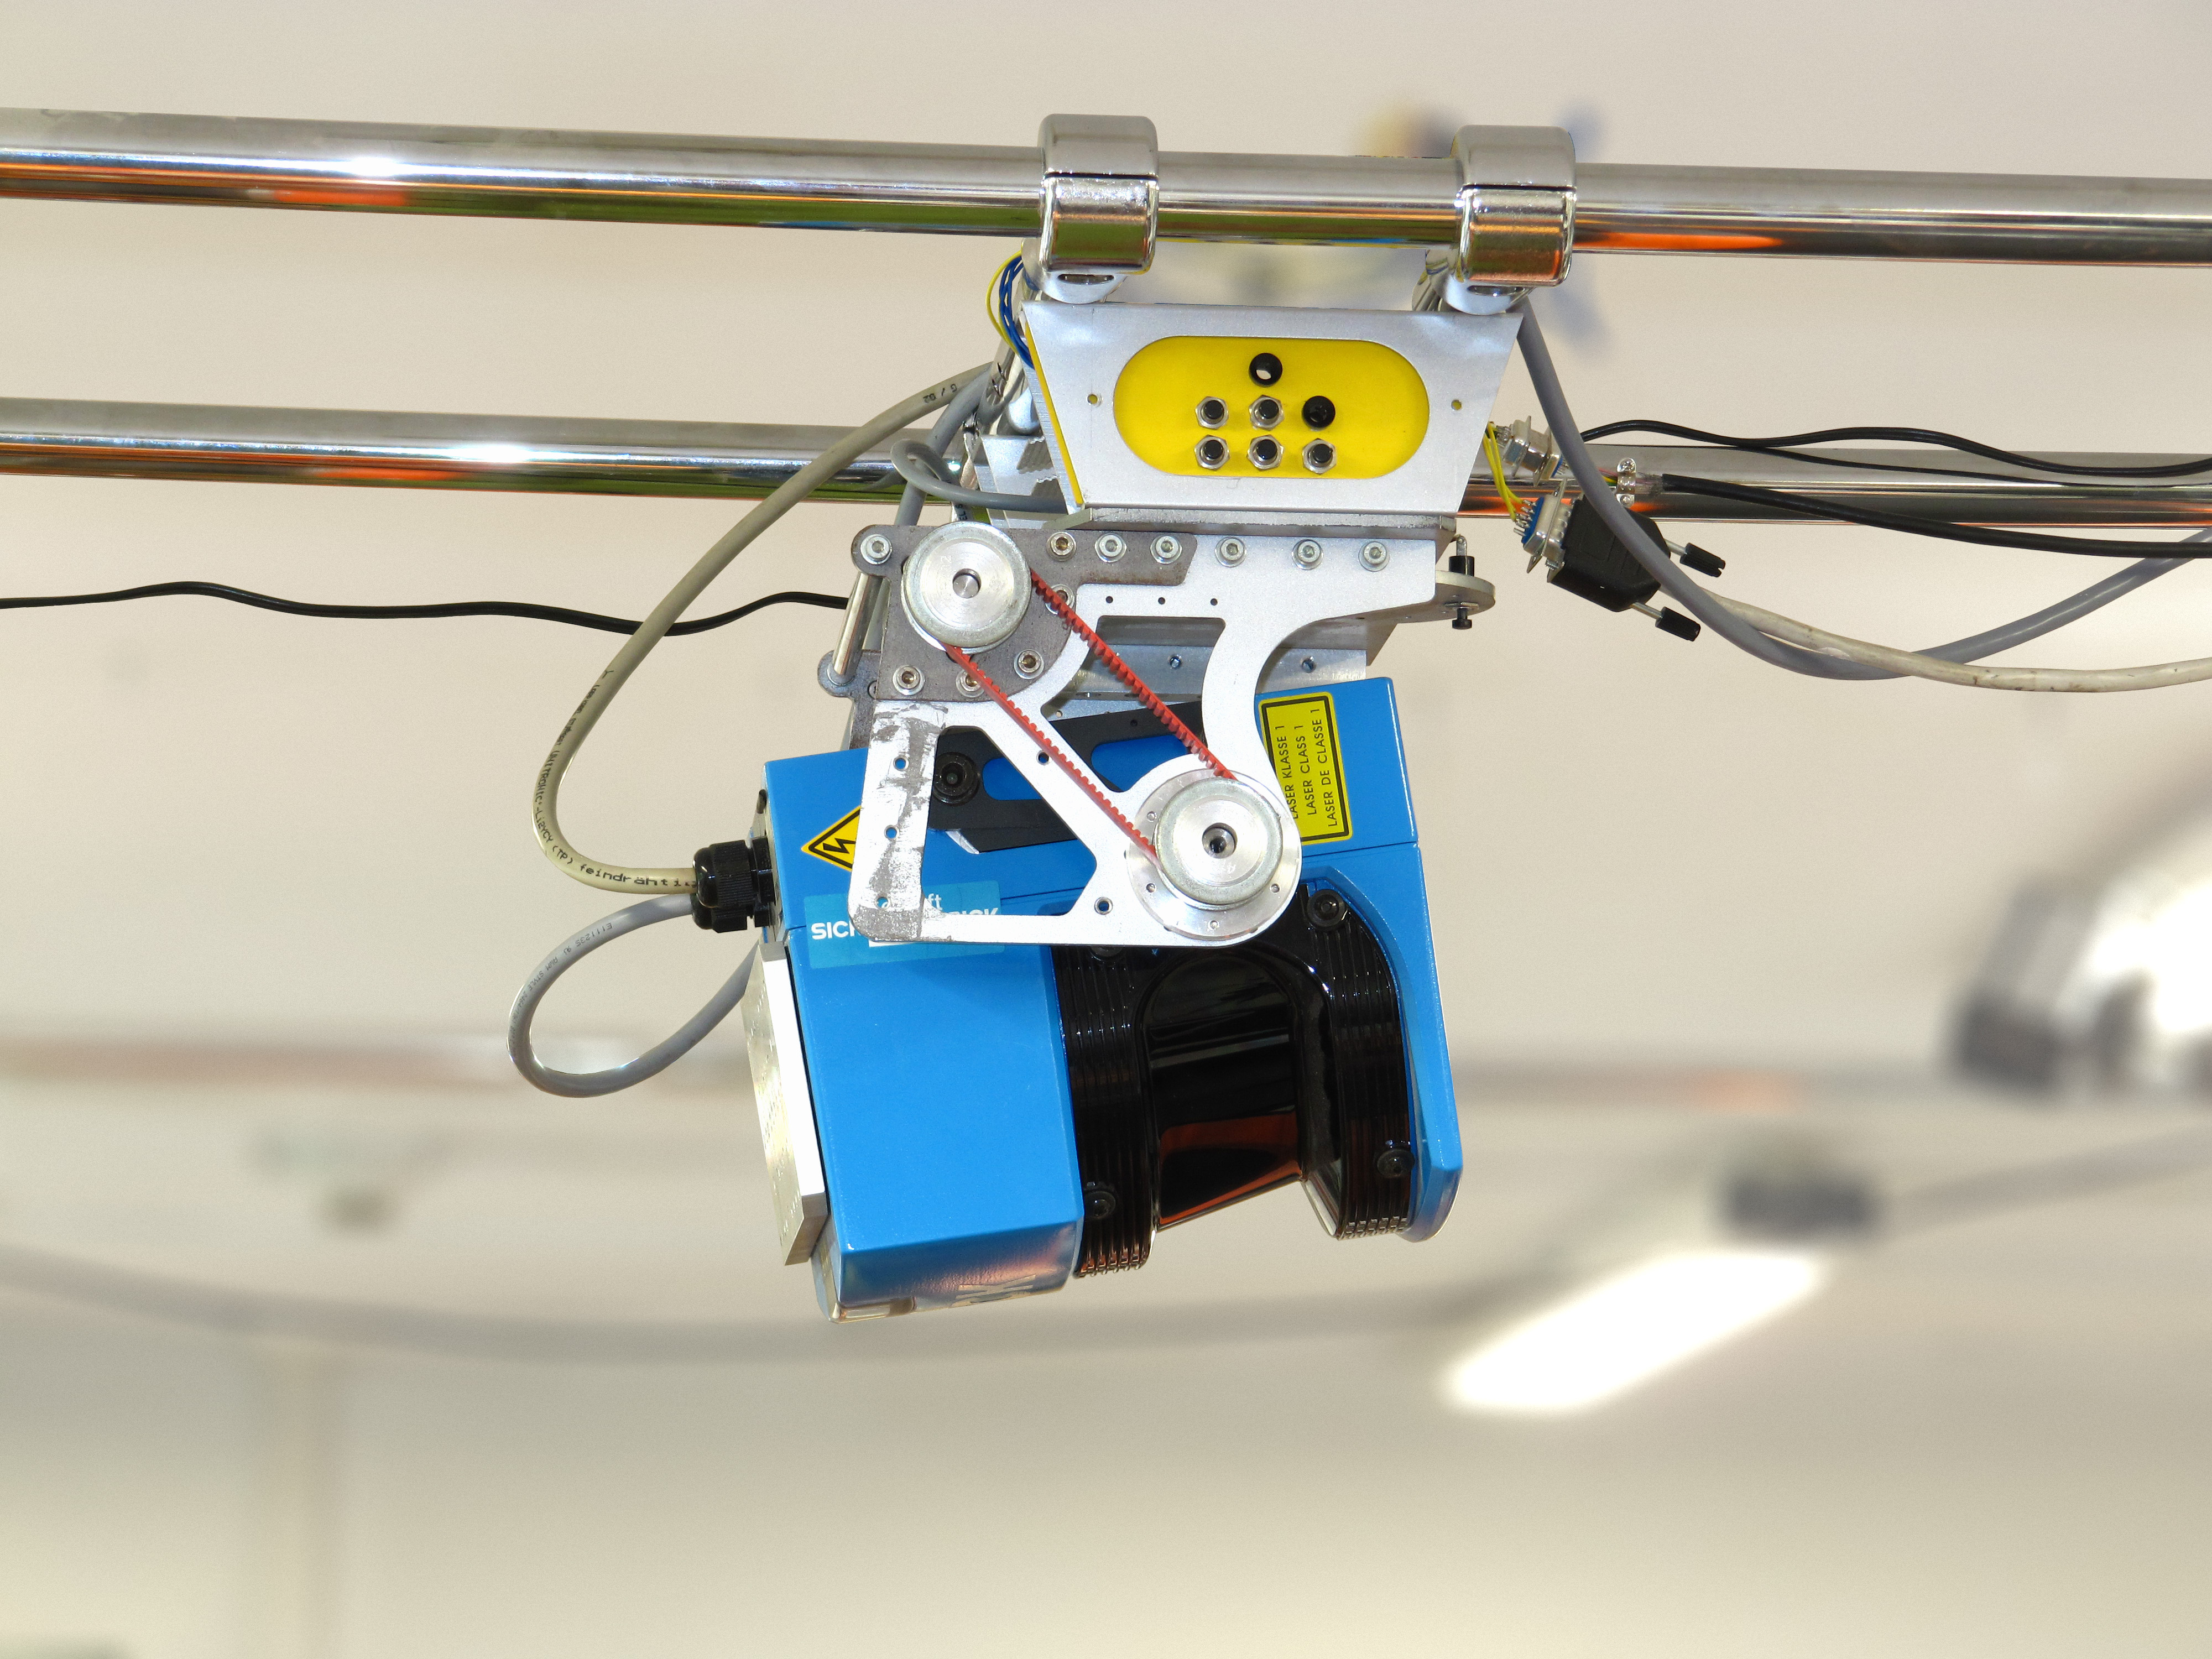
\includegraphics[height=6cm]{../../Common/img/sick_obrotnica} 
\caption{Skaner laserowy Sick LMS200 zamocowany na obrotnicy}
\label{fig:sick_obrotnica}
\end{figure}

\subsection{Sposoby interpolacji map głębi} 

Najprostszym sposobem wykorzystania uzyskiwanej informacji jest zapisanie
uzyskiwanych wyników wprost w mapie głębi. Można jednak wykorzystać fakt, że
skany wykonywane są w pewnych określonych sekwencjach, głównie liniami. Dzięki
temu w trakcie zbierania kolejnych pomiarów można dokonywać od razu
interpretacji i przetwarzania tych danych w celu stworzenia innej reprezentacji
otoczenia. W każdej kolejnej zeskanowanej linii można wyszukiwać za pomocą
odpowiednich algorytmów odcinki proste, a te zebrane w kolejnych skanach mogą
byc składane w większe płaszczyzny. Obliczenia te wykonywane są w tym samym
czasie, co zbieranie pomiarów, dzięki czemu praktycznie od razu po wykonaniu
ostatniego skanu dostajemy oprócz samej mapy głębi dodatkowe informacje o
geometrii sceny. Kolejne etapy opisanej agregacji danych
pokazane są na rysunku~\ref{fig:laser_aggregate}~\cite{Surmann01a3d}.

\begin{figure}[h!]
\centering
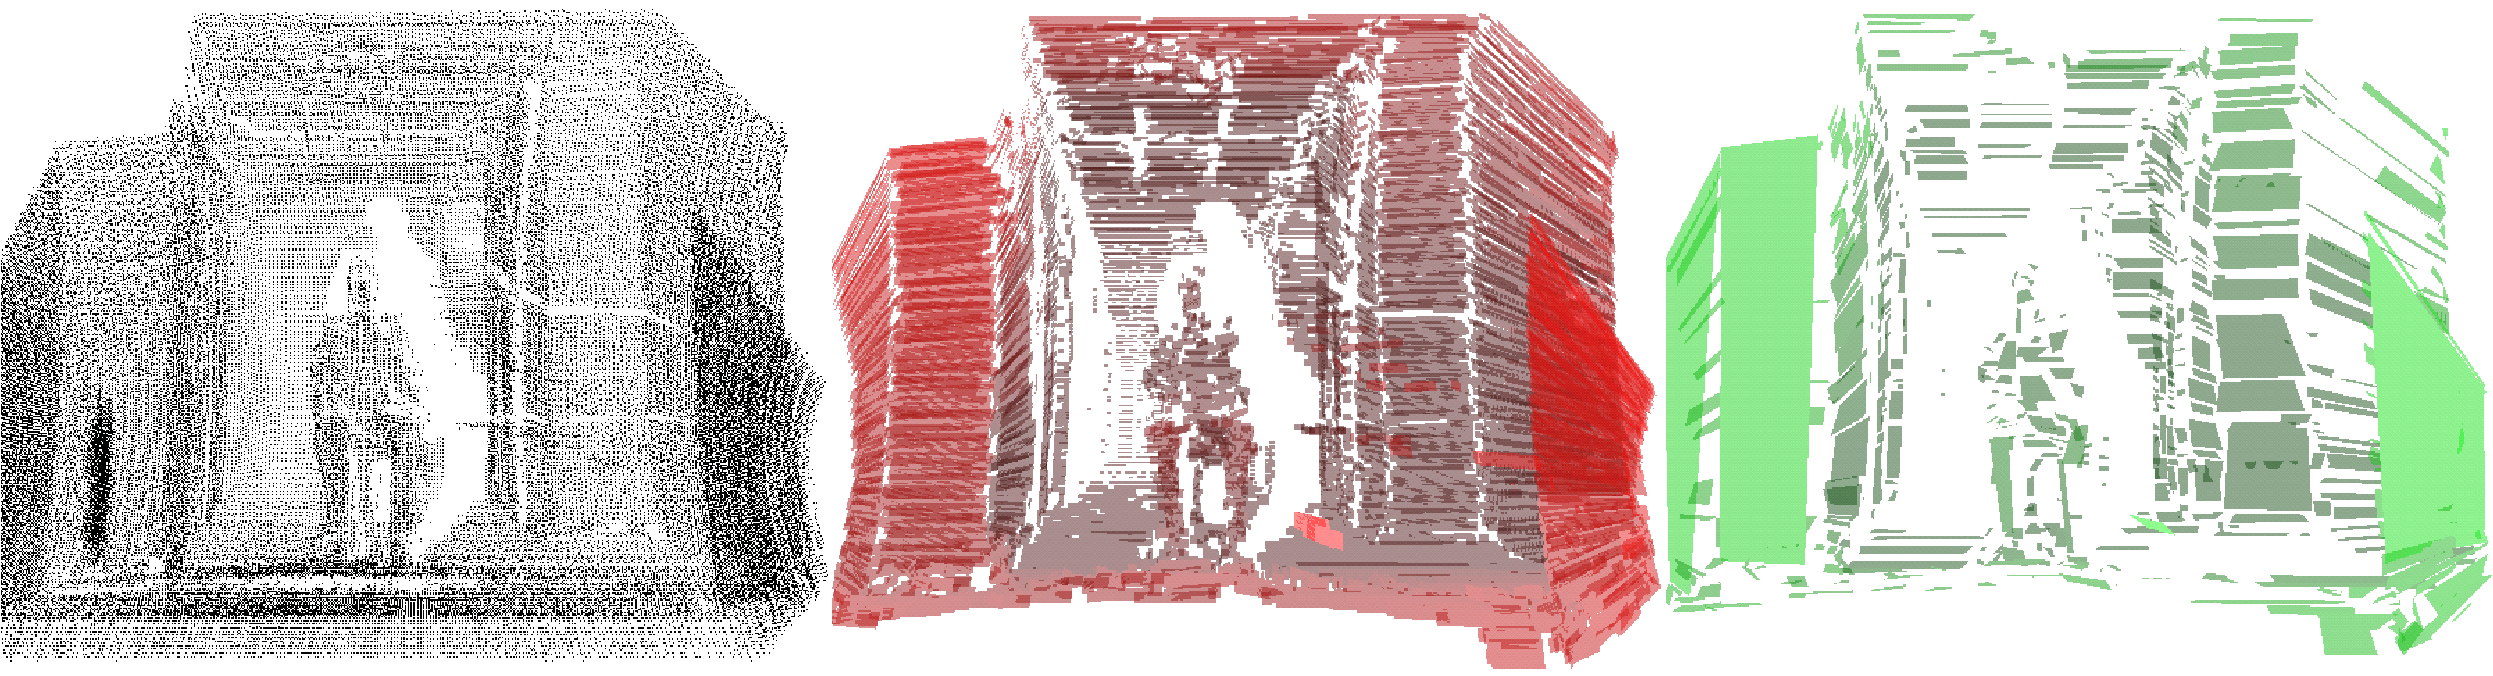
\includegraphics[width=12cm]{../../Common/img/laser_aggregate} 
\caption{Kolejne poziomy agregacji danych zebranych przy pomocy skanera
laserowego}
\label{fig:laser_aggregate}
\end{figure}

%%%%%%%%%%%%%%%%%%%%%%%%%%%%%%%%%%%%%%%%%%%%%%%%%%%%%%%%%%%%%%%%%%%%%%%%%%%%%%%%
%%%%%%%%%%%%%%%%%%%%%%%%%%%%%%%%%%%%%%%%%%%%%%%%%%%%%%%%%%%%%%%%%%%%%%%%%%%%%%%%
\section{Stereowizja}
%%%%%%%%%%%%%%%%%%%%%%%%%%%%%%%%%%%%%%%%%%%%%%%%%%%%%%%%%%%%%%%%%%%%%%%%%%%%%%%%
%%%%%%%%%%%%%%%%%%%%%%%%%%%%%%%%%%%%%%%%%%%%%%%%%%%%%%%%%%%%%%%%%%%%%%%%%%%%%%%%

%-------------------------------------------------------------------------------
\subsection{Zasada działania}
%-------------------------------------------------------------------------------

Stereowizja jest techniką obrazowania opierającą się na analizie obrazów wielu
(najczęściej dwóch) kamer. Algorytmy bazują na dysparacji, czyli względnej
odległości pomiędzy obrazami tego samego punktu w różnych kamerach, można w
nich wydzielić 3 kroki:

\begin{enumerate}
\item detekcja punktów charakterystycznych
\item dopasowanie odpowiedników
\item rekonstrukcja współrzędnych 3D
\end{enumerate}

Rysunek~\ref{fig:epipolar} przedstawia poglądowo zasadę działania algorytmów
stereowizyjnych. Rzeczywiste punkty $X$, $X_1$, $X_2$ oraz $X_3$ są współliniowe
względem lewej kamery (widoczne w obrazie jako ten sam punkt $X_L$). W obrazie z
prawej kamery punkty te są już rozróżnialne (punkt $X$ jest widoczny jako punkt
$X_R$). Znając współrzędne środków optycznych ($O_L$, $O_R$) i orientacje obu
kamer można wyznaczyć współrzędne linii epipolarnych dla badanych punktów, a
także rzeczywiste współrzędne tych punktów (na podstawie ich współrzędnych w
obu obrazach). W stereowizji najczęściej kamery ustawia się tak, aby ich osie
optyczne były możliwie równoległe, dzięki czemu łatwo wyznacza się linie
epipolarne (są poziome w obrazie) oraz odpowiednie punkty charakterystyczne.

\begin{figure}[h!]
\centering
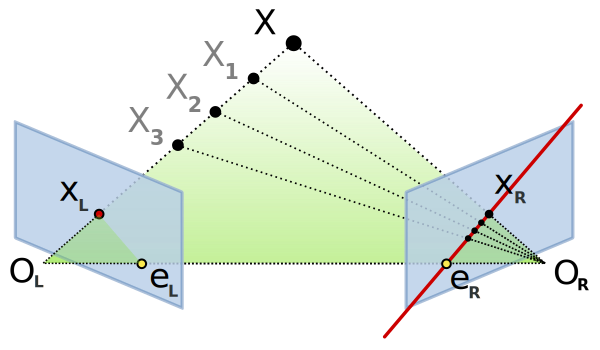
\includegraphics[width=8cm]{../../Common/img/Epipolar_geometry} 
\caption{Geometria dwubiegunowa}
\label{fig:epipolar}
\end{figure}

Dodatkowo konieczne jest wstępne przetworzenie obrazów tak, aby przedstawiały
one widok w taki sposób, jakby płaszczyzny obrazowania kamer były równoległe
(proces ten zwany jest rektyfikacją obrazu). W tym celu konieczna jest wstępna
kalibracja układu kamer, dająca w wyniku położenie kamer względem siebie
(przesunięcie oraz obrót), a także wyliczająca parametry wewnętrzne każdej z
kamer (zniekształcenia wnoszone przez soczewki obiektywu). Proces kalibracji
przeprowadza się raz dla danego położenia kamer, po każdorazowej zmianie ich
pozycji konieczna jest powtórna kalibracja. Rysunek~\ref{fig:stereo_steps}
przedstawia koleejne kroki podczas odtwarzania informacji o głębi z dwóch kamer.

\begin{figure}[h!]
\centering
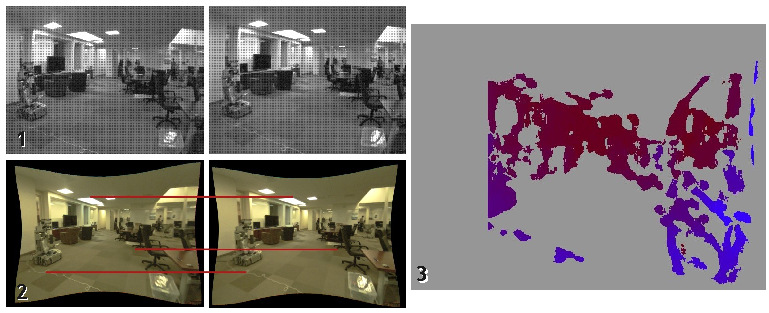
\includegraphics{../../Common/img/stereo_steps} 
\caption[Kolejne kroki podczas przetwarzania w stereowizji]
{Kolejne kroki podczas przetwarzania w stereowizji. 1: obraz pobrany
bezpośrednio z kamer; 2: obraz po interpolacji kolorów i rektyfikacji,
zaznaczone są także przykładowe, dopasowane punkty charakterystyczne; 3:
wynikowa mapa głebi dla podanej sceny.}
\label{fig:stereo_steps}
\end{figure}

%-------------------------------------------------------------------------------
\subsection{Wymagania sprzętowe}
%-------------------------------------------------------------------------------

Najważniejszym elementem przy stereowizji są kamery -- uzyskane rezultaty zależą
bezpośrednio od ich jakości. Stosowanie kamer z interfejsem analogowym jest
możliwe, jednak nie jest zalecane przy dynamicznych scenach. Obiekty
poruszające się z dużą szybkością są wykrywane błędnie bądź całkowicie
ignorowane ze względu na występujące rozmycie wynikające ze stosowania
przeplotu podczas akwizycji z kamer analogowych. Najlepsze wyniki uzyskuje się
stosując dobrej jakości kamery z interfejsami cyfrowymi, jednak ich koszt jest
dużo wyższy.

Samo rozmieszczenie kamer również ma istotny wpływ na uzyskiwane wyniki --
kamery umieszczone blisko siebie będą dawały dobre wyniki dla obiektów
znajdujących się blisko nich, kamery rozmieszczone szerzej pozwalają na
uzyskanie lepszej rozdzielczości dla obiektów znajdujących się daleko kosztem
częściowej bądź całkowitej utraty informacji o obiektach bliskich. Od
rozdzielczości kamery zależy uzyskiwana rozdzielczość przy rekonstrukcji sceny
3D, jednak wraz z jej wzrostem rośnie czas wymagany do przetworzenia
pojedynczej klatki obrazu.

\begin{figure}[h!]
\centering
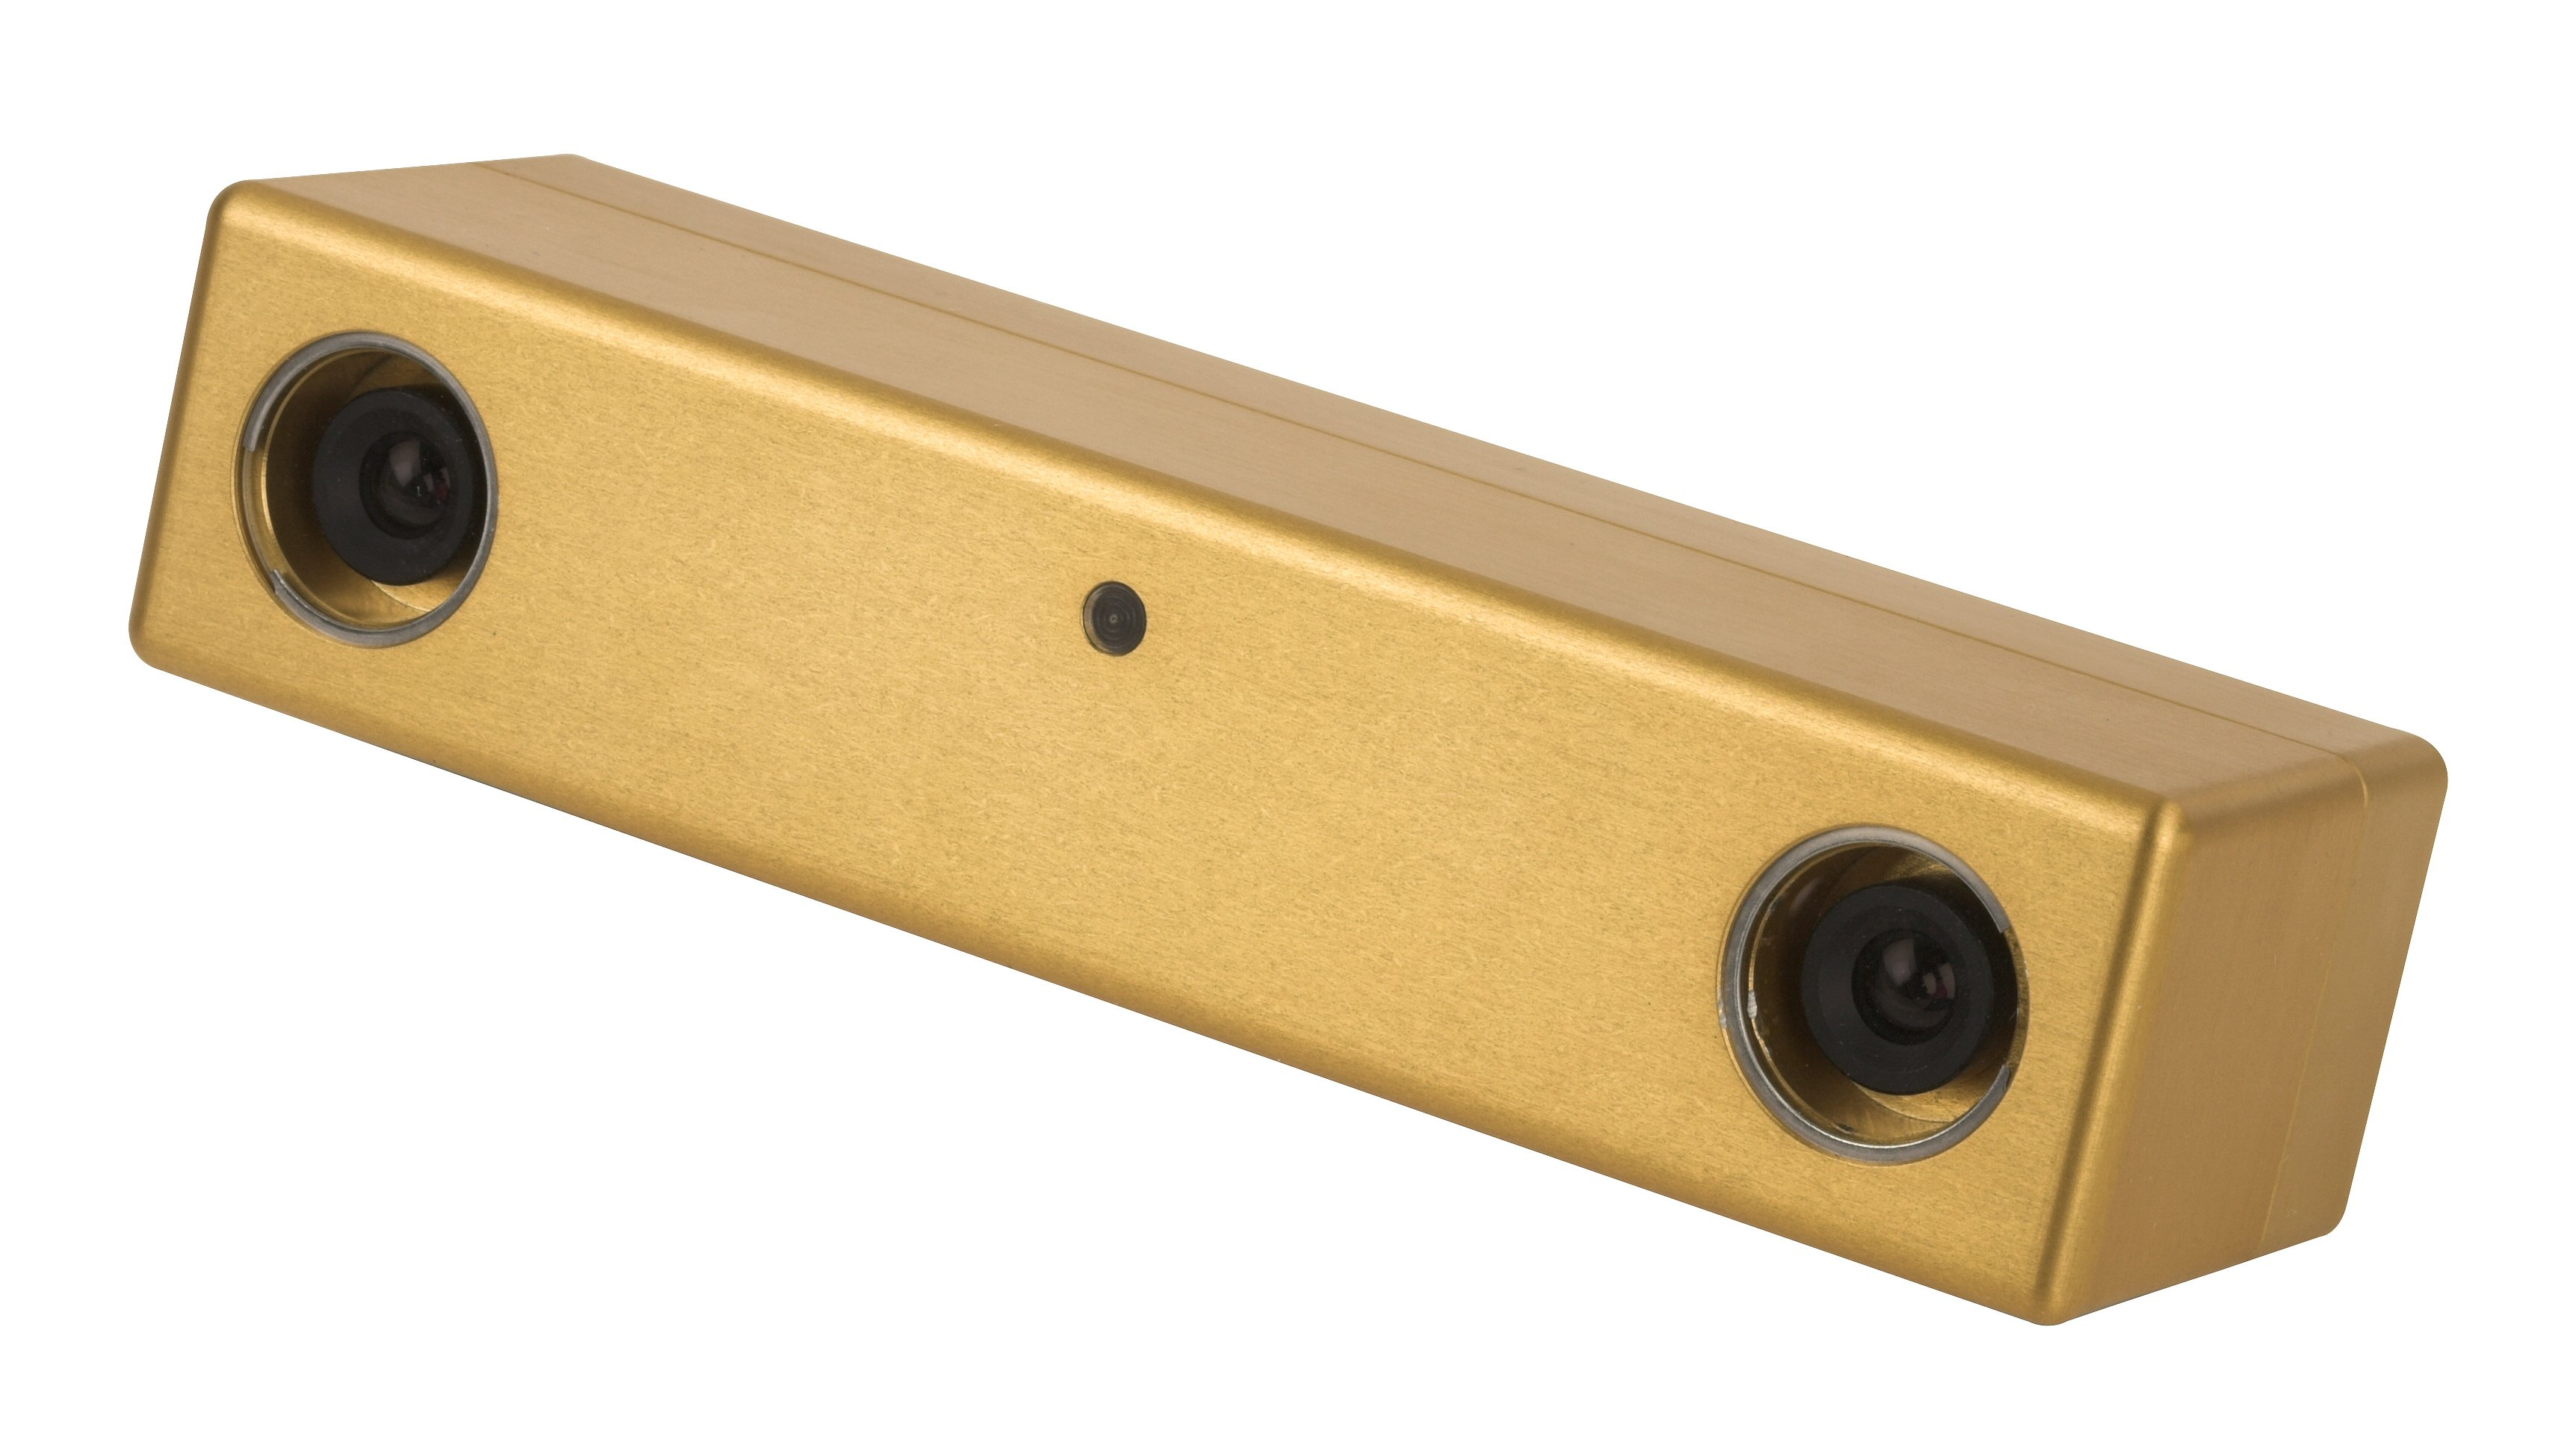
\includegraphics[width=8cm]{../../Common/img/bumblebee} 
\caption{Kamera do stereowizji Bumblebee X2}
\label{fig:bumblebee}
\end{figure}

Problemem może być samo mechaniczne mocowanie kamer. Musi być ono wykonane
bardzo solidnie, gdyż w przypadku nawet małej zmiany orientacji kamer względem
siebiewymagana jest ponowna kalibracja całego systemu. Aby pozbyć się tej wady
można stosować zintegrowane moduły zawierające dwie (bądź więcej) kamery w
jednej obudowie, to jednak uniemożliwia eksperymentowanie z odległością kamer
od siebie (patrz rysunek~\ref{fig:bumblebee}).

%-------------------------------------------------------------------------------
\subsection{Złożoność obliczeń}
%-------------------------------------------------------------------------------

% TODO: wstawić odwołania w odpowiednie miejsca
\cite{4670774} \cite{Hirschmuller:2008:SPS:1340087.1340245}

Przy wykorzystaniu programowej wersji algorytmów stereowizyjnych działających
na przeciętnym komputerze domowym, można osiągnąć wydajność od kilku do
kilkunastu klatek na sekundę. W związku z tym rozwiązania programowe słabo
nadają się do wykorzystania w środowisku, które ulega częstym i dynamicznym
zmianom (a takie jest otoczenie robota mobilnego).

Dużo lepiej sprawdzają się rozwiązania sprzętowe, w których algorytm tworzenia
mapy dysparacji zaimplementowany jest w układach FPGA zintegrowanych w jednym
module z kamerami. W tym przypadku wydajność jest stała i niezależna od platformy,
na której uruchomione będą algorytmy sterowania robota, i wynosi (w zależności
od producenta) od kilkunastu do ponad 30 FPS. Największą wadą takiego rozwiązania
jest jego koszt -- wynoszący od kilkuset do kilku tysięcy dolarów. Dla porównania
dwie kamery analogowe można kupić za ok. 200\$.

%-------------------------------------------------------------------------------
\subsection{Zastosowania}
%-------------------------------------------------------------------------------

Algorytm opiera się o wykrywanie punktów charakterystycznych w obrazie, a to
najczęściej sprowadza się do analizy obrazu krawędziowego. W związku z tym
obiekty o jednolitej, drobnej teksturze (bądź całkowicie gładkie) są słabo bądź
całkowicie niewykrywalne. W najlepszym wypadku wykrywane są jedynie ich
krawędzie, co prowadzi do powstawania dużych, niezidentyfikowanych obszarów w
obrazie (rysunek~\ref{fig:stereo_3} przedstawia taką sytuację).

Jednym z rozwiązań tego problemu może być zastosowanie dodatkowego projektora
wyświetlającego specjalnie przygotowany wzór (przykład na
rysunku~\ref{fig:stereo_texture}) w celu pokrycia obiektów sztuczną teksturą
umożliwiającą poprawę wyników stereowizji. Drugą możlwością poprawy sytuacji
jest stosowanie dodatkowego etapu przetwarzania obrazu po wygenerowaniu
wstępnej mapy głębokości. Po segmentacji obrazu na podstawie koloru wybierane
są obszary jednolite, a następnie w mapie głębi wypełniane są interpolowanymi
wartościami z ich krawędzi.

\begin{figure}[htpb!]
\centering
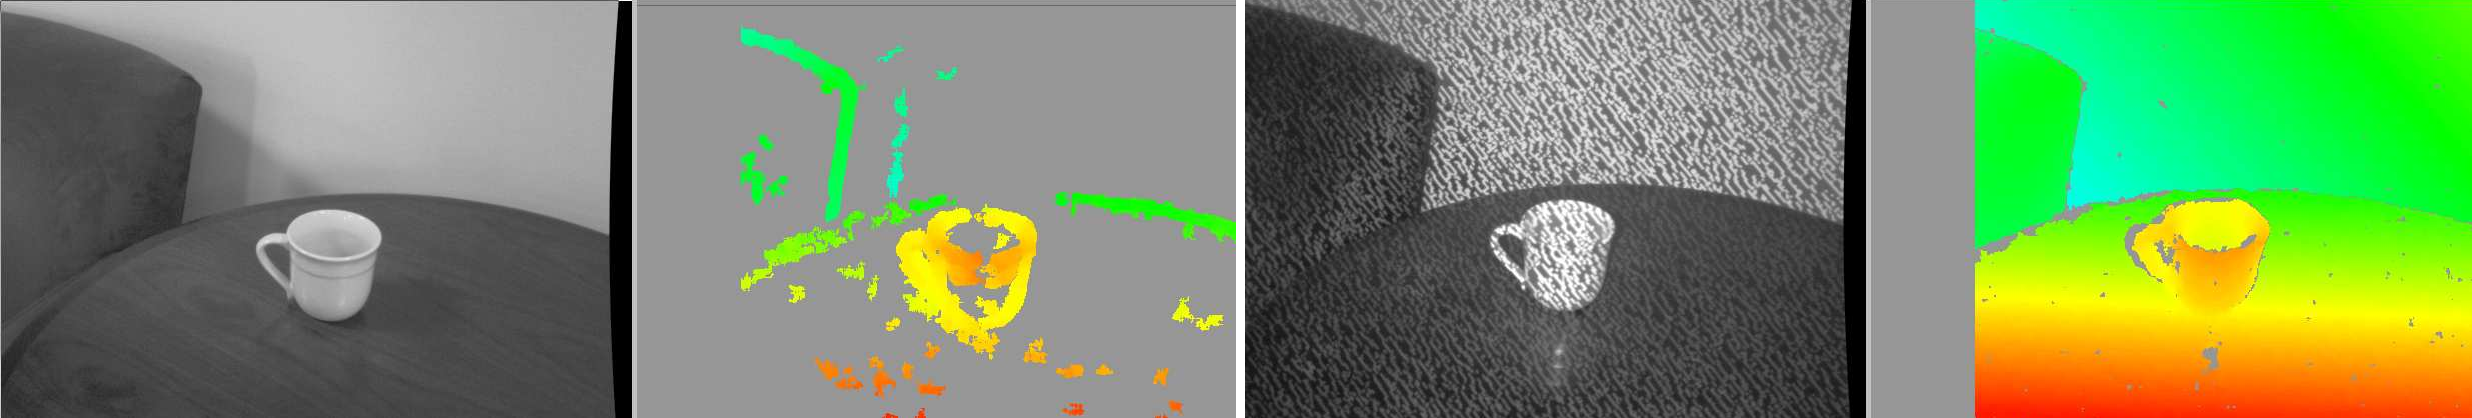
\includegraphics[width=16cm]{../../Common/img/stereo_texture} 
\caption[Przykład projekcji tekstury w celu poprawy jakości
stereowizji]{Przykład projekcji tekstury w celu poprawy jakości stereowizji
\cite{konolige-icra-2010-a} W kolejności od lewej: scena bez dodatkowego
oświetlenia, wygenerowana mapa głębi, scena z rzutowaną teksturą, poprawiona
mapa głębi}
\label{fig:stereo_texture}
\end{figure}

Oba rozwiązania dają dobre rezultaty, jednak komplikują bądź budowę urządzenia,
bądź wprowadzają dodatkowy narzut obliczeniowy. Projekcja tekstury bywa
z powodzeniem wykorzystywana w robotach mobilnych \cite{piorkowski2008}, a
bardziej skomplikowane algorytmy stosowane są na dużych robotach
manipulacyjno-przemysłowych, które są wyposażone w odpowiednio wydajne
jednostki obliczeniowe (np. robot PR2). Natomiast w robotach poruszających się
w naturalnym środowisku, gdzie występuje bardzo dużo szczegółów (a więc i
punktów charakterystycznych) stereowizja stosowana jest praktycznie bez żadnych
dodatkowych usprawnień i sprawdza się znakomicie (zwracane mapy głębi są
wypełnione w ponad 80\%, a algorytm działa w tempie powyżej 10FPS)
\cite{outdoor-stereo}.


%%%%%%%%%%%%%%%%%%%%%%%%%%%%%%%%%%%%%%%%%%%%%%%%%%%%%%%%%%%%%%%%%%%%%%%%%%%%%%%%
%%%%%%%%%%%%%%%%%%%%%%%%%%%%%%%%%%%%%%%%%%%%%%%%%%%%%%%%%%%%%%%%%%%%%%%%%%%%%%%%
\section{Światło strukturalne}
%%%%%%%%%%%%%%%%%%%%%%%%%%%%%%%%%%%%%%%%%%%%%%%%%%%%%%%%%%%%%%%%%%%%%%%%%%%%%%%%
%%%%%%%%%%%%%%%%%%%%%%%%%%%%%%%%%%%%%%%%%%%%%%%%%%%%%%%%%%%%%%%%%%%%%%%%%%%%%%%%

%-------------------------------------------------------------------------------
\subsection{Zasada działania}
%-------------------------------------------------------------------------------

Inną metodą pomiaru i odtwarzania informacji i głębi sceny bazującą na analizie
obrazu jest wykorzystanie światła strukturalnego. Na scenę rzucane jest światło
formujące znany wzór, a kamera umieszczona jest w taki sposób, aby obserwować
scenę pod innym kątem niż orientacja rzutnika. Na podstawie odczytanej deformacji
wzorca prz użyciu algorytmów bazujących na riangulacji wyliczane są rzeczywiste
współrzędne punktów w obrazie. 

\begin{figure}[htb!]
\centering
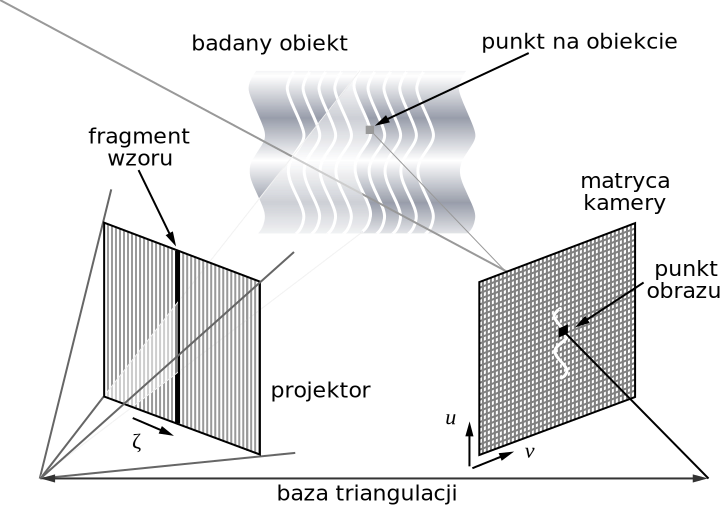
\includegraphics[width=10cm]{../../Common/img/struct} 
\caption[Schemat działania skanera opartego o światło strukturalne]
{Schemat działania skanera opartego o światło strukturalne. Na podstawie:
http://en.wikipedia.org/wiki/File:1-stripesx7.svg}
\label{fig:struct_principle}
\end{figure}

Rzutowane mogą być różne wzory, zaczynając od pojedynczego punktu, przez
wzory złożone z linii (statycznych bądź przesuwających się po
scenie, w takim przypadku scena jest analizowana stopniowo), aż po złożone,
pseudoloswe wzory (także kolorowe) oraz sekwencje wzorów \cite{1588327}. W
przypadku korzystania z sekwencji wzorów wymagany jest statyczny charakter
sceny, sceny dynamiczne wymagają stosowania pojedynczych, skomplikowanych
struktur.

\begin{figure}[h!]
\centering
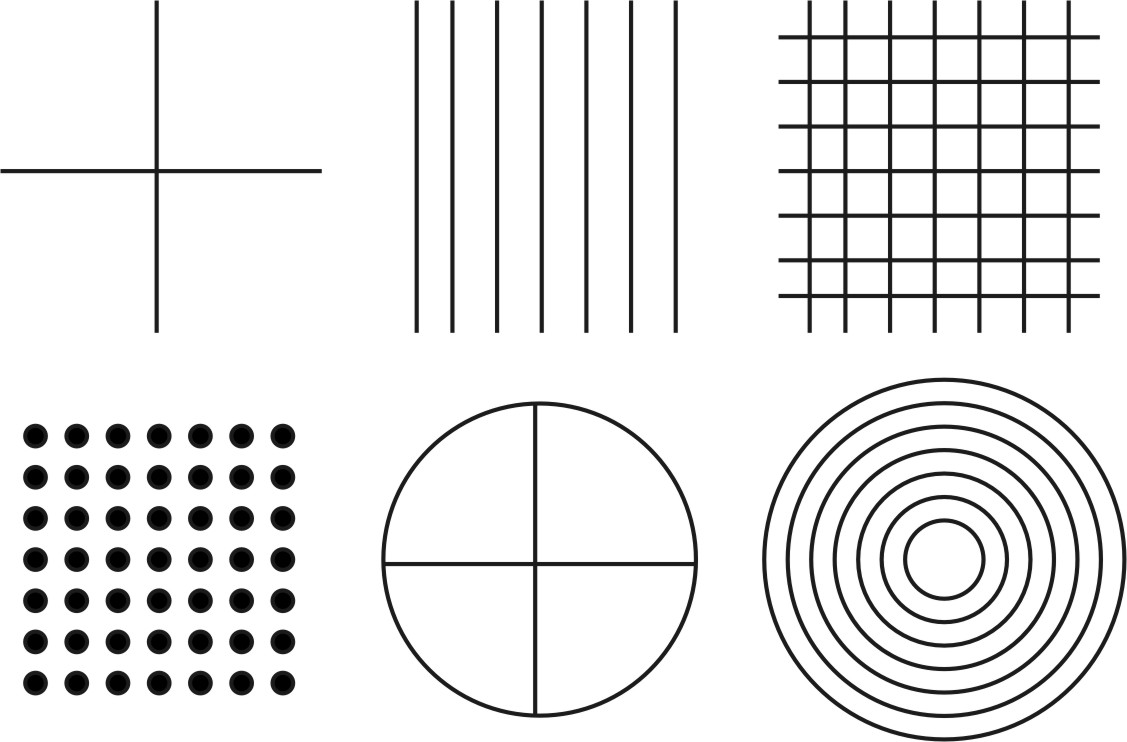
\includegraphics[width=8cm]{../../Common/img/struct_patterns} 
\caption[Wzorce wykorzystywane przy obrazowaniu światłem strukturalnym]
{Wzorce wykorzystywane przy obrazowaniu światłem strukturalnym}
\label{fig:struct_patterns}
\end{figure}

%-------------------------------------------------------------------------------
\subsection{Zastosowania}
%-------------------------------------------------------------------------------

Głównym kryterium przy wyborze konkretnej realizacji skanera opartego o światło
strukturalne jest charakter analizowanej sceny. W przypadku skanowania obiektów
statycznych (np. podczas automatycznego tworzenia modeli trójwymiarowych)
możliwe jest zastosowanie sekwencji wzorców, np. kodu Graya. Stosowane są też
różne rozwiązania pomocnicze w celu zeskanowania obiektu ze wszystkich stron bez
jego obracania (np. zestaw specjalnie ustawionych luster) \cite{LanmanCT07}.

\begin{figure}[!ht]
\centering
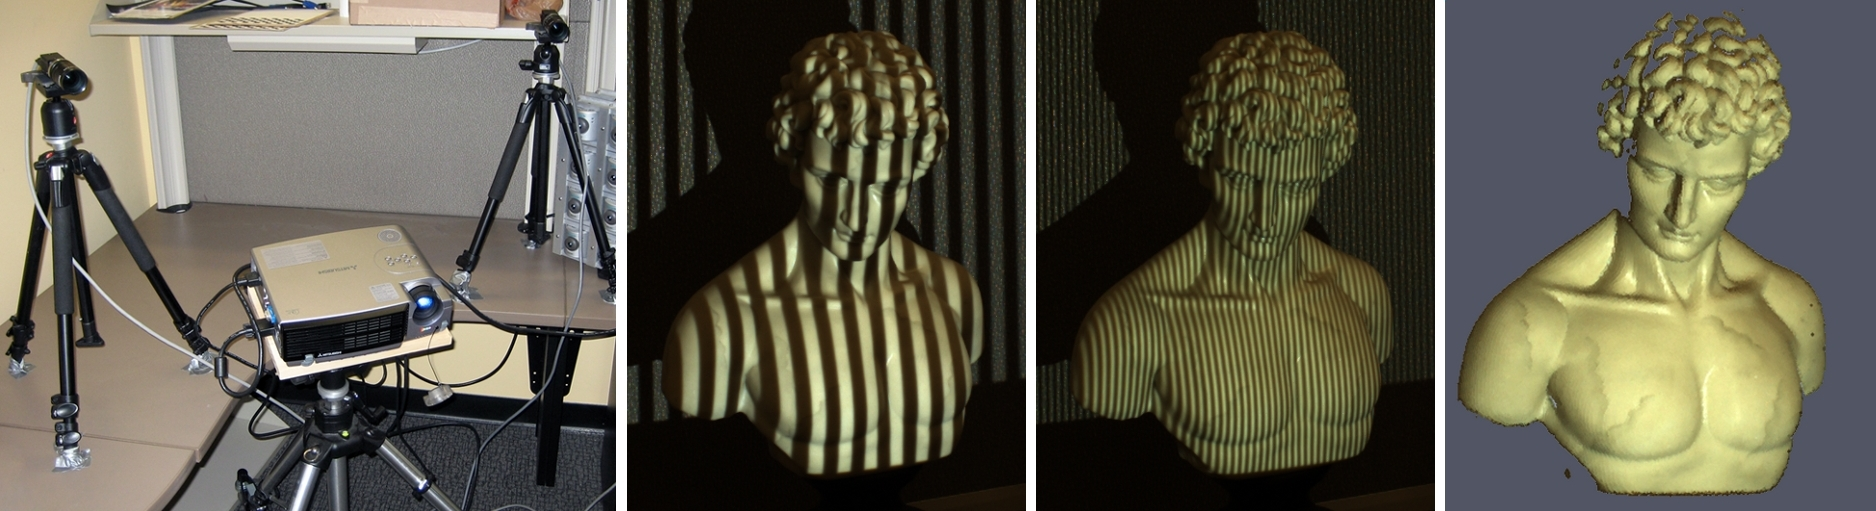
\includegraphics[width=14cm]{../../Common/img/struct_all} 
\caption[Przykład wykorzystania światła strukturalnego do modelowania obiektów]
{Przykład wykorzystania światła strukturalnego do modelowania obiektów. Na
pierwszym zdjęciu widać układ pomiarowy, następnie dwa wybrane etapy oświetlania
kodem Graya oraz wynikowy model otrzymany po oświetleniu 40-toma wzorcami.
Źródło: http://web.media.mit.edu/~dlanman/}
\label{fig:struct_all}
\end{figure}

Do zastosowań czasu rzeczywistego, jak już wspomniano wcześniej, nadają się
jedynie wzorce pojedyncze. Dzięki temu każda otrzymana klatka obrazu zawiera
informacje o całym modelu, w metodach opartych o wzorce sekwencyjne obiekt
przesuwający się pomiędzy kolejnymi naświetleniami powoduje zakłamanie wyników. 
Wśród takich metod wyróżnić można oparte o wzorce kodowane geometrycznie i
kolorowo. Pierwsza z metod wykorzystuje jednobarwne wzorce geometryczne
zakodowane w taki sposób, aby poszczególne jego bloki były unikalne w pewnym
otoczeniu. W przypadku tej drugiej metody stosowane są np. różnokolorowe pasy
bądź szachownice, a z układu kolorów rekonstruowana jest powierzchnia obiektów.
Rozwiązania te cechują się dużą szybkością działania, od kilkunastu do ponad
stu klatek przetwarzanych w ciągu sekundy \cite{4429304}.

\begin{figure}[h!]
\centering
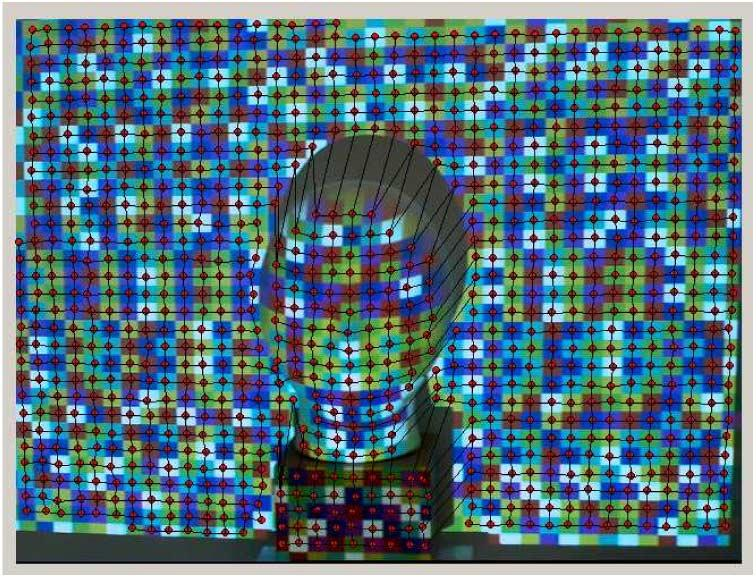
\includegraphics[width=8cm]{../../Common/img/struct_color} 
\caption[Wzorzec kodowany kolorem]
{Jedna z możliwości kolorowego kodowania wzorców \cite{4429304}}
\label{fig:struct_color}
\end{figure}

W zastosowaniach robotycznych, w przypadku, kiedy maszyny mają działać we
wspólnym otoczeniu z ludźmi, wzorce kodowane kolorami są niewygodne -- musza one
działać w paśmie światła widzialnego, co może przeszkadzać będącym w pobliżu
ludziom. W takim wypadkuz zdecydowanie lepiej sprawdzają się wzorce
geometryczne, których rzutniki mogą działać w podczerwieni, a więc w sposób
niewidoczny i nieprzeszkadzający użytkownikom. W taki właśnie sposób działa
Microsoft Kinect, opisany dokładnie w rozdziale~\ref{chap:sprzet}.  

Największą niedogodnością związaną z wykorzystaniem obrazowania opartego o
rzutowanie wzorców jest konieczność dokładnego wykrycia tego wzoru. Dlatego też
najczęściej stosowane jest ono na niewielkie odległości, przy skanowaniu
pojedynczych obiektów. Przy stosowaniu na większe odległości konieczne jest
stosowanie bądź projekcji w paśmie podczerwonym (aby wykluczyć zakłócenia od
tradycyjnych źródeł światła), bądź wykorzystanie projektorów o bardzo dużej
mocy. Żaden z wariantów nie sprawdza się jednak na otwartej przestrzeni, gdzie
światło słoneczne zakłóca działanie praktycznie wszystkich sensorów tego typu.

%-------------------------------------------------------------------------------
\subsection{Rozwiązania programowe i sprzętowe} 
%-------------------------------------------------------------------------------

W przypadku stosowania algorytmów zaimplementowanych programowo uruchamianych na
komputerze sterującym można wymienić praktycznie takie same wady, jak przy
stereowizji, Największą z nich jest obciążenie systemu, gdyż algorytm jest
dość skomplikowany. Rozwiązania sprzętowe rozwiązują problem szybkości działania
i obciążenia komputera sterującego, jednak ich cena przez bardzo długi czas
była wysoka (rzędu setek do tysięcy dolarów). Pod koniec 2010 roku pojawił się
na runku wspomniany wcześniej Microsoft Kinect -- urządzenie o cenie o
rząd wielkości niższej, będące faktycznie sprzętowym sensorem głębi opartym o
analizę światła strukturalnego. Niską cenę zawdzięcza masowej produkcji -- jest
produkowany jako kontroler do gier, i jako taki ma zdecydowanie większy rynek
zbytu niż tradycyjne, specjalizowane rozwiązania. 

Przed pojawieniem się na rynku urządzenia Microsoft Kinect, w robotyce mobilnej
stosowane były głównie rozwiązania oparte o obrazowanie na podstawie projekcji
pojedynczych linii (\cite{120445,5246792}), głównie ze względu na prostotę
koniecznych obliczeń i szybkość działania całego systemu. 


%%%%%%%%%%%%%%%%%%%%%%%%%%%%%%%%%%%%%%%%%%%%%%%%%%%%%%%%%%%%%%%%%%%%%%%%%%%%%%%%
%%%%%%%%%%%%%%%%%%%%%%%%%%%%%%%%%%%%%%%%%%%%%%%%%%%%%%%%%%%%%%%%%%%%%%%%%%%%%%%%
\section{Pomiar czasu przelotu wiązki światła}
%%%%%%%%%%%%%%%%%%%%%%%%%%%%%%%%%%%%%%%%%%%%%%%%%%%%%%%%%%%%%%%%%%%%%%%%%%%%%%%%
%%%%%%%%%%%%%%%%%%%%%%%%%%%%%%%%%%%%%%%%%%%%%%%%%%%%%%%%%%%%%%%%%%%%%%%%%%%%%%%%

Kamery TOF\footnote{z ang. {\it time-of-flight}, czas przelotu} działają na zasadzie
pomiaru czasu przelotu wiązki światła od projektora do kamery po jego odbiciu od
obiektów. Działanie to jest analogiczne do działania skanerów laserowych, z tą różnicą,
że w przypadku skanerów emitowana jest pojedyncza wiązka światła, natomiast kamery TOF
oświetlają i wykonują pomiar całej sceny naraz.

%-------------------------------------------------------------------------------
\subsection{Zasada działania i wykorzystanie}
%-------------------------------------------------------------------------------

Kamery TOF mogą działać w oparciu o dwie główne metody: bezpośredni pomiar
czasu przelotu wiązki światła (od błysku naświetlającego scenę do jego
zarejestrowania na matrycy) bądź pośredni pomiar tej wielkości z różnicy fazy
emitowanego światła (w tym przypadku bez przerwy emitowane jest modulowane
światło~\cite{910448}). W obu wypadkach wyliczony czas przelotu dla każdego
punktu zarejestrowanego obrazu jest proporcjonalny do jego odległości od kamery.

\begin{figure}[h!]
\centering
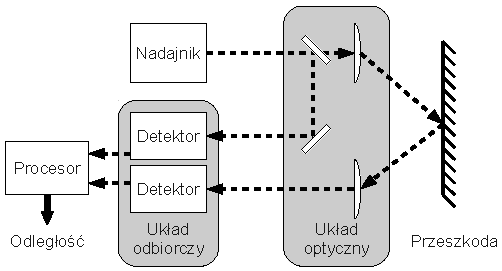
\includegraphics[width=8cm]{../../Common/img/tof} 
\caption{Schemat działania kamer TOF mierzących bezpośrednio czas przelotu}
\label{fig:tof}
\end{figure}

Kamery typu TOF są wykorzystywane w robotyce mobilnej głównie w robotach
operujących w pomieszczeniach~\cite{Prusak:2008:PEM:1462089.1462102}. Dokładność
uzyskiwanych pomiarów, szybkość działania i niskie obciążenie komputera
sterującego pozwalają na wykorzystanie otrzymywanego obrazu nie tylko do
wykrywania i omijania przeszkód, ale także do budowy mapy otoczenia i
samolokalizacji robota (na podstawie obserwacji punktów charakterystycznych w
mapie głębi). Sama technologia wykonania sensora sprawia jednak, że do
rejestracji obrazu kolorowego wymagana jest dodatkowa kamera, skalibrowana z
modułem głębi (niedogodność ta nie wystepuje przy stosowaniu stereowizji oraz
wielu metod opartych o analizę światła strukturalnego).

%-------------------------------------------------------------------------------
\subsection{Właściwości metody}
%-------------------------------------------------------------------------------

Zastosowanie metody opartej o pomiar czasu powrotu wiązki światła pozwala na
umieszczenie projektora i matrycy rejestrującej obraz bardzo blisko siebie (w
szczególności współosiowo, z diodami projektora umieszczonymi dookoła obiektywu
kamery), dzięki czemu nie występuje największa wada systemów opartych o
triangulację (stereowizja i światło strukturalne), czyli powstawanie cieni.
Spośród innych zalet tej metody pomiaru wymienić można chociażby zwartą
konstrukcję sensora (cały system składa się z pojedynczego modułu zawierającego
zarówno kamerę jak i oświetlacz), dzięki czemu jest on bardzo łatwy do
zastosowania w gotowym robocie. Nie bez znaczenia jest też szybkość działania --
dzięki naświetlaniu całej klatki jednocześnie oraz biorąc pod uwagę prędkość 
światła, możliwe jest uzyskanie prędkości nawet 100 klatek na sekundę, a dzięki
całkowicie sprzętowemu przetwarzaniu danych uzyskuje się bardzo niskie
obciążenie systemu -- kamera zwraca obraz zawierający bądź czas przelotu
światła, z którego w prosty sposób obliczyć można odległość, bądź od razu gotową
mapę głębi. Widać tutaj dużą przewagę nad innymi rozwiązaniami, gdzie wymagane
jest stosowanie skomplikowanych algorytmów w celu wyliczenia ostatecznej
odległości do obiektów.

\begin{figure}[h!]
\centering
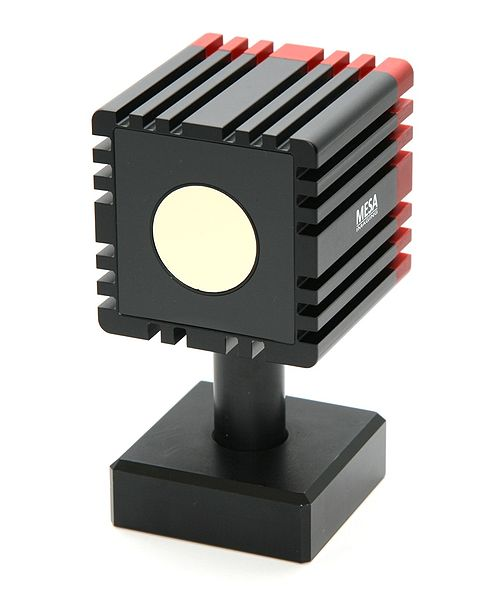
\includegraphics[height=5cm]{../../Common/img/sr4000} 
\caption[Kamera TOF SwissRanger SR4000]{Kamera TOF SwissRanger SR4000.
Rozdzielczość obrazu: 176x144px przy 54FPS, cena ok. 9000\$}
\label{fig:sr4000}
\end{figure}
 
Własności te sprawiają, że kamery TOF wydają się być bardzo dobrym rozwiązaniem
do zastosowania przy nawigacji robota. Niestety, mają też kilka wad, które to
wykorzystanie utrudniają. Pierwszą z nich jest cena -- jako że rozwiązania te są
stosunkowo nowe a także bardzo skomplikowane pod względem technicznym, ich cena
jest wielokrotnie wyższa od układów opartych na stereowizji lub świetle
strukturalnym. W porównaniu do tych metod niższa jest także rozdzielczość
uzyskiwanej mapy głębi -- obecnie produkowane sensory posiadają rozdzielczość
maksymalną rzędu 320x240px, a tańsze modele często posiadają rozdzielczość 
poniżej 100x100px. Sama technika wykonywania pomiaru ma kilka cech, które mogą
utrudniać jej wykorzystanie, np. występowanie wielokrotnych odbić, przez co
do sensora może dotrzeć i zostać zarejestrowane światło odbite i załamane od
obiektów znajdujących się bliżej, niż faktyczny punkt widziany w danym miejscu
matrycy. Podobnie zafałszowane pomiary mogą wystąpić przy obecności w
obserwowanej scenie silnych źródeł światła, praktycznie niemożliwe jest także
stosowanie tych metod w słoneczny dzień w terenie otwartym. Przy stosowaniu
wielu kamer TOF jednocześnie należy uwzględnić problem interferencji emitowanego
światła -- najczęściej rozwiązywany przez sekwencyjne odczyty z kolejnych kamer
(co z kolei zmniejsza faktyczną szybkość akwizycji danych).

\begin{figure}[h!]
\centering
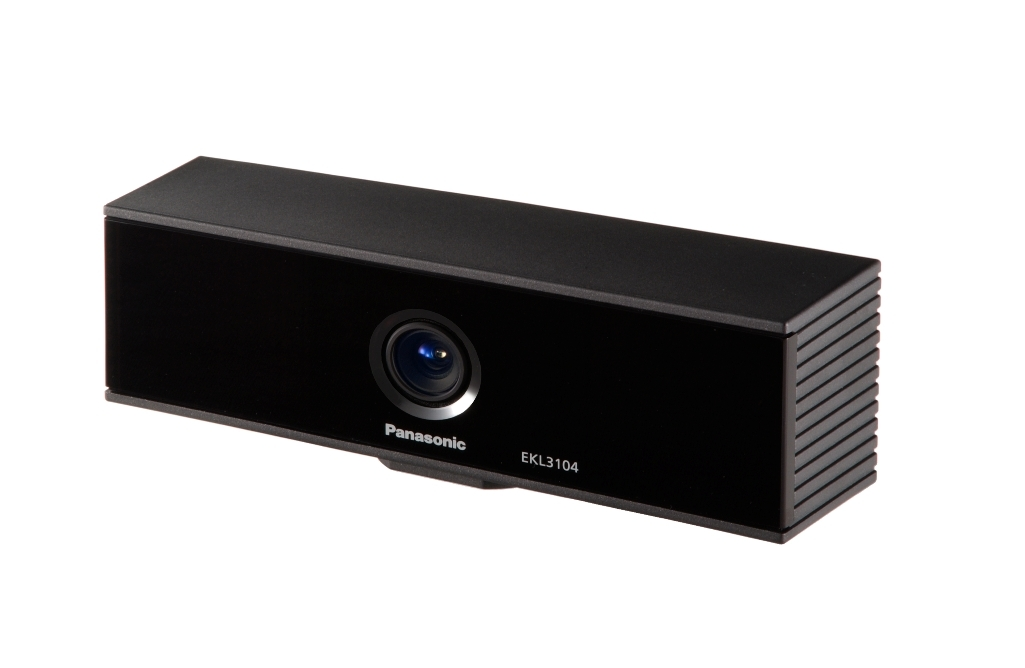
\includegraphics[height=5cm]{../../Common/img/dimager} 
\caption[Kamera TOF Panasonic D-IMager]{Kamera TOF Panasonic D-IMager.
Rozdzielczość obrazu: 160x120px przy 20FPS, cena ok. 3000\$}
\label{fig:dimager}
\end{figure}

%%%%%%%%%%%%%%%%%%%%%%%%%%%%%%%%%%%%%%%%%%%%%%%%%%%%%%%%%%%%%%%%%%%%%%%%%%%%%%%%
%%%%%%%%%%%%%%%%%%%%%%%%%%%%%%%%%%%%%%%%%%%%%%%%%%%%%%%%%%%%%%%%%%%%%%%%%%%%%%%%
\section{Porównanie dostępnych rozwiązań}
%%%%%%%%%%%%%%%%%%%%%%%%%%%%%%%%%%%%%%%%%%%%%%%%%%%%%%%%%%%%%%%%%%%%%%%%%%%%%%%%
%%%%%%%%%%%%%%%%%%%%%%%%%%%%%%%%%%%%%%%%%%%%%%%%%%%%%%%%%%%%%%%%%%%%%%%%%%%%%%%%

Ta część ma na celu porównanie dwóch dostępnych dla autora pracy rozwiązań --
stereowizji dwukamerowej i światła strukturalnego (sensora Microsoft Kinect).
Celem testów jest porównanie szybkości działania, obciążenia systemu i pokrycia
mapy głębi. Dokładność odwzorowania mapy głębi nie była obiektem testów, dlatego
wygenerowane mapy głębi mają różniące się skale kolorystyczne.

%-------------------------------------------------------------------------------
\subsection{Stereowizja -- Global Block Matching}
%-------------------------------------------------------------------------------

W celu sprawdzenia w praktyce jakie rezultaty można osiągnąć na dostępnym sprzęcie
przygotowano prosty układ pomiarowy i zebrano kilka pomiarów dla różnych scen.
Para stereowizyjna została złożona z dwóch kamer firmy Ganz, model ZC-NAF27, które
ustawione zostały w taki sposób, aby ich osie optyczne były możliwie równoległe,
a ich odległość wynosiła 12cm (podytkowane właściwościami mechanicznymi platformy,
na której zostały zamontowane). Po kalibracji obu kamer uruchomiono algorytm
dopasowania i generacji mapy dysparacji (wykorzystujący bibliotekę OpenCV) na
komputerze wyposażonym w procesor Intel Core2Duo E6550 2.33GHz oraz 4GB pamięci
RAM, pracującym pod kontrolą systemu Ubuntu 10.04. Wygenerowanie pojedynczej mapy
głębi zajmowało ok. 130ms (7.7 klatki na sekundę).

Poniżej przedstawione są wygenerowane mapy głębi nałożone na obraz z którego powstały
(dokładnie na obraz z lewej kamery, ponieważ w jej układzie mapa ta jest wyliczana).
Przedstawione są trzy sceny przedstawiające charakterystyczne cechy tej metody
pozyskiwania informacji o głebi. Scena przedstawiona na rysunku~\ref{fig:stereo_1}
zawiera dwie jednakowe przeszkody umieszczone w różnej odległości przed robotem.
Algorytm dobrze wykrywa krawędzie przeszkód, jednak na ich powierzchni oznaczane
są jedynie miejsca, gdzie naniesione są napisy i rysunki. W niektórych miejscach
widać błędne dopasowania punktów charakterystycznych (widoczne jako plama w kolorze
znacznie odbiegającym od otoczenia, np. na dole prawego pudełka). Szary kolor na
mapie głębi oznacza piksele niezidentyfikowane. Kolor piksela oznacza jego odległość
od kamery, najbliższe są czerwone, najdalsze są niebieskie.

\begin{figure}[h!]
\centering
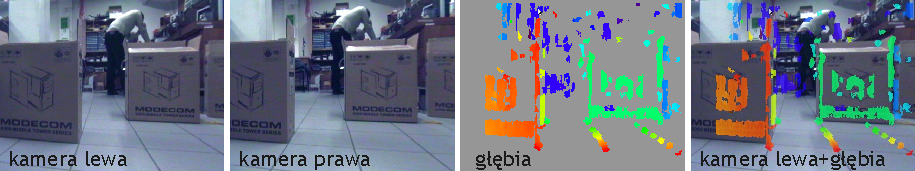
\includegraphics{../../Common/img/stereo_1}
\caption[Pierwsza scena testowa stereowizji]{Pierwsza scena testowa stereowizji.}
\label{fig:stereo_1}
\end{figure}

Scena na rysunku~\ref{fig:stereo_2} zawiera przeszkody pokryte bardziej zróżnicowaną
teksturą, dzięki czemu są one znacznie lepiej wykrywane, a mapa głębi jest bardziej
wypełniona.

Ostatni eksperyment (rysunek~\ref{fig:stereo_3}) miał na celu pokazanie problemu
przy wykrywaniu dużych, jednolitych obiektów. Tablica zajmuje dużą część obrazu
i stanowi poważną przeszkodę dla robota. Na mapie głębi jednak oznaczone są jedynie
jej boczne krawędzie, co mogłoby doprowadzić do próby przejazdu pomiędzy nimi.

\begin{figure}[h!]
\centering
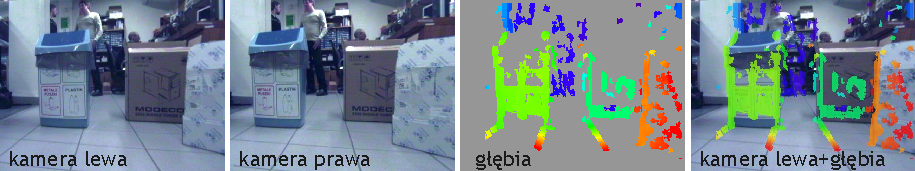
\includegraphics{../../Common/img/stereo_2}
\caption[Druga scena testowa stereowizji]{Druga scena testowa stereowizji zawierająca obiekty o zróżnicowanej teksturze.}
\label{fig:stereo_2}
\end{figure}

\begin{figure}[h!]
\centering
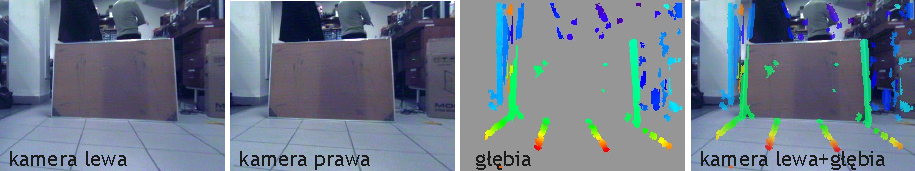
\includegraphics{../../Common/img/stereo_3}
\caption[Trzecia scena testowa stereowizji]{Trzecia scena testowa stereowizji pokazująca problemy z dużymi, jednolitymi przeszkodami.}
\label{fig:stereo_3}
\end{figure} 

%-------------------------------------------------------------------------------
\subsection{Światło strukturalne -- Microsoft Kinect}
%-------------------------------------------------------------------------------

Celem pomiarów było porównanie działania sensora Kinect i pary stereowizyjnej.
W tym celu przeanalizowano te same sceny, a obrazy wynikowe przedstawione są
poniżej. Największą różnicę widać w pokryciu obrazu na mapie głębi (w przypadku
Kinecta fragmenty nierozpoznane oznaczane są na czarno). Drugą różnicą, której
nie widać na obrazkach, jest prędkość działania. W przypadku sensora
firmy Microsoft algorytm jest zaimplementowany sprzętowo, co ma dwie zalety:
po pierwsze system komputera sterującego jest mniej obciążony, po drugie niezależnie
od jego obciążenia akwizycja danych działa z prędkością 30 klatek na sekundę.

\begin{figure}[h!]
\centering
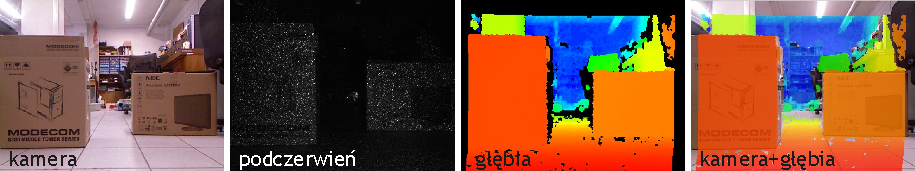
\includegraphics{../../Common/img/kinect_1}
\caption[Kinect -- pierwsza scena testowa]{Kinect -- pierwsza scena testowa}
\label{fig:kinect_1}
\end{figure}

Na rysunkach pokazany jest obraz z kamery RGB orazbraz widziany przez sensor
podczerwieni. Mapa głębi wyliczona na podstawie tego obrazu jest dodatkowo nakładana
na obraz RGB aby pokazać, w jaki sposób punkty z mapy głebi są skalibrowane z obrazem RGB.
Ogólnie dane dostarczane przez ten sensor są dużo lepszej jakości niż uzyskiwane
ze stereowizji, jednak istnieją przypadki trudne. Jednym z nich jest wykrywanie
wąskich, ciemnych przedmiotów (takich jak nogi od krzesła widoczne na
rysunku~\ref{fig:kinect_3}). Obiekty takie są zbyt małe, aby ich pokrycie przez
wzór referencyjny było odpowiednio duże, dodatkowo czarny kolor w dużym stopniu
pochłania światło podczerwone utrudniając ich lokalizację. W przypadku
korzystania ze stereowizji podobne przypadki nie stanowią problemu, ponieważ
wąskie, wyraźnie widoczne linie w obrazie są wykrywane jako punkty charakterystyczne
i są wykorzystywane w procesie tworzenia mapy dysparycji (można to zaobserwować
na rysunku~\ref{fig:stereo_3}, gdzie pomimo słabego wykrywania całej powierzchni
podłogi doskonale zaznaczane są czarne linie fug pomiędzy płytkami).

\begin{figure}[h!]
\centering
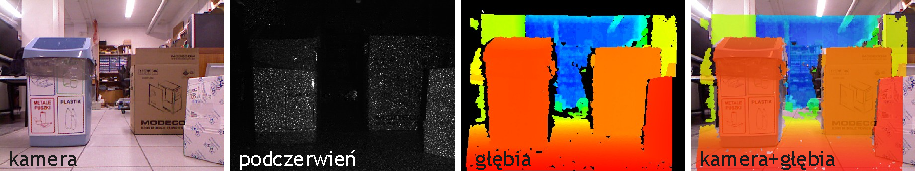
\includegraphics{../../Common/img/kinect_2}
\caption[Kinect -- druga scena testowa]{Kinect -- druga scena testowa}
\label{fig:kinect_2}
\end{figure}

\begin{figure}[h!]
\centering
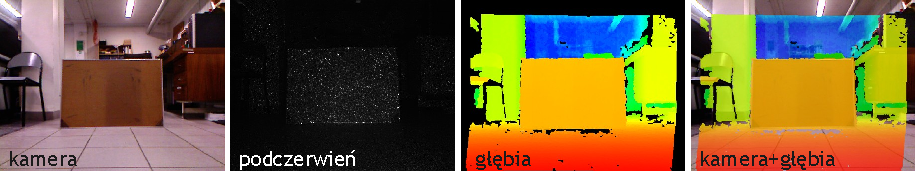
\includegraphics{../../Common/img/kinect_3}
\caption[Kinect -- trzecia scena testowa]{Kinect -- trzecia scena testowa}
\label{fig:kinect_3}
\end{figure}

\cleardoublepage
% !TeX root = main.tex


\begin{savequote}[70mm]
,,''
\qauthor{}
\end{savequote}

\chapter{Nawigacja robotów mobilnych}
\label{chap:nawigacja}

Całe zadanie nawigacji robota mobilnego może zostać podzielone na kilka głównych
składników \cite[cz.~9]{szynkiewiczWR}:

\begin{itemize}
  \item precepcję,
  \item samolokalizację robota,
  \item wnioskowanie i/lub planowanie,
  \item tworzenie mapy otoczenia,
  \item generowanie trajektorii i omijanie przeszkód.
\end{itemize}

W zależności od potrzeb, nie wszystkie z nich muszą być uwzględnione w systemie
sterowania (np. roboty mogą poruszać się w terenie, którego mapa jest nieznana
i nie jest wymagane jej tworzenie, bądź też a priori zakłada się brak
przeszkód na trasie i nie uwzględnia problemu ich wykrywania). Niniejszy
rozdział opisuje ogólne metody realizacji poszczególnych elementów systemu.

\section{Percepcja}

Ta część systemu odpowiada za gromadzenie wiedzy o stanie zarówno samego robota,
jak i otaczającego go środowiska, w którym operuje. Dokonuje się tego przez
akwizycję danych z czujników a następnie wybieranie tych informacji, które mają
znaczenie w nawigacji. 

\subsection{Klasyfikacja czujników}

Istnieje cały szereg różnych
czujników, które ogólnie można pogrupować ze względu na rodzaj mierzonych
wielkości (wyróżniamy proprioreceptory -- czujniki mierzące wartości parametrów
wewnętrznych robota,oraz eksteroreceptory -- mierzące wartości parametrów
otoczenia) oraz wpływ na otoczenie (tutaj mamy podział na czujniki bierne i
aktywne)~\cite{siegwart}.


\subsubsection{Proprioreceptory}

Proprioreceptory mierzą parametry określające w pewien sposób wewnętrzny stan
robota, takie jak prędkość silników czy napięcie akumulatorów. Wykorzystywane są
przy wyznaczaniu pozycji robota (czujniki odometryczne), sterowaniu (prędkość
obrotowa silników) czy diagnostyce jego podzespołów.

\subsubsection{Eksteroreceptory}

Eksteroreceptory pozyskują informację z otoczenia robota, takie jak natężenie
światła czy amplituda dźwięku. Można za ich pomocą mierzyć odległość,
orientację, lokalizować zewnętrzne obiekty aż wreszcie budować mapy.
Ważne jest to, że konkretne sensory są przypisywane do proprio- lub
eksteroreceptorów w zależności od ich zastosowania, a nie typu mierzonej
wartości (np. czujnik temperatury zamontowany na radiatorze silnika jest
czujnikiem wewnętrznym, a ten sam czujnik mierzący temperaturę otoczenia robota
jest już czujnikiem zewnętrznym).

\subsection{Podstawowe klasy czujników}

\section{Samolokalizacja}

Pod pojęciem samolokalizacji robota rozumie się określenie bieżącej pozycji
robota w pewnym, ustalonym układzie odniesienia. Do obliczeń wykorzystywane mogą
być dane uzyskiwane z czujników robota, 

\subsection{Klasyfikacja metod lokalizacji}

Metody lokalizacji robotów mobilnych można podzielić biorąc pod uwagę różne
kryteria. Kilka możliwych podziałów przedstawione jest w dalszej części
rozdziału, wraz z przykładami.

\subsubsection{Metody lokalne i globalne}

W zależności od lokalizacji układu odniesienia metody lokalizacji możemy
podzielić na lokalne i globalne. W metodach lokalnych układ odniesienia, w
którym następuje lokalizacja jest związany z punktem, z którego robot rozpoczyna
pracę (a więc początkowe położenie robota jest zerowe bądź wskazane przez
operatora), tak więc rozpoczynając pracę z faktycznie różnych punktów i
wykonując tę samą trajektorię (zakładając, że w ogóle może ją w każdym
przypadku wykonać), mimo takiej samej pozycji wyliczonej przez układ
lokalizacji robot będzie się znajdował w różnych miejscach.

Metody globalne operują z kolei w układach odniesienia związanych z elementami,
które nie są bezpośrednio zależne od robota. Mogą to być układy związane z danym
pomieszczeniem (z ustalonym odgórnie punktem zerowym) bądź takie jak układ
współrzędnych geograficznych, jak również oparte o mapę i lokalizujące robota
względem umieszczonych na niej obiektów. W takich metodach kluczowe jest
określenie pozycji początkowej, które nie zawsze jest łatwe do wykonania.
Korzystając z odbiorników GPS łatwo zlokalizować robota w przestrzeni otwartej,
trudniej jest to wykonać w pomieszczeniach. Rozwiązują to metody czynne, których
opis znajduje się w dalszej części rozdziału.

\subsubsection{Środowisko statyczne i  dynamiczne}

Poprzez określenie środowiska statycznego rozumie się takie otoczenie, w którym
ruch innych obiektów oprócz robota nie występuje bądź jest niewykrywalny przez
jego czujniki. Podczas pracy w środowisku dynamicznym (a więc takim, gdzie
pomimo braku ruchu robota czujniki rejestrują ruch przeszkód) algorytmy
lokalizacji muszą uwzględniać ten fakt i stosować różne rodzaje filtrowania
danych tak, aby ruch przeszkód wokół robota nie powodował zmian jego wyliczonego
położenia. Metodami odpornymi na zmiany w otoczeniu robota są wszystkie te,
które wykorzystują informacje o przesunięciu odczytywane z czujników
przesunięcia (np. odometryczne bądź inercyjne), wrażliwe mogą być z kolei metody
wykorzystujące odczyty laserowe.

\subsubsection{Metody bierne i czynne}

Przy biernych metodach lokalizacji do określenia pozycji robota jego ruch
(a dokładniej ruch sensorów) nie jest konieczny. Tak działa chociażby GPS, oraz
wszystkie metody wykorzystujące zewnętrzne nadajniki (np. latarnie radiowe). W
metodach czynnych do dokładnego określenia pozycji robota wymagany jest jego
ruch. W takim przypadku możliwe jest dowolne początkowe położenie w układzie
współrzędnych (bądź na mapie), a wraz z ruchem robota kolejne obserwacje
doprowadzają do zawężenia przestrzeni możliwych rozwiązań, a po pewnym czasie
doprowadzają do podania jesnego, ostatecznego położenia. Takimi metodami są np.
różnego rodzaju filtry cząsteczkowe i inne metody probabilistyczne.


\subsubsection{Metody względne i bezwzględne}


\section{Tworzenie mapy}

\subsection{Rodzaje map}

\section{Generowanie trajektorii}


\cleardoublepage
% !TeX root = main.tex


\begin{savequote}[70mm]
,,Z maszyną nie ma dyskusji. Jeśli chce się z~niej korzystać, musi się jej słuchać.''
\qauthor{Antoni Kępiński -- Rytm życia}
\end{savequote}


\chapter{Baza sprzętowa}
\label{chap:sprzet}

%%%%%%%%%%%%%%%%%%%%%%%%%%%%%%%%%%%%%%%%%%%%%%%%%%%%%%%%%%%%%%%%%%%%%%%%%%%%%%%%
%%%%%%%%%%%%%%%%%%%%%%%%%%%%%%%%%%%%%%%%%%%%%%%%%%%%%%%%%%%%%%%%%%%%%%%%%%%%%%%%

\section{Robot mobilny Elektron}

Robot mobilny Elektron powstał w roku 2007 jako efekt współpracy Instytutu Automatyki
i Robotyki oraz Instytutu Automatyki i Informatyki Stosowanej Politechniki Warszawskiej
\cite{SzynkiewiczEtal06}. Został zaprojektowany jako platforma laboratoryjna,
przeznaczona do badań nad systemami sterowania i nawigacji robotów mobilnych,
czemu sprzyjać miała modułowa konstrukcja zarówno części mechanicznej, jak i systemu
sterowania. Od momentu powstania robot poddawany był kolejnym modernizacjom,
mającym na ceu zarówno dołączenie nowych zestawów czujników, jak i umożliwienie
sterowania robota przy wykorzystaniu nowych struktur programowych. Pierwotnie Elektron
sterowany był przy wykorzystaniu środowiska Player/Stage, w ramach niniejszej pracy
robot został uruchomiony wykorzystując system ROS (więcej na ten temat w
rozdziale~\ref{chap:programowanie}).


\begin{figure}[h!]
\centering
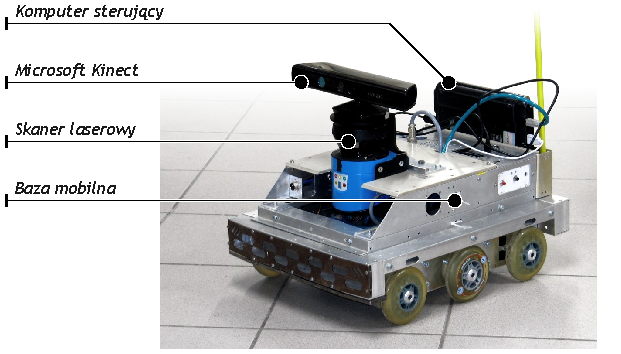
\includegraphics{../../Common/img/elektron/elektron_desc}
\caption[Robot mobilny Elektron]{Robot mobilny Elektron ze wstępnie zamocowanym
sensorem Kinect.}
\label{fig:elektron}
\end{figure}

%-------------------------------------------------------------------------------
\subsection{Konstrukcja mechaniczna}
%-------------------------------------------------------------------------------

Baza jezdna robota jest sześciokołową platformą o napędzie różnicowym na wszystkie
koła. Robot ma budowę modułową i w jej skład wchodzą moduły: napędowy (monolityczny
blok zawierający silnik, przekładnię, trzy połączone koła oraz enkoder mierzący
ich położenie), rama centralna umożliwiająca szybki montaż dodatkowych modułów oraz
dwa niezbędne moduły elektroniczne - sekcja zasilania oraz sterowania. Bazowe podwozie
wykonane jest w całości z profili aluminiowych, ma wymiary 500x380x220mm i całkowicie
osłania wszystkie wewnętrzne systemy robota.

\begin{table}[h!]
\caption{Parametry robota Elektron}
\centering
\small
\begin{tabular*}{0.6\textwidth}{@{\extracolsep{\fill}} lr}
\toprule
\textbf{Właściwości kinematyczne}\\
\midrule
Maksymalna prędkość liniowa & 0.25m/s \\
Maksymalna prędkość kątowa & 85\textdegree/s\\
\midrule
\textbf{Zasilanie} \\
\midrule
Pojemność akumulatorów & 2x7200mAh \\
Napięcie akumulatorów & 2x12V \\
Dostępne napięcia zasilania & 5V, 12V, 24V \\
Dodatkowe & zintegrowana ładowarka \\
\bottomrule
\end{tabular*}
\label{tab:gyro_params}
\end{table}

Pierwotnie komputer sterujący robotem był umieszczony wewnątrz ramy (był to komputer
przemysłowy z procesorem klasy Pentium III), obecnie do sterowania wykorzystywany
jest netbook EeePC mocowany w kieszeni z tyłu.

%-------------------------------------------------------------------------------
\subsection{Moduły sensoryczne}
%-------------------------------------------------------------------------------

Robot Elektron wyposażony jest w kilka niezależnych zestawów czujników. Przy realizacji
zadania wykorzystane zostały: układ pomiaru odometrycznego, układ zawierający żyroskop,
układ kamery trójwymiarowej w postaci urządzenia Microsoft Kienct oraz skaner laserowy
Sick LMS100. Układ pomiaru odometrycznego składa się z dwóch enkoderów optycznych
umieszczonych w module napędowym. Każdy z nich jest w stanie zmierzyć kt obrotu kół
napędowych z rozdzielczością 4000 impulsów na obrót. W projekcie zrezygnowano montowania
dodatkowych czujników na wałach silników.

Drugi z wymienionych układów służy do pomiaru prędkości kątowej w celu wspagania
obliczeń położenia i orientacji robota. Zawiera żyroskop Analog Devices ADXRS401,
połaczony z mikrokomputerem jednoukładowym PIC16F688, przy pomocy którego pomiary
przekazywane są do komputera sterującego za pomocą interfejsu USB.

% TODO: Sprawdzić model mikrokontrolera na płytce z żyroskopem

\begin{table}[h!]
\caption{Parametry żyroskopu ADXRS401}
\centering
\small
\begin{tabular*}{0.6\textwidth}{@{\extracolsep{\fill}} lr}
\toprule
\textbf{Czułość}\\
\midrule
Zakres pracy & \textpm 75\textdegree/s \\
Współczynnik skali & 12.75 - 17.25 mV/\textdegree/s \\
\midrule
\textbf{Temperatura pracy} \\
\midrule
Zakres temperatur & -40 - +85\textdegree C \\
Współczynnik temperaturowy & 8.5mV/K \\
\bottomrule
\end{tabular*}
\label{tab:gyro_params}
\end{table}


%%%%%%%%%%%%%%%%%%%%%%%%%%%%%%%%%%%%%%%%%%%%%%%%%%%%%%%%%%%%%%%%%%%%%%%%%%%%%%%%
%%%%%%%%%%%%%%%%%%%%%%%%%%%%%%%%%%%%%%%%%%%%%%%%%%%%%%%%%%%%%%%%%%%%%%%%%%%%%%%%

\section{Microsoft Kinect}

Jest to kontroler do gier dla konsoli Xbox wykorzystujący analizę światła
strukturalnego. Pomimo jego pierwotnego przeznaczenia, kilka dni po premierze
został opublikowany nieoficjalny sterownik umożliwiający wykorzystanie
informacji z jego czujników na komputerze PC~\cite{Giles201022}. Jego niska cena
(500PLN), dostępność wielu algorytmów ułatwiających wykorzystanie dostarczanych
przez niego informacji oraz szybkość i dokładność działania sprawiły, że został
on wybrany jako główne źródło informacji o scenie do wykorzystania w projekcie.

\begin{figure}[h!]
\centering
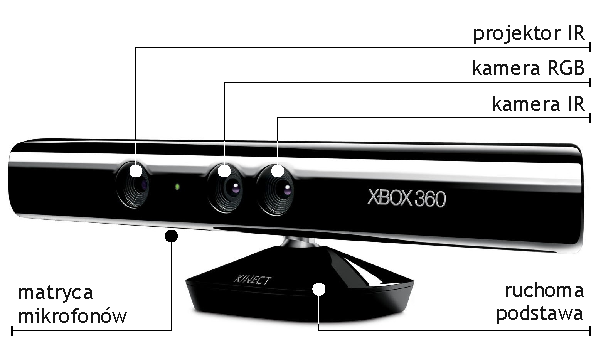
\includegraphics{../img/kinect_hardware}
\caption[Sensor Kinect firmy Microsoft]{Sensor Kinect firmy Microsoft z zaznaczonymi
kluczowymi elementami.}
\label{fig:kinect_hardware}
\end{figure}

%-------------------------------------------------------------------------------
\subsection{Budowa}
%-------------------------------------------------------------------------------

Kluczowe elementy sensora Kinect zaznaczone są na rysunku~\ref{fig:kinect_hardware}.
Pomiar głębi realizowany jest przy użyciu pary złożonej z projektora podczerwieni
oraz kamery rejestrującej obraz w tym paśmie. Kamera RGB umieszczona pomiędzy nimi
służy do rejestracji widocznej sceny, a dzięki jej kalibracji z pomiarem głębi
możliwe jest tworzenie trójwymiarowych map otoczenia z nałożoną teksturą (dane
kalibracyjne dostarczone przez producenta są zapisane bezpośrednio w urządzeniu).

\begin{figure}[h!]
\centering
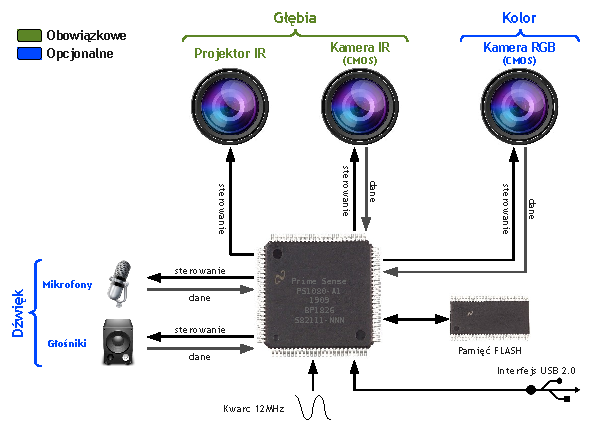
\includegraphics{../../Common/img/primesense}
\caption{Schemat blokowy sensora Kinect}
\label{fig:kinect_block}
\end{figure}

Dodatkowo Kinect wyposażony jest w matrycę czterech mikrofonów, które mogą być
wykorzystane do lokalizacji źródeł dźwięku w przestrzeni, a~także podstawę umożliwiającą
pochylanie sensora w~zakresie~27\textdegree~w~górę i~w~dół.

Istotne parametry techniczne zebrane są w tabeli~\ref{tab:kinect_params}.

\begin{table}[h!]
\caption{Kinect -- parametry techniczne}
\centering
\small
\begin{tabular*}{0.6\textwidth}{@{\extracolsep{\fill}} lr}
\toprule
\textbf{Pole widzenia}\\
\midrule
Poziome & 57\textdegree \\
Pionowe & 43\textdegree \\
Zakres ruchu góra/dół & $\pm$27\textdegree \\
Efektywny pomiar odległości & 1.2m - 3.5m \\
\midrule
\textbf{Kamera RGB} \\
\midrule
Rozdzielczość & 640x480px \\
Głębia bitowa & 8 bitów \\
Prędkość & 30kl/s \\
\midrule
\textbf{Mapa głębi} \\
\midrule
Rozdzielczość & 320x240px \\
Głębia bitowa & 16 bitów \\
Prędkość & 30kl/s \\
\bottomrule
\end{tabular*}
\label{tab:kinect_params}
\end{table}

%-------------------------------------------------------------------------------
\subsection{Działanie}
%-------------------------------------------------------------------------------

Sercem urządzenia jest dedykowany układ tworzący mapę głębi na podstawie analizy
obrazu z kamery IR. W pierwszym kroku na scenę rzutowany jest specjalny wzór
(przedstawiony na rysunku~\ref{fig:kinect_pattern}), a uzyskany obraz jest
rejestrowany przez kamerę działającą w paśmie bliskiej podczerwieni.

\begin{figure}[h!]
\centering
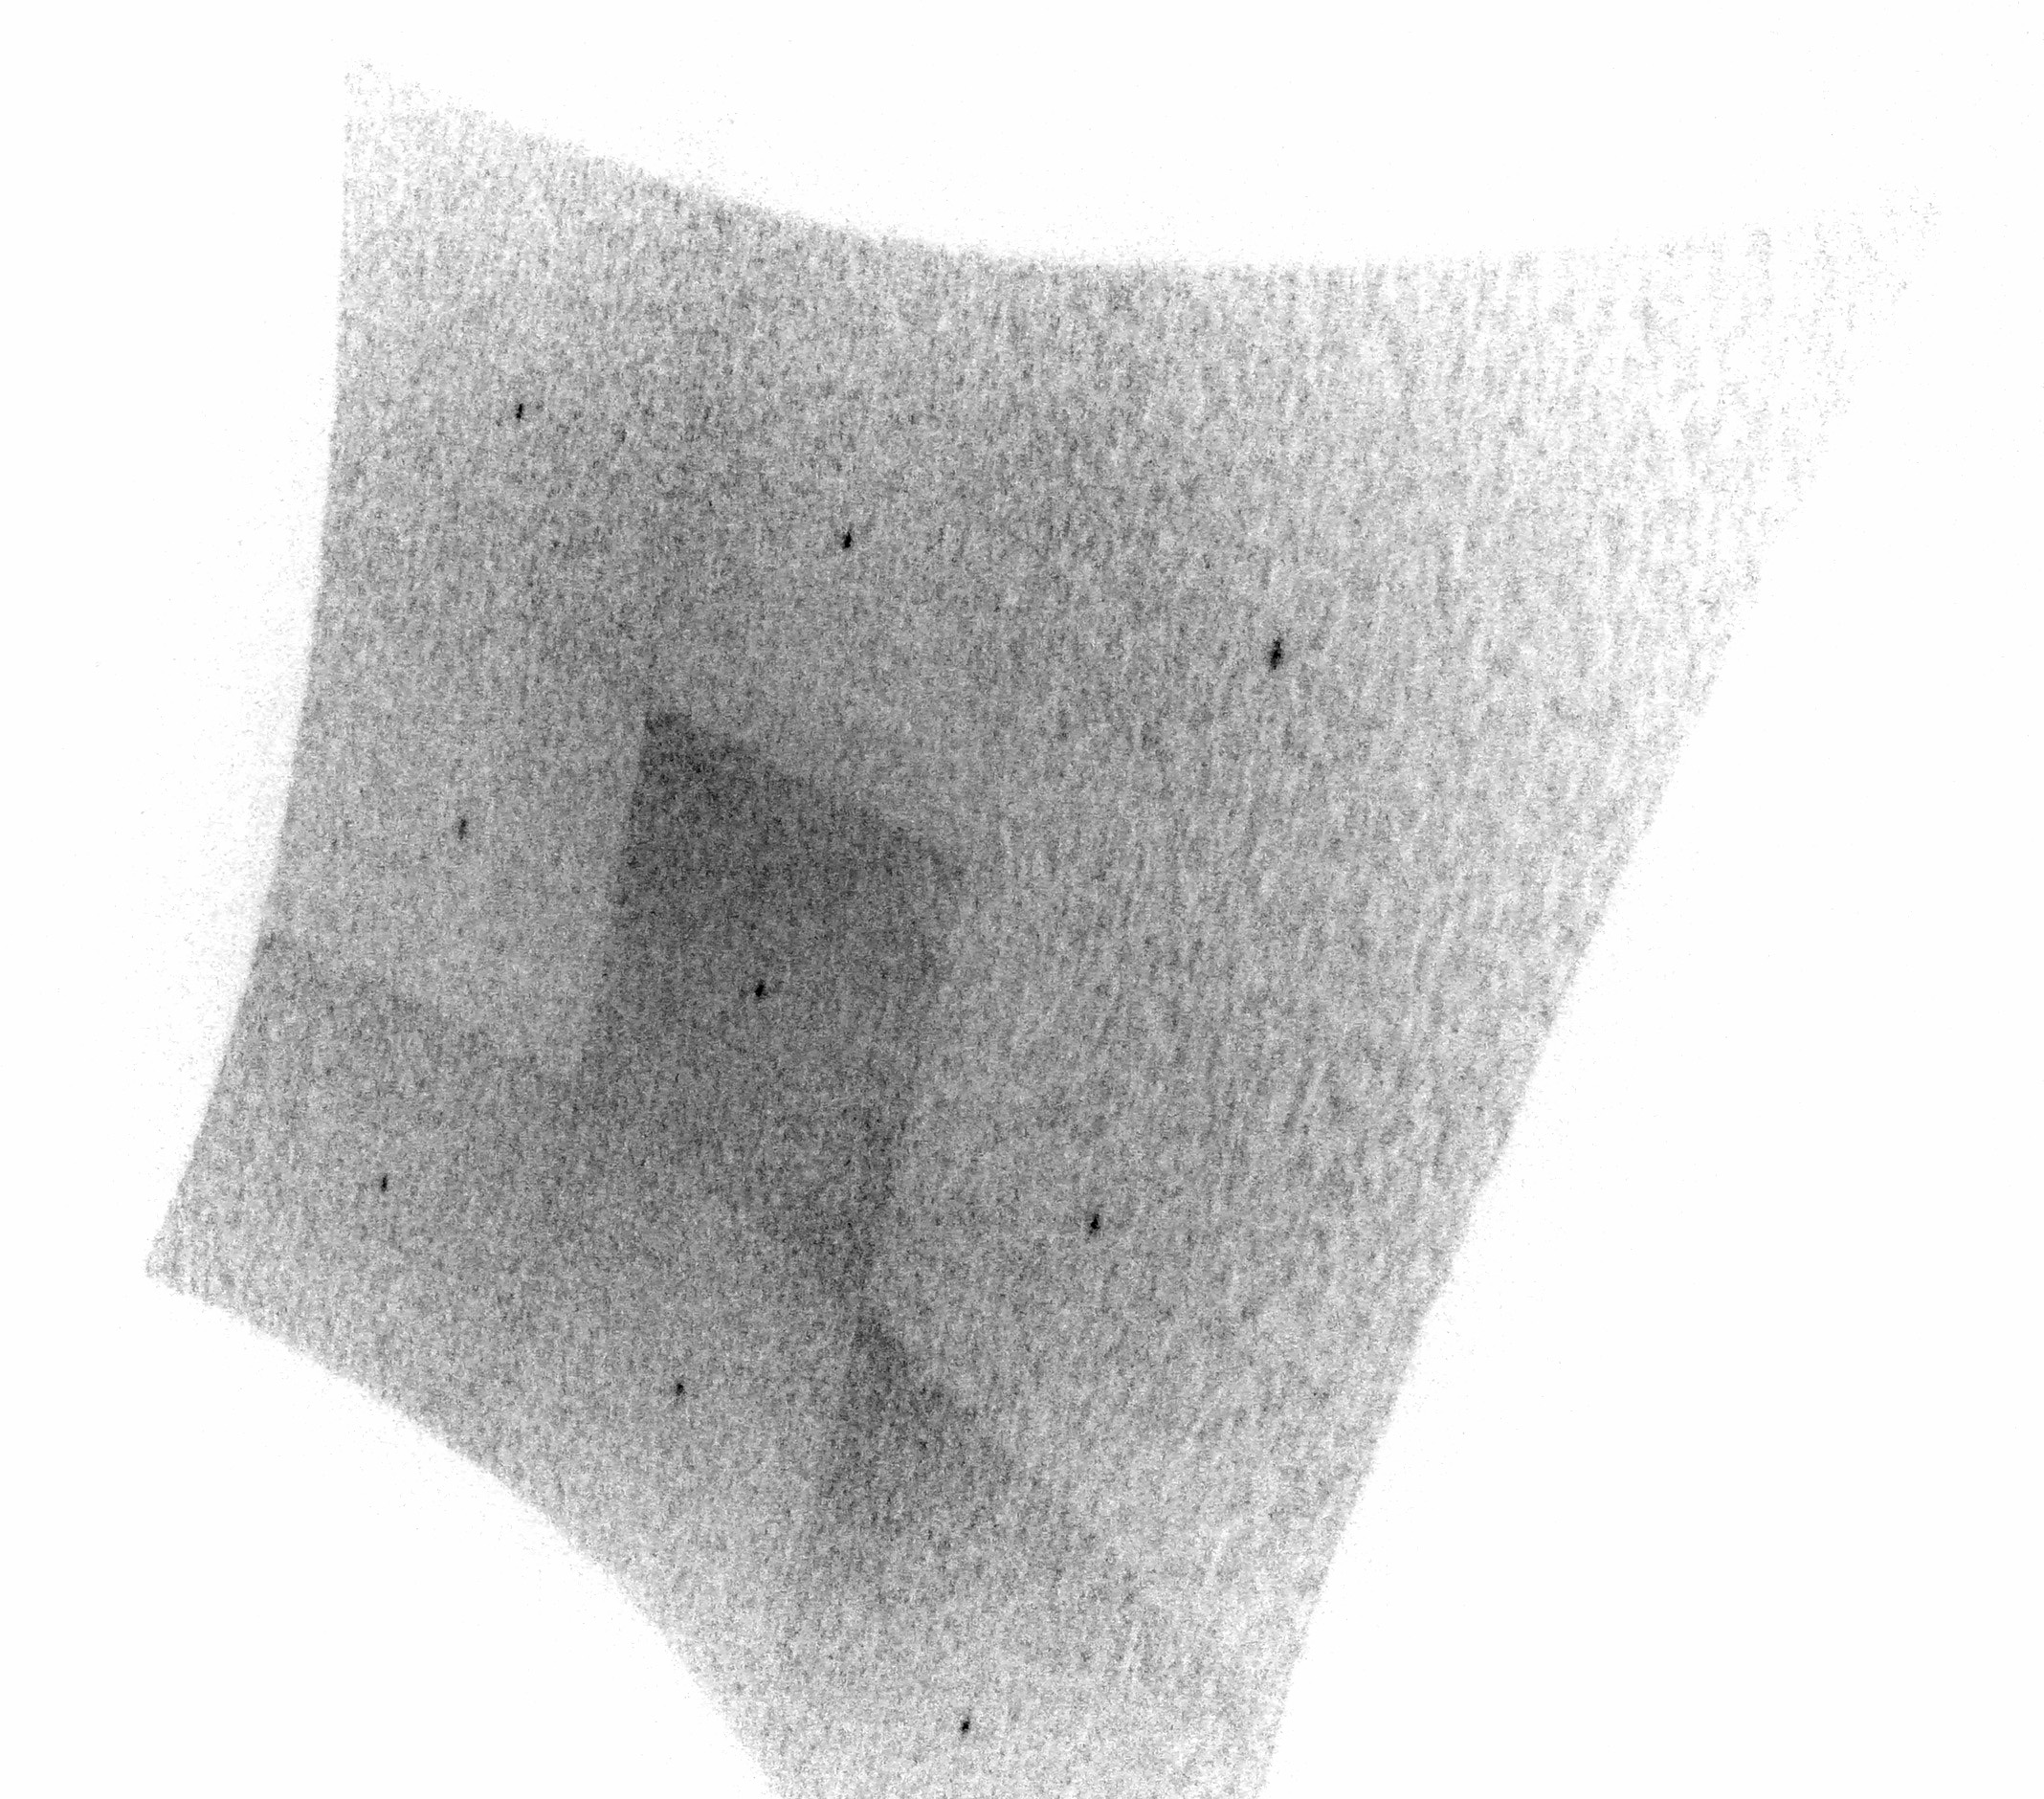
\includegraphics[width=8cm]{../img/kinect_pattern}
\caption[Wzór rzucany przez Kinect]{Wzór rzucany przez Kinect (kolory odwrócone,
ciemne punkty oznaczają miejsca oświetlane przez rzutnik podczerwieni). Źródło:
http://goo.gl/L7sJm}
\label{fig:kinect_pattern}
\end{figure}

Wzór ma specjalną strukturę, umożliwiającą poprawne zlokalizowanie analizowanych
pikseli w obrazie wzorcowym bez konieczności wielokrotnego rzutowania różnych
tekstur (tak jak przy metodzie wykorzystującej kod Graya i coraz węższe paski).
Zaczynając od największych bloków wyróżnić w nim można szachownicę 3x3 pola, a
na środku każdego z nich jaśniejszy punkt służący do lokalizacji centrum danego
segmentu. Każde z pól pokryte jest siatką punktów ułożonych w taki sposób, aby
ich bloki potwarzały się bardzo rzadko lub wcale w obrębie danego pola
szachownicy (w ten sposób wyeliminowany został problem fałszywych dopasowań
podczas porównywania z obrazem referencyjnym). Po zlokalizowaniu pozycji
pikseli w mapie wzorcowej z triangulacji wyliczane jest ich względne
przesunięcie, a z niego ostateczna mapa głębi.

%-------------------------------------------------------------------------------
\subsection{Mocowanie na robocie}
%-------------------------------------------------------------------------------

Mocując sensor na robocie należało uwzględnić ograniczoną minimalną odległość,
z jakiej Kinect wykrywa obiekty. Początkowo urządzenie zostało zamocowane na
dole robota, przed skanerem laserowym. Rozwiązanie to miało jednak dwie wady --
po pierwsze obiekty znajdujące się bliżej niż 60cm od robota nie były
wykrywane, po drugie oś optyczna sensora była pod tak ostrym kątem do podłogi,
że nie była ona praktycznie wykrywana. Na rysunku~\ref{fig:elektron} pokazana
jest druga próba mocowania, na głowicy lasera, ale okazało się, że i taka
wysokość nie jest wystarczająca, aby w pełni wykrywać obiekty przed robotem.
Ostatecznie sensor zamocowany jest bliżej tylnej części robota, kilka
centymetrów powyżej skanera Sick, i jest pochylony o 20\textdegree w dół. Taka
konfiguracja umożliwia wykrywanie przeszkód w całym pasie przed robotem,
znajdujących się nie bliżej niż 10cm od jego przednej krawędzi.
Rysunek~\ref{fig:range} przedstawia ostateczne umiejscowienie czujników
na robocie, wraz z zaznaczonymi polami widzenia Kinecta (kolor niebieski) i
skanera laserowego(kolor czerwony).

% TODO: Stworzyć schemat elektrona z zamocowanym kinectem i pokazanym polem
% widzenia kinecta i sicka


\begin{figure}[htp!]
\centering
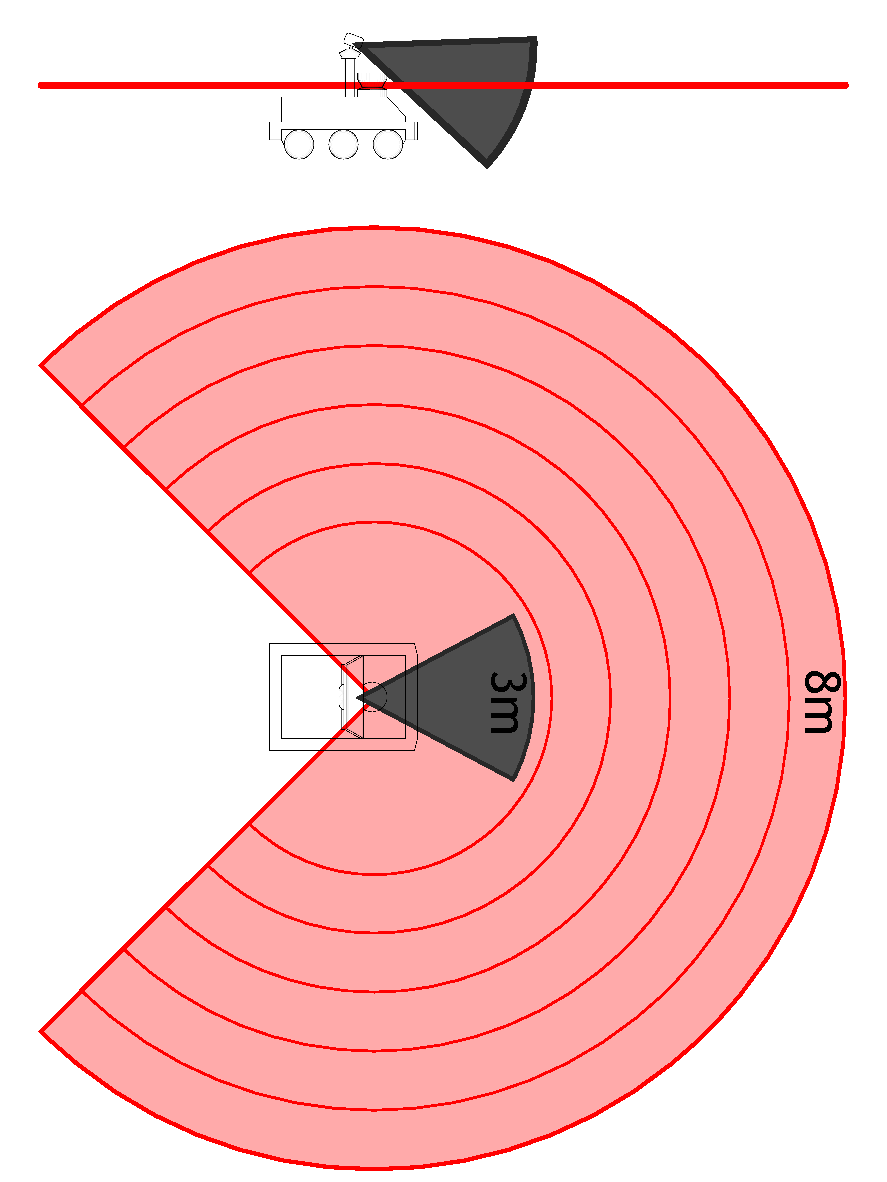
\includegraphics{../../Common/img/elektron/range}
\caption[Przybliżone zasięgi działania czujników umieszczonych na robocie
ELektron]{Przybliżone zasięgi działania czujników umieszczonych na robocie
ELektron. Kolorem czerwonym oznaczono efektywne pole działania skanera Sick,
kolorem niebieskim zasięg sensora Kinect. Dla czytelności rysunek samego robota
jest w skali większej niż pokazane zasięgi.}
\label{fig:range}
\end{figure}


%%%%%%%%%%%%%%%%%%%%%%%%%%%%%%%%%%%%%%%%%%%%%%%%%%%%%%%%%%%%%%%%%%%%%%%%%%%%%%%%
%%%%%%%%%%%%%%%%%%%%%%%%%%%%%%%%%%%%%%%%%%%%%%%%%%%%%%%%%%%%%%%%%%%%%%%%%%%%%%%%

\section{Skaner laserowy SICK LMS100}

Skaner laserowy firmy Sick, model LMS100 jest urządzeniem zdolnym do mierzenia
odległości do otaczających obiektów w zakresie 270\textdegree. Pomiar dokonywany
jest przy użyciu promienia lasera, który odbijany jest od obracającego się
lustra. Po odbiciu od przeszkody dokonywany jest pomiar czasu, po jakim wiązka
wróciła do detektora, a z tego wyliczana jest odległość. W przypadku modelu
LMS100 dla każdego promienia dokonywane są faktycznie dwa pomiary, dzięki czemu
dużo rzadziej zdarzają się zafałszowane wyniki (spowodowane np. odbiciem
promienia od kropli deszczu), dodatkowo wraz z odległością każdy pomiar ma
dołączoną intensywność wracającego światła (to z kolei pozwala np. wykrywać
szyby znajdujące się przed robotem -- powodują one powrót pierwszego impulsu o
niskim natężeniu).

\begin{figure}[h!]
\centering
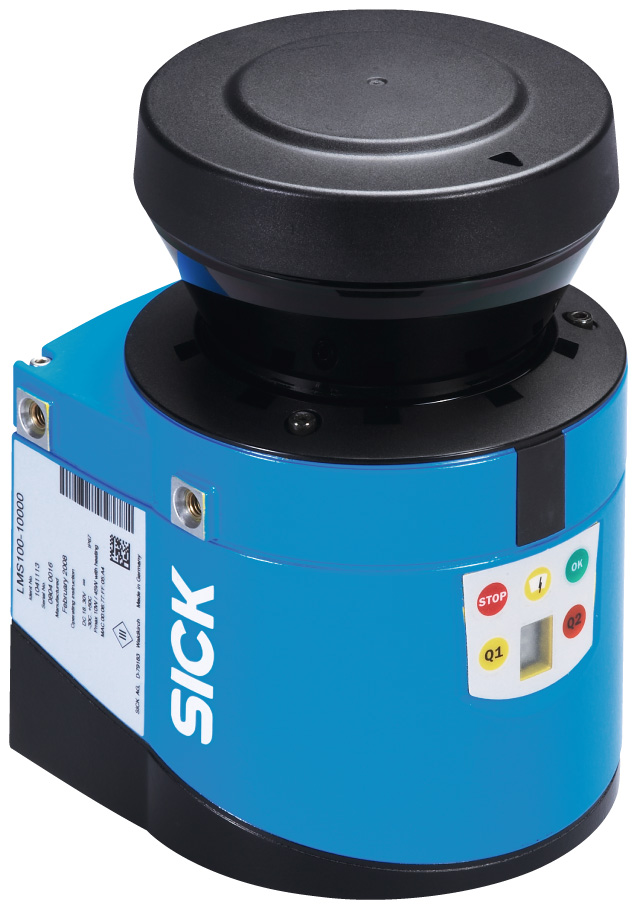
\includegraphics[height=5cm]{../img/LMS100}
\caption{Skaner laserowy SICK LMS100}
\label{fig:sick}
\end{figure}

Początkowo na robocie Elektron zamontowany był skaner laserowy Sick LMS200
(pokazany na rysunku~\ref{fig:sick_obrotnica}), jednak z powodu jego wielkości
utrudnione było montowanie dodatkowych elementów na korpusie robota. Dlatego też
został on zastapiony mniejszymi skanerami LMS100, które dodatkowo mają
korzystniejsze parametry techniczne przy wykorzystaniu na robotach mobilnych
operujących w pomieszczeniach zamkniętych (ich zestawienie zebrane w
tabeli~\ref{tab:sick_params}).

\begin{table}[h!]
\caption{Parametry skanera laserowego Sick LMS100}
\centering
\small
\begin{tabular*}{0.8\textwidth}{@{\extracolsep{\fill}} lcc}
\toprule
\textbf{Parametry skanu} & LMS100 & LMS200\\
\midrule
Zasięg & 20m & 20m \\
Rozdzielczość kątowa & 0.25\textdegree / 0.5\textdegree & 0.25\textdegree /
0.5\textdegree / 1\textdegree \\
Kąt skanowania & 270\textdegree / 270\textdegree & 100\textdegree /
180\textdegree / 180\textdegree \\
Częstotliwość skanowania & 25Hz / 50Hz & 18Hz / 37Hz / 75Hz \\
\midrule
\textbf{Inne} \\
\midrule
Interfejs komunikacyjny & ethernet 100Mbps & RS232/422 max. 0.5Mbps \\
Pobór mocy & 12W & 20W\\
Masa & 1.1kg & 4.5kg\\
\bottomrule
\end{tabular*}
\label{tab:sick_params}
\end{table}

\subsection{Mocowanie na robocie}

Skaner zamocowany jest w przedniej części robota, na stałe. Zrezygnowanie z
mocowania na obrotowej głowicy umożliwiło jego częściowe wsunięcie do wnętrza,
przez co obniżony został poziom pracy skanera (wykrywane są obiekty na
wysokości zbliżonej do wysokości robota). Sposób zamocowania lasera zobaczyć
można na rysunku~\ref{fig:elektron}.

%%%%%%%%%%%%%%%%%%%%%%%%%%%%%%%%%%%%%%%%%%%%%%%%%%%%%%%%%%%%%%%%%%%%%%%%%%%%%%%%
%%%%%%%%%%%%%%%%%%%%%%%%%%%%%%%%%%%%%%%%%%%%%%%%%%%%%%%%%%%%%%%%%%%%%%%%%%%%%%%%

\section{Komputer sterujący}

Pierwotnie Elektron posiadał zabudowany komputer przemysłowy klasy Pentium III 900MHz.
Był on umieszczony wewnątrz robota, przez co dostęp do niego był lekko utrudniony.
Dodatkową wadą takiego rozwiązania był brak monitora -- podczas pracy w laboratorium
możliwa była jego obsługa zdalna, jednak wychodząc z robotem poza laboratorium
konieczne było zabieranie bądź dodatkowego monitora i klawiatury, bądź laptopa
w celu jego obsługi. Aby wyeliminować te niedogodności, a także zwiększyć moc
obliczeniową, komputery przemysłowe zostały zastąpione netbookami Asus Eee PC 901.
Mocowane są one w tylnej części robota, w specjalnej kieszeni, przez co jest do
nich łatwy dostęp.

\begin{figure}[h!]
\centering
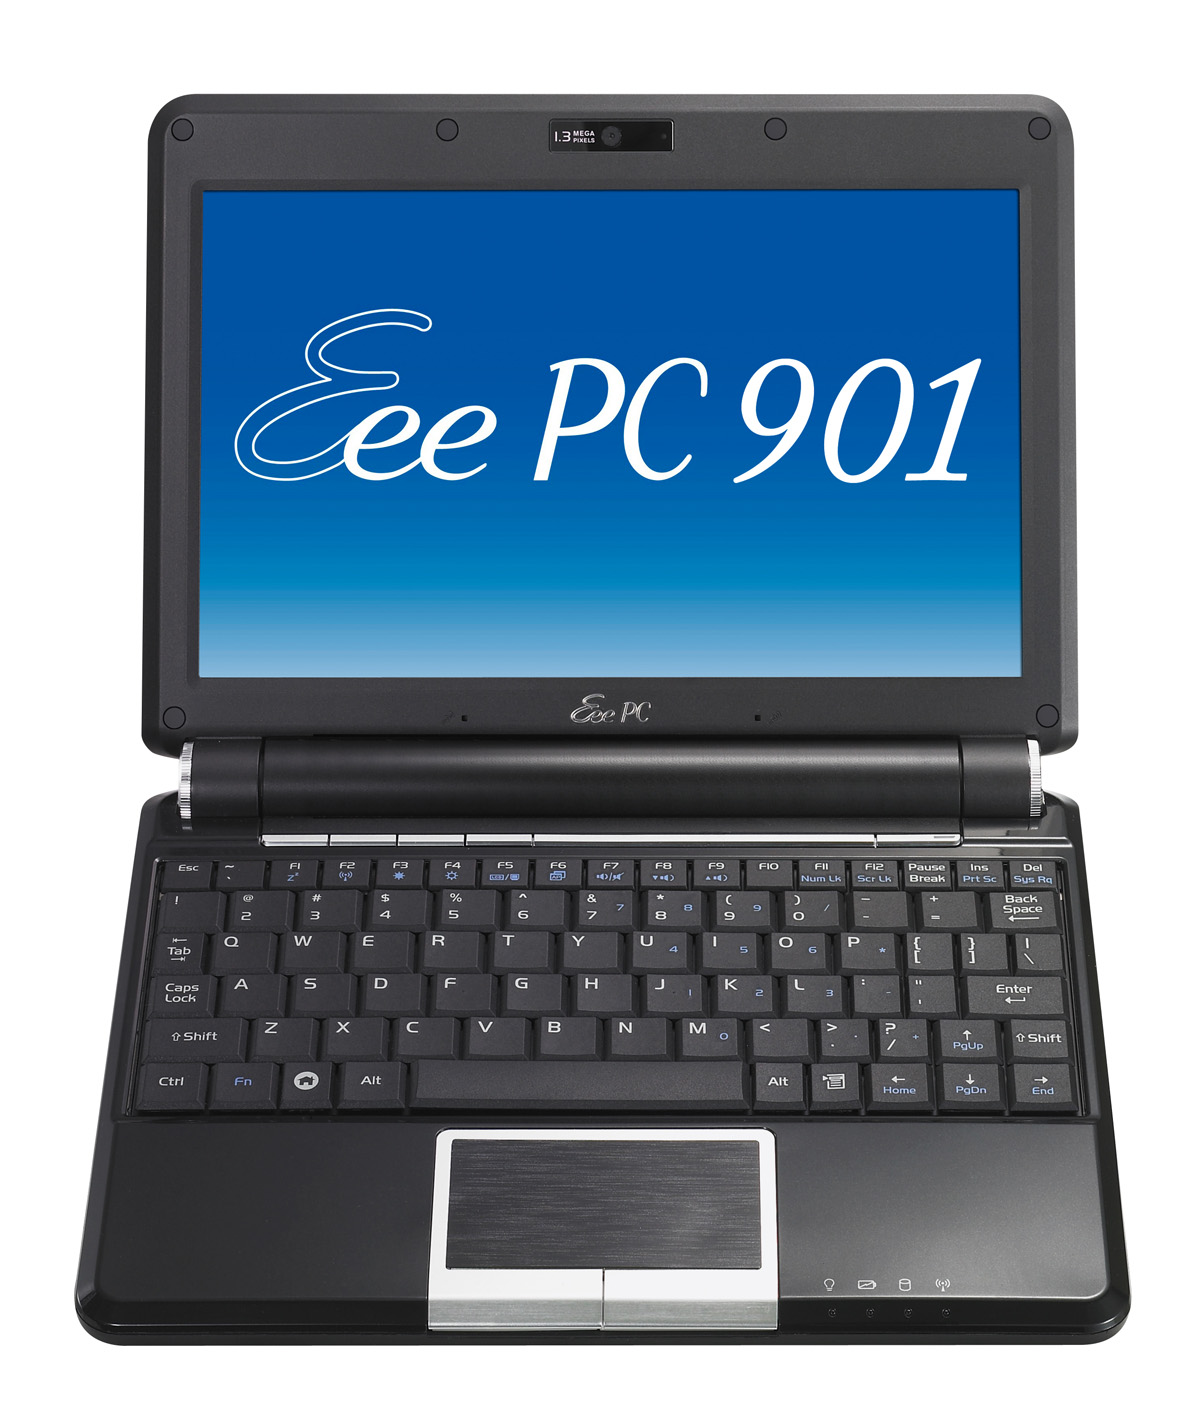
\includegraphics[height=6cm]{../img/eee}
\caption{Netbook Asus Eee PC 901}
\label{fig:eee}
\end{figure}

Konkretny model laptopa wybrany został ze względu na kilka parametrów, z których
najważniejszymi były wielkość oraz technologia wykonania dysku twardego. Wybrany
komputer posiada ekran o przekątnej 8.9", przez co cała konstrukcja jest zwarta
i niewielka, bez problemów mieszcząc się w przeznaczonym do tego miejscu (robot
z zamocowanym komputerem przedstawony jest na rysunku~\ref{fig:elektron}). W przypadku
dysku twardego kluczowe było, aby nie posiadał żadnych elementów mechanicznych,
które mogłyby doprowadzić do jego uszkodzenia podczas jazdy robota (nagłe uderzenia
czy nierówności nawierzchni). Pierwszy komputer wyposażony był w karty pamięci
CompactFlash w roli dysków twardych, wybrany model laptopa posiada natomiast
dyski twarde wykonane w technologii SSD. Najważniejsze parametry techniczne
zastosowanych komputerów zebrane są w tabeli~\ref{tab:eee_params}.
Pomimo, iż moc obliczeniowa nowych komputerów zwiększyła się w porównaniu z
rozwiązaniem pierwotnym, to i tak jest ona niewielka (jak na obecne czasy),
dlatego należy uwaznie planować wykorzystywanie czasochłonnych algorytmów i w
miarę możliwości wykorzystywać do tego inne maszyny dostępne w obrębie sieci
WiFi.

\begin{table}[h!]
\caption{Asus Eee PC 901 -- istotne parametry techniczne}
\centering
\small
\begin{tabular*}{0.6\textwidth}{@{\extracolsep{\fill}} lr}
\toprule
\textbf{Procesor}\\
\midrule
Model & Intel Atom N270\\
Taktowanie & 1.6GHz\\
Ilość rdzeni & 1 (2 wątki)\\
Architektura & 32bit \\
\midrule
\textbf{Pamięć RAM} \\
\midrule
Pojemność & 1GB \\
Taktowanie & 667MHz \\
\midrule
\textbf{Dysk twardy} \\
\midrule
Technologia & SSD \\
Pojemność & 4+8GB \\
\midrule
\textbf{Inne} \\
\midrule
Ciężar & 1.1kg \\
Pojemnośc akumulatora & 6600mAh \\
\bottomrule
\end{tabular*}
\label{tab:eee_params}
\end{table}



\cleardoublepage
% !TeX root = main.tex


\begin{savequote}[70mm]
,,''
\qauthor{}
\end{savequote}


\chapter{Programowanie robotów mobilnych}
\label{chap:programowanie}

\section{Metody programowania robotów}

Do wykorzystania wszystkich możliwości dawanych przez sprzęt zainstalowany na robocie
wymagane jest odpowiednie oprogramowanie na komputerze sterującym robota. Odpowiada
ono za zadania na wielu poziomach abstrakcji, od sterowników niskiego poziomu
komunikujących się bezpośrednio ze sprzętem, przez moduły przetwarzające dane otrzymane
bezpośrednio z sensorów do pewnej, z góry założonej postaci, aż po wysokopoziomowe
algorytmy wykorzystujące przygotowane wcześniej dane do wykonania pewnego zadania.

\section{Sterowniki wbudowane}

W przypadku prostych robotów wyposażonych w niewielką ilość czujników
i przeznaczonych do wykonywania kilku z góry okreslonych zadań stosuje się systemy
złożone z mikrokontrolera połączonego z układami sensorycznymi i sterującego pracą
całego robota. Do jego zadań należy zarówno odczyt danych z czujników, ich analiza
i przetwarzanie, a także sterowanie efektorami robota. Systemy takie mają niewielką
wydajność, ale ze względu na ich dobre dostosowanie do przewidzianego zadania działają
szybko i pozwalają na uruchomienie pętli sterowania nawet w tempie kilkuset na sekundę.
Przykładem takiego systemu może byc układ sterowania robotów sportowych. W przypadku
robotów śledzących linię ich prędkość często przekracza 2m/s, przy jednoczesnej
akwizycji i analizie danych z kilkunastu czujników i zdolności do natychmiastowej
reakcji na wykryte przeszkody.

Największą zaletą takich systemów jest ich niski koszt (często oscylujący w okolicach
kilkunastu PLN) i prostota konstrukcji (możliwość montażu na płytce uniwersalnej).
Niestety, możliwości są mocno ograniczone, a zmiana zadania wymaga często oprócz przepisania
samego algorytmu sterującego także zmian sprzętowych. Rozwiązanie tego typu nie nadaje
się do przygotowania platformy badawczej.

\section{Ramowe struktury programowe}

Drugą metodą jest podział systemu sterowania na rozłączne elementy -- samego
robota (efektor) i komunikujący się z nim komputer nadrzędny (który może być umieszczony
zarówno na robocie, jak i poza nim sterując nim zdalnie). W tym przypadku podzespoły
robota (jego układy sensoryczne, silniki itp.) mają swoje odrębne sterowniki sprzętowe
(np. układ sterownika silników może przyjmować jako sterowanie zadaną prędkość
i na jej podstawie generować odpowiednie sygnały dla silników, układy sensoryczne
mogą agregować dane z wielu czujników i wysyłać je we wstępnie przetworzonej formie
do komputera sterującego). Na komputerze sterującym uruchomione jest oprogramowanie
komunikujące się ze sterownikami sprzętowymi i udostępniające pozyskane w ten sposób
dane zewnętrznym algorytmom sterowania.

Metody takie są elastyczne, umożliwiają łatwą zmianę zadania, jakie ma wykonywac robot,
a także wymianę poszczególnych fragmentów systemu sterowania. Dodatkowo same aplikacje
działają niejako niezależnie od sprzętu na robocie, więc możliwe jest wykorzystanie
raz napisanych algorytmów na innych robotach (o ile dostarczają one wymaganych danych
pomiarowych), jak też łatwo można zastąpić rzeczywistego robota jego symulacją w celach
testowych. Problemem jest dużo wieksza komplikacja całego układu -- wymagany jest
komputer sterujący o dużej mocy (aby możliwe było wykonywanie różnych zadań i obsługa
komunikacji), osobne sterowniki sprzętowe dla podzespołów robota (nie da się sterować
wszystkimi elementami bezpośrednio) oraz niezawodnie działająca struktura programowa
abstrachująca algorytmy sterowania od warstwy fizycznej.

W ciągu ostatnich lat powstało wiele ramowych struktur programowych do sterowania
robotami, niektóre z nich specjalizowane dla jednego typu robotów (np. manipulatorów),
inne przygotowane do sterowania całą gamą różnych robotów, od platform mobilnych,
przez różnego rodzaju manipulatory, na robotach latających i pływających kończąc.
W tej części rozdziału przedstawię porównanie kilku struktur przeznaczonych do
sterowania m.in. robotami mobilnymi, wraz z zestawieniem wad i zalet każdego z rozwiązań
oraz uzasadnieniem wyboru jednego z nich.


\subsection{Player/Stage}

\cite{gerkey03playerstage}

\subsection{ROS}

\cite{288}

\cleardoublepage
% !TeX root = main.tex


\begin{savequote}[70mm]
,,Jeżeli zabałaganione biurko jest znakiem zabałaganionego umysłu, znakiem czego
jest puste biurko?''
\qauthor{Albert Einstein}
\end{savequote}


\chapter{Opis systemu sterowania}
\label{chap:software}

\section{Dekompozycja zadania}

Całe zadanie sterowania robota zostało rozdzielone na moduły odpowiedzialne
za poszczególne fragmenty systemu -- lokalizację robota (lokalną i globalną), 
wykrywanie przeszkód (przez oba dostępne sensory -- skaner laserowy i Kinect),
sterowanie samym robotem (poruszanie bazy jezdnej) oraz diagnostykę.

\begin{figure}[ht!]
\centering
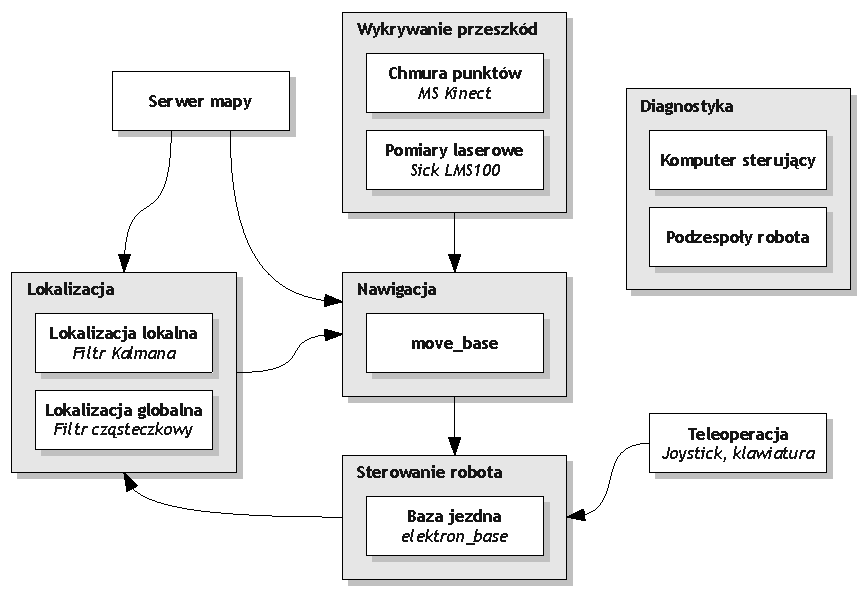
\includegraphics{../img/decomposition}
\caption{Dekompozycja systemu sterowania robota}
\label{fig:decomposition}
\end{figure}

Rysunek~\ref{fig:decomposition} przedstawia najważniejsze moduły systemu,
wraz z ogólnymi zależnościami pomiędzy nimi. Najważniejsze podsystemy
są opisane w dalszej części pracy. 

Taki podział systemu pozwala na zmniejszenie zależności pomiędzy jego elementami
do niezbędnego minimum. Poszczególne moduły komunikują się ze sobą przy pomocy 
ogólnie określonych interfejsów, a format konkretnych komunikatów nie jest 
zależny od modelu sprzętu, który jest używany do ich wygenerowania. Dzięki temu
zmiana dowolnego elementu nie wymaga wprowadzania zmian w pozostałych,
podobnie dodawanie nowych modułów (np. sensorycznych). Jest to podstawowe
wymaganie przy tworzeniu platform badawczych, na których można testować różne
algorytmy, m.in. sterowania ruchem robota, lokalizacji czy przetwarzania danych
w celu wykrywania przeszkód. 


\section{Obliczanie położenia robota}

Kluczowym zadaniem podczas pracy robota mobilnego jest określenie jego
aktualnego położenia, w układzie współrzędnych bądź to bezwzględnym (o początku
w pewnym ustalonym punkcie, np. położenie w budynku czy globalna pozycja
geograficzna) bądź pozycji względem punktu, z którego robot wystartował.
Możliwości pozycjonowania bezwzględnego wewnątrz budynków są ograniczone w
stosunku do przestrzeni otwartych. W budynkach nie sprawdza się GPS, utrudnione
jest nawigowanie względem nadajników GSM (dodatkowo jego dokładność jest dużo
za mała). Lokalizacja na podstawie naturalnych cech otoczenia w budynkach o
charakterze biurowym często może być błędna ze względu na istnienie wielu miejsc
o cechcach podobnych bądź wyglądających wręcz identycznie (np. korytarze na
różnych piętrach). Istnieją metody lokalizacji na podstawie sztucznie
umieszczonych znaczników, jednak zgodnie z założeniami zadania robot ma poruszać
się w środowku, które nie jest specjalnie przygotowane (a więc metody oparte o
pozycjonowanie względem latarni podczerwonych czy innych znaczników odpadają).
Z tego względu globalna pozycja robota nie jest wyznaczana, a podczas
autonomicznego dojazdu do celu rolą użytkownika jest wskazanie na mapie
przybliżonego punktu, z którego robot startuje.

W przypadku jeżdżących robotów mobilnych operujących w przestrzeniach
zamkniętych najczęściej wystarcza określenie dwuwymiarowego położenia i
orientacji robota, określonego trójką liczb $(x, y, \theta)$. W przypadku
robota Elektron dostępne są trzy niezależne źródła informacji o jego położeniu
względnym (dwa zwracające pełną trójkę, jedno określające jedynie bieżącą
orientację). Dokonując fuzji informacji uzyskiwanych ze wszystkich źródeł można
radykalnie zwiększyć jej dokładność. Rysunek~\ref{fig:diag_pos} przedstawia
przepływ danych pomiędzy modułami odpowiedzialnymi za kolejne etapy lokalizacji
robota, a każdy z nich jest opisany dokładniej w dalszej części rozdziału.

\begin{figure}[h!]
\centering
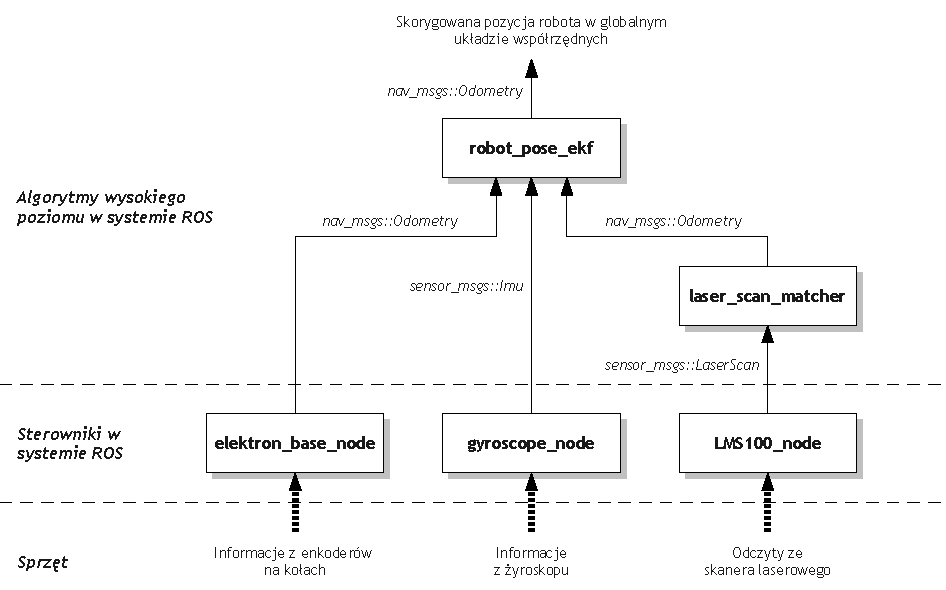
\includegraphics{../img/diag_position}
\caption{Hierarchia zadań obliczania bieżącej pozycji robota}
\label{fig:diag_pos}
\end{figure}

\subsection{Odometria}

Pierwszym źródłem informacji o położeniu robota jest moduł napędowy robota.
Wyposażony jest on w enkodery mierzące aktualną pozycję kół, dzięki czemu na
bieżąco obliczać można dystans, jaki pokonał robot. Istnieją proste wzory, które
przy znajomości chwilowej zmiany położenia kół lewej i prawej strony robota
pozwalają określić zmianę położenia i orientacji robota. Sterownik silników
robota Elektron zwraca właśnie taką informację (dokładniej ilość impulsów
enkodera zliczoną dla każdego z kół za jeden okres regulacji), oznaczmy ją przez
$(\Delta N_L, \Delta N_R)$.

\subsubsection{Obliczenie przyrostu pozycji}

Załóżmy, że w okresie $I$ sterownik silników zliczył i zwrócił do systemu
sterowania liczbę impulsów dla lewego i prawego koła $(\Delta N_L, \Delta N_R)$.
Znając dodatwe parametry:

% TODO: ładniejsze wyrównanie spisu symboli

\begin{mydescription}{5pt}
\item[$N$] liczba impulsów enkodera na pełny obrót koła,
\item[$d$] średnica koła,
\item[$b$] odstęp pomiędzy kołami robota, 
\end{mydescription}

można obliczyć dystans, jaki przebyły koła po każdej ze stron robota:

\[
\Delta S_{L,R} = \frac{\pi D}{N} \cdot \Delta N_{L,R}
\]

skąd łatwo można policzyć przesunięcie środka robota oraz zmianę jego
orientacji:

\begin{align*}
\Delta S_i &= \frac{\Delta S_L + \Delta S_R}{2} \\
\Delta \theta_i &= \frac{\Delta S_L - \Delta S_R}{b}
\end{align*}

Przy odpowiednio krótkim okresie próbkowania danych z enkoderów można założyć,
że droga pokonana przez robota w tym czasie jest odcinkiem prostej, co pozwala w
łatwy sposób obliczyć zmianę pozycji i orientacji robota:

\begin{align*}
\theta_i &= \theta_{i-1} + \Delta \theta_i \\
x_i &= x_{i-1} + \Delta S_i \cdot cos(\theta_i) \\ 
y_i &= y_{i-1} + \Delta S_i \cdot sin(\theta_i) 
\end{align*}


\subsubsection{Źródła błędów}

Odometria opiera się na bardzo prostych równaniach, dodatkowo polegając na
uproszczeniu zakładającym, że obrót koła przekłada się dokładnie na pokonany
przez nie dystans. Założenie to często się nie sprawdza, wymienić można
chociazby przypadek poślizgu kół. Wszystkie źródła błędów można zgrupować w
dwóch kategoriach: błędy systematyczne i niesystematyczne~\cite{whereami}.
Błędy z pierwszej grupy kumulują się w przybliżeniu jednostajnie przez cały czas
działania robota, przez co mogą zostać zniwelowane przez odpowiednie kalibracje.
Do błędów tych zalicza się:
\begin{itemize}
  \item faktyczna średnica kół inna od założonej,
  \item różna średnica kół po lewej i prawej stronie robota,
  \item faktyczny odstęp pomiędzy kołami różny od założonego,
  \item osie obrotu kół nie są współliniowe,
  \item skończona rozdzielczość enkoderów,
  \item częstotliwość próbkowania enkoderów.
\end{itemize}

Błędy niesystematyczne z kolei są w swej naturze nieprzewidywalne, a ich
zniwelowanie podczas działania robota jest praktycznie niemożliwe. Źródłami
błędów z tej kategorii są:
\begin{itemize}
  \item nierówności podłoża,
  \item najechanie na przeszkody,
  \item poślizgi wywołane:
  \begin{itemize}
    \item niską przyczepnością kół do podłoża,
    \item dużym przyspieszeniem,
    \item szybkimi skrętami,
    \item działaniem sił zewnętrznych,
    \item nie-punktowym kontaktem kół z podłożem.
  \end{itemize}
\end{itemize}

Występowanie tego typu błędów jest w dużym stopniu zależne od środowiska, w
jakim porusza się robot. W przypadku robota Elektron, jego sześciokołowa
konstrukcja sprzyja występowaniu problemów z tej grupy. Środek obrotu przesuwa
się w zależności od chwilowego kontaktu kół z podłożem, przez co w trakcie
obracania się może się zdarzyć, że robot oprócz orientacji zmienia także
położenie (co nie jest wykryte przez odometrię).

\subsubsection{Kalibracja}

Kilka z wymienionych wcześniej błędów można starać się zniwelować używając
stosunkowo prostych metod. Kalibracja dokładnej wielkości kół polega na
przejechaniu odcinka prostego o znanej długości, a następnie odczytaniu tej
wielkości z odometrii. Stosunek tych danych stanowi współczynnik skalujący
składowej liniowej. Współczynnik składowej kątowej (a więc kalibrację długości
osi) oblicza się wykonując robotem obrót o znany kąt (np. dwa pełne obroty,
czyli 720\textdegree), a następnie dzieląc tę wielkość przez wartość obrotu
odczytaną z odometrii. Procedura ta została wykonana dla robota Elektron, a jej
rezultaty pokazane są na wykresie~\ref{fig:odom_calib}.

\begin{figure}[ht!]
\centering
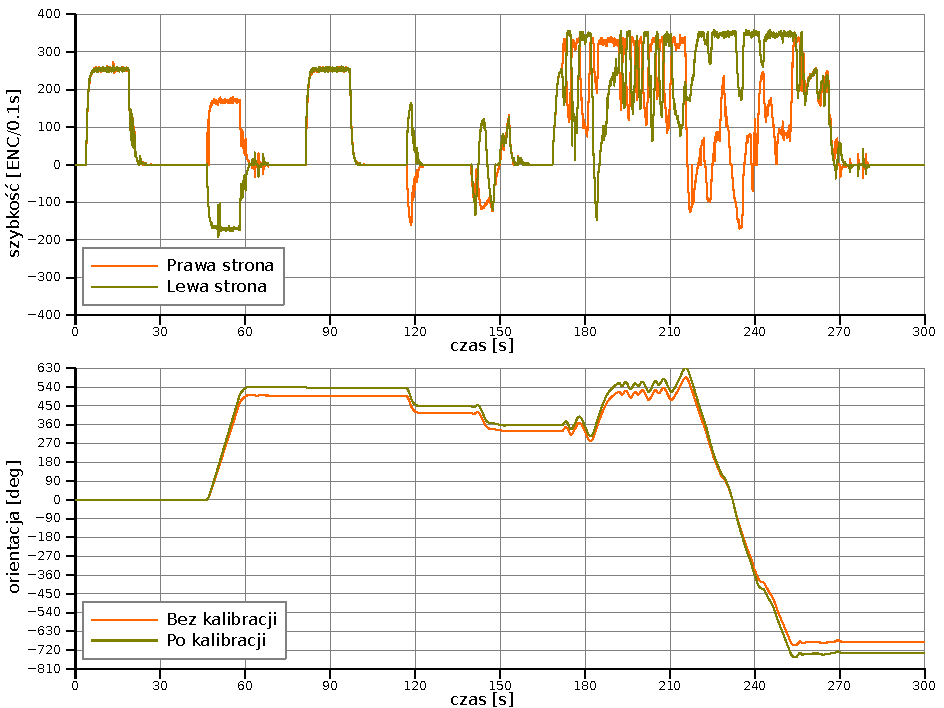
\includegraphics[width=\textwidth]{../../Common/pomiary/odom_calib}
\caption{Kalibracja odometrii robota}
\label{fig:odom_calib}
\end{figure}

\subsection{Pomiary z żyroskopu}

Korzystając z modułu wyposażonego w żyroskop można mierzyć prędkość kątową
$\omega$ robota, a z niej można sukcesywnie wyznaczać jego orientację. Wzory w
tym przypadku również nie są złożone i sprowadzają się do przemnożenia chwilowej
wartości prędkości przez czas, jaki upłynął od ostatniego pomiaru. 

\subsubsection{Źródła błędów}

Podstawowymi źródłami błędów pojawiających się podczas pomiarów przy użyciu
żyroskopów piezoelektrycznych są:

\begin{itemize}
  \item przesunięcie poziomu zera,
  \item niedokładnie dobrany współczynnik skalowania,
  \item dryf związany z temperaturą układu,
  \item dryf wartości w czasie,
  \item wpływ przyspieszenia na podawaną wartość.
\end{itemize}

Dodatkowe błędy są wnoszone przez układ konwertera analogowo-cyfrowego
(zastosowany na robocie żyroskop zwraca pomiary w postaci napięciowej).
Wiele z wymienionych błędów można zminimalizować wykonując odpowiednią
kalibrację układu pomiarowego.

\subsubsection{Kalibracja}

Wykorzystany w projekcie żyroskop ma liniową charakterystykę zależności
wartości napięcia na wyjściu od prędkości kątowej. Można ją zapisać w postaci:

\[
\omega = a \cdot (U - b)
\]

gdzie:

\begin{mydescription}{5pt}
\item[$\omega$] prędkość kątowa żyroskopu,
\item[$U$] wartość napięcia zwracana przez żyroskop,
\item[$a$] współczynnik skalujący 
\item[$b$] składowa stała pomiaru. 
\end{mydescription}

\begin{figure}[htp!]
\centering
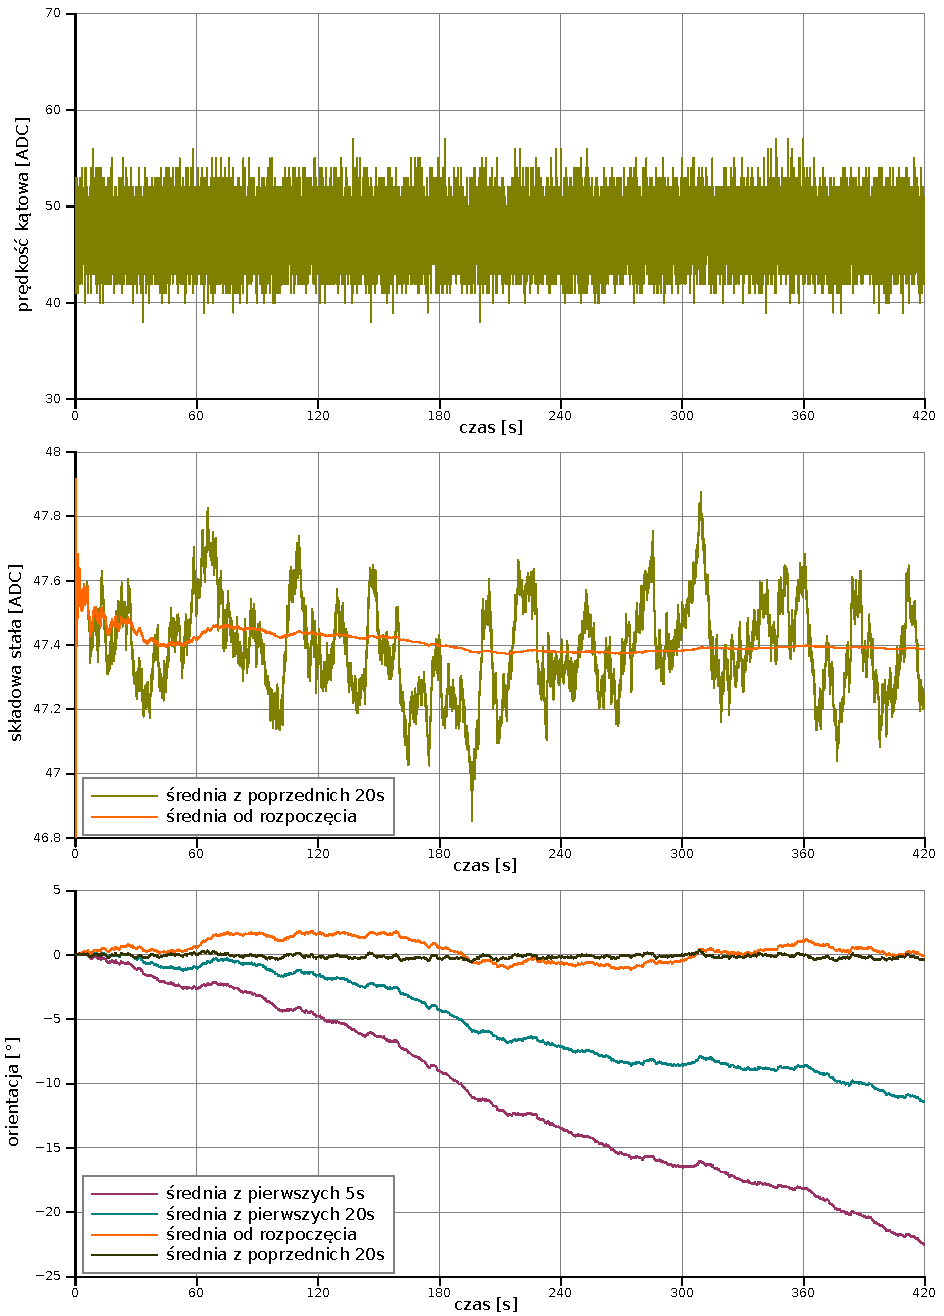
\includegraphics[width=15.5cm]{../../Common/pomiary/gyro_bias}
\caption{Kalibracja składowej stałej żyroskopu}
\label{fig:gyro_bias}
\end{figure}

Wyznaczenie składowej stałej nie jest (wbrew pozorom) zadaniem prostym. Układy
żyroskopów zrealizowane w technologii MEMS (a taki jest zastosowany)
charakteryzują się pływającą wartością składowej stałej. Prostym sposobem jej
estymacji jest uśrednienie kilkuset pierwszych pomiarów w czasie, kiedy
robot jest nieruchomy (jego prędkość kątowa jest zerowa), a następnie
traktowanie tej wartości jako składowej stałej w dalszej pracy. Niestety --
takie rozwiązanie sprawdza się jedynie na krótką metę, a w czasie pracy
orientacja robota obliczana z wykorzystaniem tego parametru zacznie coraz
bardziej oddalać się od wartości rzeczywistej. Na rysunku~\ref{fig:gyro_bias}
przedstawione są pomiary zebrane z żyroskopu przez 6 minut pracy, kiedy robot
był całkowicie nieruchomy (górny wykres, wartością oczekiwaną jest prędkość
zerowa). Środkowy wykres przedstawia średnią wartość tych pomiarów (a więc
składową stałą kumulowaną dla kolejnych pomiarów). Widać wyraźnie, że wartość ta
nie jest stabilna i podlega fluktuacjom o niekreślonej charakterystyce. Ostatni
wykres przedstawia wartość orientacji robota liczoną dla kilku długości czasu
interpolacji składowej stałej przed pomiarami (5, 20 i 120 sekund) oraz dla
składowej stałej liczonej ze wszystkich dostępnych próbek (takie rozwiązanie
nie jest możliwe do zastosowania przy pracy on-line). 

Z przedstawionego wykresu wynika, że pomiar składowej stałej jest prawidłowy dla
krótkich okresów tuż po jego wykonaniu, a wraz z upływem czasu oorientacja
robota coraz bardziej oddala się od wartości prawidłowej. Prostym sposobem na
zwalczenie tego efektu może być wykorzystanie dodatkowej informacji o braku
ruchu robota (np. z odometrii) i przeliczanie współczynnika składowej stałej
właśnie w tych momentach.

\begin{figure}[ht!]
\centering
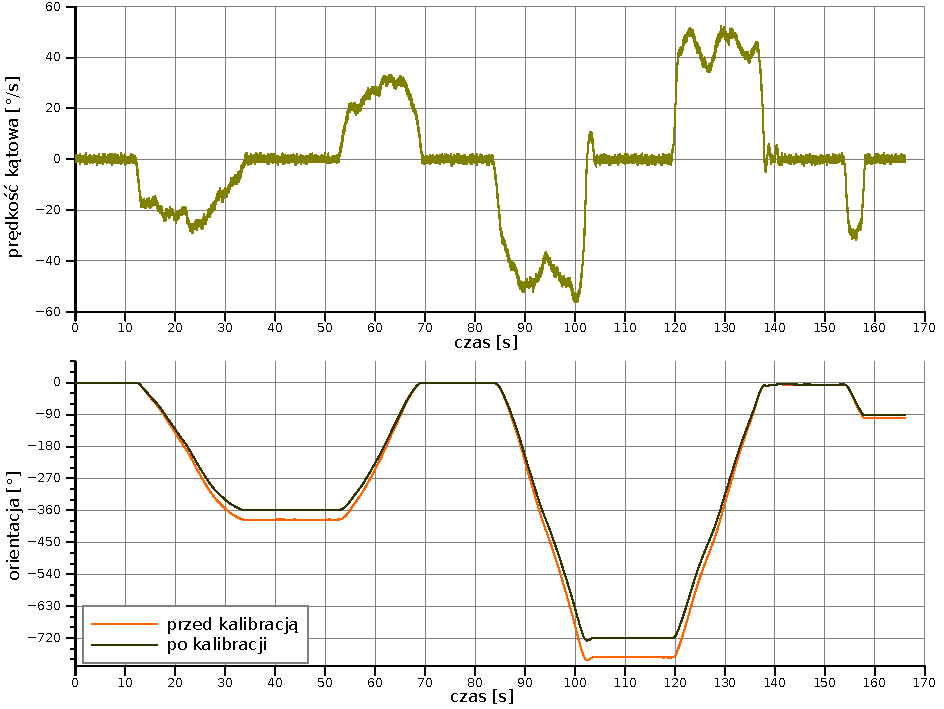
\includegraphics[width=\textwidth]{../../Common/pomiary/gyro_rot}
\caption{Kalibracja współczynnika skalowania żyroskopu}
\label{fig:gyro_rot}
\end{figure}

Drugim współczynnikiem związanym z przeliczaniem wartości napięcia zwracanego
przez żyroskop na prędkość kątową jest współczynnik skalowania. Tutaj kalibracja
jest prostsza, gdyż wartość tego parametru jest w przybliżeniu stała w czasie
dla danego układu (zależy od temperatury, ale zgodnie z założeniami robot
porusza się w obrębie pomieszczeń zamkniętych, gdzie różnice temperatur sa
niewielkie). Możliwe są dwie relatywnie proste metody kalibracji: pierwsza z
nich polega na umieszczeniu układu z żyroskopem na stoliku obrotowym i obracanie
nim ze stałą, znaną prędkością. Współczynnik skalowania wylicza się dzieląc
prędkość zadaną przez prędkość odczytaną z układu. Wadą tego rozwiązania jest po
pierwsze konieczność posiadania stolika obrotowego, po drugie problem z
ułożeniem przewodów podczas obrotów (ew. konieczność obrotu całego, ciężkiego
robota). Drugą metodą, dającą tak samo dobre rezultaty, jest obrócenie robota o
znany kąt, a następnie obliczenie szukanego parametru jako stosunku tego kąta do
skumulowanej wartości obrotu odczytanej z żyroskopu. Właśnie takie rozwiązanie
zostało zastosowane w projekcie.

Wykres~\ref{fig:gyro_rot} przedstawia odczyty z procesu kalibracji (do
policzenia współczynnika składowej stałej wybrany został okres pierwszych 10
sekund). Pierwszy wykres przedstawia wartość prędkości kątowej odczytanej z
żyroskopu (stosując domyślny współczynnik skalowania dla tego układu wynoszący
$15mV/{}^o/s$). Podczas kalibracji robot został obrócony o pełny obrót w
lewo, następnie pełny obrót w prawo, później kolejno dwa razy w lewo, dwukrotnie
w prawo, i na końcu o 90\textdegree w lewo. Oczekiwane wartości orientacji w tym
procesie wynosiły kolejno -360\textdegree, 0\textdegree, -720\textdegree,
0\textdegree, -90\textdegree. Wartości odczytane w punktach charakterystycznych
wynosiły: -385.743\textdegree, 0.047\textdegree, -774.087\textdegree,
-5.743\textdegree, -98.677\textdegree. Wartość współczynnika skalującego została
wyliczona z trzeciego odczytu:

\[
a = \frac{720^o}{774.087^o} = 0.930
\]

Orientacja robota z uwzględnionym współczynnikiem skalującym zostala
przedsationa na wspólnym wykresie razem z wartościami pierwotnymi. Widać, że
wartości obliczone są zgodne z wartościami oczekiwanymi, widoczny jest także
niekorzystny efekt związany z dryfem wartości składowej stałej (orientacja
końcowa jest poniżej zera). Parametr skalujący został następnie wprowadzony
do modułu odpowiedzialnego za obliczanie orientacji robota (orientacja liczona
w tym module jest zawijana w przedziale kąta pełnego, a więc zawiera się w
przedziale $[0, 2\pi]$, podczas kalibracji dla czytelności i uproszczenia
obliczeń dopasowanie to nie jest wykonywane).

Dodatkowo, dla uproszczenia późniejszych kalibracji zarówno odometrii jak i
żyroskopu przygotowane zostało specjalne zadanie, wykonujące automatyczną
kalibrację trzech opisanych wcześniej parametrów (współczynnik skalujący
liniowy i kątowy dla odometrii oraz współczynnik skalujący dla żyroskopu).
Opisane jest ono w rozdziale~\ref{chap:aplikacje}.

\subsection{Lokalizacja na podstawie danych ze skanera laserowego}

Ostatnim źródłem informacji, z którego można uzyskać aktualną pozycję robota
jest skaner laserowy. Informacja ta nie jest uzyskiwana wprost, jest natomiast
wynikiem działania algorytmu dopasowującego dwa kolejne skany i obliczającego
na ich podstawie względną zmianę położenia robota (a w zasadzie skanera laserowego)
pomiędzy nimi. W tym miejscu wykorzystane mogą zostać dwie implementacje
dostępne w systemie ROS: Canonical Scan Matcher~\cite{4543181} lub Polar Scan
Matcher~\cite{1545181}. Różnią się one układem współrzędnych, na którym
wewnętrznie działa algorytm (pierwszy działa w przestrzeni kartezjańskiej,
drugi korzysta z reprezentacji biegunowej). Na wyjściu oba podają estymowaną
pozycję robota względem punktu startowego.

\subsubsection{Źródła błędów}

Metoda ta, opierając się na dopasowaniu dwóch kolejnych skanów z lasera,
wrażliwa jest na zmiany w otoczeniu robota. Z samej natury algorytmów
minimalizacyjnych wynikają pewne przybliżenia (aby osiągnąć działanie w czasie
rzeczywistym warunek stopu musi określać żądaną wartość błędu w pewnym
zakresie). Nie bez znaczenia pozostają także same odczyty z lasera, na których
opierają się opisane metody -- wynikające z nich niedokładności wpływają na
osiągane wyniki, a fakt, że niektóre sceny obserowane z różnych miejsc dają
niespójne wyniki dodatkowo utrudnia ich dopasowanie.

\subsection{Rozszerzony filtr Kalmana}

Mając dostępne pomiary określające zmianę pozycji robota z wielu źródeł potrzebna jest metoda
umożliwiająca wyliczenie pewnego rodzaju ich średniej wartości, którą można już traktować
jako wypadkową zmianę pozycji. Dodatkowo każdy z pomiarów obarczony jest pewnym błedem oraz
niepewnością. W celu wyeliminowania z estymacji pozycji pomiarów, które w danej chwili
obarczone są dużym błędem oraz wyliczenia ostatecznej estymaty pozycji zastosowany został
Rozszerzony Filtr Kalmana \cite{Thrun:2005:PR:1121596}. Tradycyjny Filtr Kalmana zakłada, że procej jest procesem
liniowym, w którym zakłócenia mają rozkład Gaussowski. Cały układ obserwuje się od pewnej,
ustalonej chwili czasowej (w przypadku robota jest to np. początek ruchu), a ostateczne
rozwiązanie otrzymuje się w postaci rekurencyjnej (dzięki czemu po otrzymaniu nowych pomiarów
z czujników nie jest wymagane przeliczanie wszystkiego od początku, a jedynie uaktualnienie
stanu układu). Ze względu na nieliniowy charakter pomiarów uzyskiwanych z czujników
konieczna jest linearyzacja ich równań wokół bieżącego stanu, która jest dokonywana w
Rozszerzonym Filtrze Kalmana.

W pracy wykorzystana została implementacja opisanego filtru dostępna w systemie ROS,
umożliwiająca estymację położenia wykorzystując do trzech źródeł informacji -- dwa rodzaje
odometrii oraz pomiary z żyroskopu (czyli wszystkie źródła opisane wcześniej w tym rozdziale).
Aby umożliwić poprawne działanie tego komponentu, wszystkie pomiary muszą być opatrzone
dodatkowo ich macierzą kowariancji. W przypadku lokalizacji na podstawie odczytów z lasera
macierz kowariancji jest wypełniana przez algorytm. W przypadku żyroskopu macierz
została wypełniona stałymi wartościami, zgodnymi z zaleceniami producenta układu oraz
autorów systemu ROS. Macierz kowariancji odometrii robota zmienia się w czasie i zależy
od ruchu aktualnie wykonywanego przez robota. Jeśli robot nie wykonuje żadnego ruchu,
to niepewność zarówno odczytów prędkości liniowej jak i kątowej jest bardzo mała,
wraz ze zwiększaniem się prędkości kątowej robota niepewność jej odczytów szybko rośnie.
Dzięki temu w czasie, kiedy robot stoi nieruchomo dryf odczytów z żyroskopu oraz z lasera
nie powoduje zmiany wyliczonej orientacji robota, za to podczas faktycznego ruchu robota
czujniki te służą jako główne źródło informacji o jego obrocie.

Tutaj jeszcze wykresik z kalmanem i bez oraz jego krótka interpretacja.

odometria+żyro+laser.

\section{Monitorowanie stanu robota}

W celu monitorowania stanu podzespołów robota oraz samego komputera sterującego,
stworzone zostało kilka modułów nadzorujących poszczególne elementy.

\subsection{Podzespoły robota}

\subsubsection{Akumulator}

W celu monitorowania stanu akumulatorów robota przygotowany został prostu układ,
zawierający mikrokontroler jednoukładowy AVR ATmega 8 mierzący napięcie na linii
zasilającej +24V (napięcie bezpośrednio z połączonych szeregowo akumulatorów).
Układ komunikuje się z komputerem sterującym przez łącze USB, napięcie jest
mierzone i wysyłane co sekundę. Po stronie komputera działa moduł odbierający i
analizujący dane przychodzące z układu pomiarowego. Zasada działania jest prosta
i opiera się jedynie na pomiarze napięcia, gdyż dostępne na robocie Elektron
układy w momencie tworzenia systemu nie umożliwiały pomiaru pozostałych
wielkości (np. prądu rozładowywania akumulatorów). W zależności od napięcia na
badanej linii generowane są ostrzeżenia (w postaci komunikatu tekstowego oraz
alarmu dźwiękowego) w przypadku przekroczenia wartości progowych: poniżej 21V
generowane jest ostrzeżenie o niskim poziomie naładowania akumulatorów, poniżej
19V generowane jest ostrzeżenie o poziomie krytycznym, który wymaga
natychmiastowego podłączenia do ładowarki.

Dodatkowo moduł monitora zasilania wykrywa podłączenie ładowarki (napięcie na
linii większe niż 28V), dzięki czemu możliwe jest wysyłanie ostrzeżeń o
podłączonym przewodzie, zapobiegające jego wyrwaniu przy ruszaniu robotem. W
przyszłości, wraz z rozwojem układów sterujących robota, możliwe będzie badanie
pojemności akumulatorów, a przez to dokładniejsza ich diagnostyka. Obecne 
rozwiązanie sprawdza się jednak stosunkowo dobrze i spełnia swoją najważniejszą
funkcję -- powiadamia użytkownika o zbliżającym się wyczerpaniu akumulatorów i
zapobiega ich zniszczeniu przez doprowadzenie do zbyt dużego rozładowania.

\subsection{Komputer sterujący}

Na komputerze sterującym możliwe jest programowe monitorowanie większej liczby
parametrów. Wybrane zostało kilka kluczowych parametrów, od których zależy
poprawne działanie całego systemu: stan naładowania baterii, obciążenie
procesora, wykorzystanie pamięci RAM oraz poziom sygnału WiFi.

\subsubsection{Akumulator}

W przypadku komputera sterującego monitorowanie poziomu naładowania akumulatora
jest dużo prostsze i sprowadza się do odczytania statystyk udostępnianych przez
producenta komputera. Moduł nadzorujący parsuje wyjście programu \cons{upower}
(dającego dostep do tych statystyk) wykorzystując wybrane parametry: pozostałą i
maksymalną pojemność akumulatora (w watogodzinach), stopień rozładowywania (w
watach) oraz aktualne napięcie.

\subsubsection{Obciążenie procesora}

W celu monitorowania obciążenia systemu wprowadzanego przez kolejne komponenty
stworozny został moduł analizujący zawartość plików \cons{/proc/stat} (aktualne
obciążenie systemu wyliczane ze stosunku czasu ,,idle'' do całkowitego czasu
procesora) oraz \cons{/proc/cpuinfo} i plików w \cons{/sys/devices/system/cpu}
(aktualna i maksymalna prędkość procesora). Monitorowanie obciażenia ma
znaczenie przy uruchamianiu zadań wymagających obliczeniowo, jako że zdolność
obliczeniowa komputera EeePC nie jest wysoka. Jeśli procesor bez przerwy jest
obciążony w 100\% prowadzi to do spowolnienia działania systemu, a co za tym
idzie zadania związane z obsługą robota przestają działać w okreslonych ramach
czasowych. W skrajnym przypadku może to doprowadzić do sytuacji, w której
utracona zostanie kontrola nad robotem.

\subsubsection{Stan pamięci}

Monitorowanie pamięci odbywa się poprzez parsowanie wyjścia programu \cons{free}
pod względem wolnej i zajętej pamięci operacyjnej. Podobnie jak w przypadku
obciążenia procesora, zbyt duże wykorzystanie pamięci może doprowadzić do
spowolnienia systemu (przez przenoszenie niektórych danych z pamięci
operacyjnej na partycję tymczasową na dysku, co jest operacją blokującą dla
systemu) bądź wręcz do przerywania zadań, jeśli zabraknie dla nich pamięci.

Oba systemu (nadzór procesora i pamięci) wymagają ingerencji operatora, który
widząc zbyt wysokie wykorzystanie zasobów musi sam podjąć decyzję, co z tym
faktem zrobić. Obecnie nie są zaimplementowane żadne automatyczne systemy
podejmujące jakies działania w takich sytuacjach.

\subsubsection{Stan sieci bezprzewodowej}

Dużym problemem podczas pracy zdalnej na robocie jest zasięg sieci
bezprzewodowej. Robot wyjeżdżający poza obszar laboratorium bardzo szybko
wyjeżdża poza zasięg punktu dostepowego, przez co zrywane są połączenia z
maszynami zdalnymi. W celu poinformowania operatora o zbliżaniu się do granicy
zasięgu stworzony został monitor poziomu sygnału WiFi, analizujący zawartość
pliku \cons{/proc/net/wireless}. Wahania w sile sygnału widoczne są też podczas
przesyłania dużych ilości danych przez łącze bezprzewodowe, w takim przypadku
operator może na chwilę zatrzymać robota w pobliżu punktu dostępowego tak, aby
połaczenie nie zostało zerwane podczas transmisji. 

\subsection{Interfejs diagnostyczny}

Wszystkie wymienione informacje mogą być odebrane na zdalnej maszynie i
wyświetlone na przygotowanym panelu diagnostycznym. Informacje o obciążeniu
procesora i zużyciu pamięci operacyjnej wyświetlane są w postaci wykresów
wraz z historią ostatnich 60 sekund, dodatkowo wprowadzone są kolory mające
na celu wyróżnienie informacji w danej chwili ważnych -- niskiego poziomu
naładowania baterii czy wysokiego zużycia pamięci. Oprócz wizualizacji
możliwy jest także dokładny podgląd systemu diagnostycznego (wyświetlenie
pełnej treści pakietów przychodzących z robota) oraz wyświetlanie konsoli
komunikatów systemu ROS. Oba te przyciski również zmieniają swoje kolory 
w zależności od ich stanu -- jeśli w ciągu ostatnich 10-ciu sekund pojawiły
się jakieś komunikaty ostrzegawcze bądź błędy, to konsola zmienia kolor na
pomarańczowy bądź czerwony, podobnie jeśli któryś z komponentów monitorujących
robota przestaje odpowiadać, to odpowiedni przycisk zmienia kolor na czerwony.

Panel diagnostyczny jak i wszystkie komponenty monitorujące zostały napisane w
języku Python. Jego wygląd wraz z opisem kontrolek przedstawiony jest na
rysunku~\ref{fig:elektron_dashboard}.

\begin{figure}[htb!]
\centering
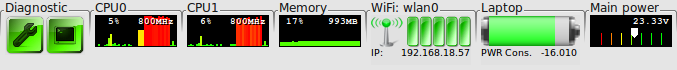
\includegraphics[width=13cm]{../../Common/img/ros/elektron_dashboard}
\caption[Okno interfejsu diagnostycznego]{Okno interfejsu diagnostycznego. W
kolejności od lewej: przywołanie okna wyświetlającego dokładne komunikaty z modułów diagnostycznych, przywołanie
konsoli z komunikatami systemu ROS, obciążenie procesora (dwa rdzenie), stan
pamięci RAM, poziom sygnału sieci bezprzewodowej, stan naładowania akumulatora
laptopa oraz napięcie na akumulatorach robota.}
\label{fig:elektron_dashboard}
\end{figure}
 
\cleardoublepage
% !TeX root = main.tex


\begin{savequote}[70mm]
,,Mapy mają dwie zasadnicze cechy: nie są terytorium, które opisują, ale, jeśli
są zrobione poprawnie, mają podobną do nich strukturę, co powoduje o~ich
przydatności.''
\qauthor{Alfred Korzybski}
\end{savequote}


\chapter{System nawigacji}
\label{chap:mapa}

\section{Struktura systemu nawigacji}

Wybór struktury programowej ROS pociągnął za sobą w~sposób naturalny kolejne
wybory związane ze strukturą systemu nawigacji robota. Zgodnie z~filozofią
twórców tego oprogramowania, podsystem nawigacji dla robota mobilnego podzielony
jest na kilka modułów, których wzajemna współpraca i~zależności pokazane są na
rysunku~\ref{fig:diag_move_base}. Część z~nich jest dostarczana razem z~systemem
ROS i~wykorzystywana bez zmian w~kodzie (of the shelf), niektóre mogą być
swobodnie wymieniane pod warunkiem, że spełniają wymogi odpowiednich interfejsów
(razem z~systemem dostarczone są pewne implementacje, z~których można
skorzystać), wymagane jest też dostarczenie kilku modułów zależnych od samego
robota, na którym całość jest uruchamiana.

\begin{figure}[h!]
\centering
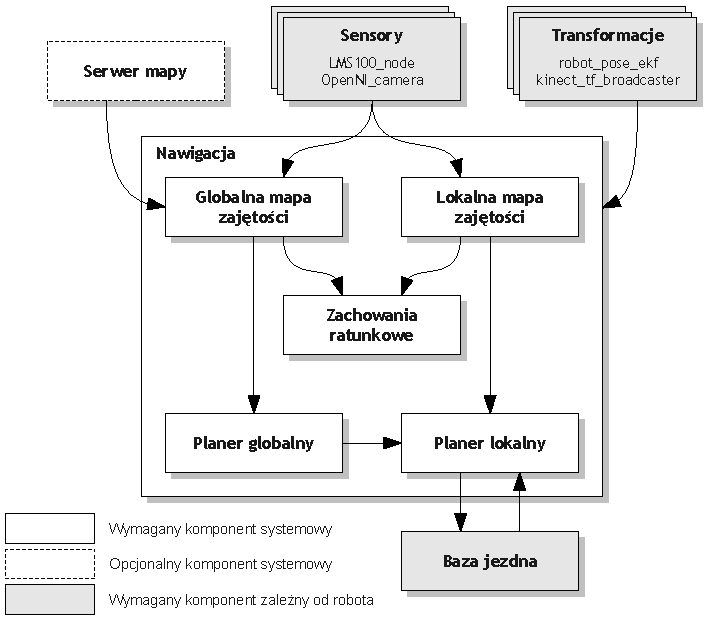
\includegraphics{../img/diag_move_base}
\caption{Struktura systemu nawigacji robota}
\label{fig:diag_move_base}
\end{figure}

Modułami, które są dostarczone i~niezmienne są mapy przeszkód (konkretnie
moduły agregujące dane z~sensorów i~tworzące na ich podstawie mapy zajętości).
Modułami wymiennymi są planery trasy (zarówno lokalny jak i~globalny) oraz
zachowania awaryjne mające na celu wyprowadzenie robota z~trudnych sytuacji
(np. otoczenie przeszkodami). Dodatkowo wymagane jest dostarczenie przynajmniej
modułów sensorycznych, modułów określających lokalizację robota w~pewnym,
globalnym układzie współrzędnych (może to być układ związany z~punktem startowym
robota) oraz oczywiście głównego sterownika robota. Ogólnie cały system można
podzielić na trzy główne części, odpowiedzialne za wykrywanie przeszkód 
i~tworzenie lokalnych map zajętości (kosztu), lokalizację robota oraz planowanie
trasy (globalne i~lokalne).

\section{Tworzenie map przeszkód}

Podczas poruszania się robota w~środowisku o~nie w~pełni znanej strukturze
kluczowe jest wykrywanie aktualnej konfiguracji przeszkód. W~środowiskach
statycznych wystarczy samo ich zaznaczanie na mapie, w~przypadku otoczenia
dynamicznie się zmieniającego równie ważne jest wykrywanie momentów, w~których
przeszkody znikają (czyszczenie przeszkód na mapie jest trudniejsze niż ich
oznaczanie). Cały proces wykrywania i~oznaczania przeszkód można podzielić na
cztery etapy:

\begin{itemize}
  \item agregacja danych z~sensorów,
  \item filtrowanie danych,
  \item oznaczanie przeszkód w~pewnej, wybranej strukturze danych,
  \item tworzenie dwuwymiarowej mapy kosztu.
\end{itemize}

\subsection{Agregacja danych z~czujników}

Pierwszym etapem jest zebranie danych z~sensorów. W~przypadku robota Elektron
istnieją dwa źródła danych o~przeszkodach -- skaner laserowy SICK oraz sensor
Kinect. Biorąc pod uwagę wielkość otrzymywanych danych (w~przypadku lasera
kilkaset punktów, w~przypadku sensora Kinect kilka tysięcy na każdy pomiar) oraz
stosunkowo niewielką prędkość poruszania się robota, do wykrywania przeszkód
nie są wykorzystywane wszystkie odczyty, a~jedynie pięć na sekundę w~przypadku
lasera oraz dwa na sekundę w~przypadku Kinecta.

Po zebraniu pomiarów muszą one jeszcze zostać przetransformowane do wspólnego
układu współrzędnych, w~tym przypadku do układu związanego z~bazą robota 
(w~przypadku sensora Kinect należy także wziąć pod uwagę jego pochylenie względem
bazy). Za publikację wszystkich niezbędnych transformacji  odpowiedzialne są
komponenty \comp{kinect\_tf\_broadcaster} oraz \comp{laser\_tf}.

\subsection{Filtrowanie danych}

Dane odebrane z~sensorów podlegają dalszemu procesowi filtracji, który ma na
celu usunięcie odczytów w~jakikolwiek sposób zafałszowanych. Odczyty ze skanera
laserowego są obarczone takimi błędami w~sposób niewielki, dlatego w~tym
przypadku filtracja się nie odbywa. Inaczej przedstawia się kwestia odczytów 
z~Kinecta -- pojawiające się w~nich pojedyncze, przypadkowe punkty mogą powodować
pojawianie się na mapie przeszkód uniemożliwiających ruch robota. Z tego powodu
stosowana jest filtracja danych ze względu na otoczenie punktów -- pojedyncze
odczyty, odstające od reszty pomiarów (posiadające w~otoczeniu zbyt mało
sąsiadów) są odrzucane.

\subsection{Mapa wokselowa}

Wszystkie punkty, które przejdą przez proces filtracji, są przekazywane do
modułu tworzącego mapę zajętości. Wewnętrznie przechowuje on reprezentację
otoczenia w~postaci mapy wokselowej (trójwymiarowa siatka prostopadłościanów).
Zmieniając wielkość oczek siatki możemy wybierać pomiędzy dokładnością pokrycia
otoczenia (im większe oczka, tym przeszkody będą zajmowały więcej miejsca, nawet małe
przeszkody będą reprezentowane przez całe zajęte oczka siatki) a~szybkością
działania i~obciążeniem systemu (małe oczka wymagają dużo większego nakładu
obliczeniowego). Implementacja dostępna w~systemie ROS ze względów
optymalizacyjnych zakłada maksymalnie 16 poziomów siatki w~pionie, nie jest to
jednak ograniczenie w~sposób szczególny wpływające na jej użyteczność. Dzięki
przyjętemu sposobowi reprezentacji (każda kolumna w~mapie reprezentowana przy
pomocy jednej liczby całkowitej) można było natomiast zastosować wydajne
algorytmy śledzenia promieni (wykorzystywane przy czyszczeniu przeszkód z~mapy).

Największym ograniczeniem tej struktury danych jest założenie, że robot porusza
się po płaskim terenie, na którym nie występują spadki (np. schody w~dół), przez
co przeszkody o~,,ujemnej wysokości'' nie są w~żaden sposób wykrywane. Niestety,
moduł odpowiedzialny za tworzenie map otoczenia nie jest przystosowany do
łatwego dostarczania własnych implementacji wewnętrznych struktur danych 
i~algorytmów (tak jak np. planery trasy). Istniały dwie możliwości
rozwiązania tego problemu: stworzenie kopii dużej części systemu i~wprowadzanie
w~niej własnych zmian, bądź napisanie modułu pośredniczącego pomiędzy sensorem 
a~algorytmami oznaczania przeszkód, która to metoda została wybrana.

\begin{figure}[htb!]
\centering

\includegraphics{../img/filtering}
\caption{Potok przetwarzania chmury punktów z~sensora Kinect}
\label{fig:filtering}
\end{figure}

\subsubsection{Wykrywanie spadków terenu}

Przed przekazaniem danych z~sensora Kinect do dalszych algorytmów tworzenia map
przeszkód są one przetwarzane przez zestaw filtrów. Pierwszy z~nich usuwa punkty
odstające w~pewien sposób od reszty pomiaru, a~więc takie, które mogą sugerować
szum pomiarowy. Punkty te są wykrywane przez zliczanie sąsiadów w~ich otoczeniu
o~określonej wielkości, a~jeśli tych sąsiadów będzie mniej niż dwóch, punkt taki
jest odrzucany z~dalszych obliczeń.

\begin{figure}[htb!]
\centering
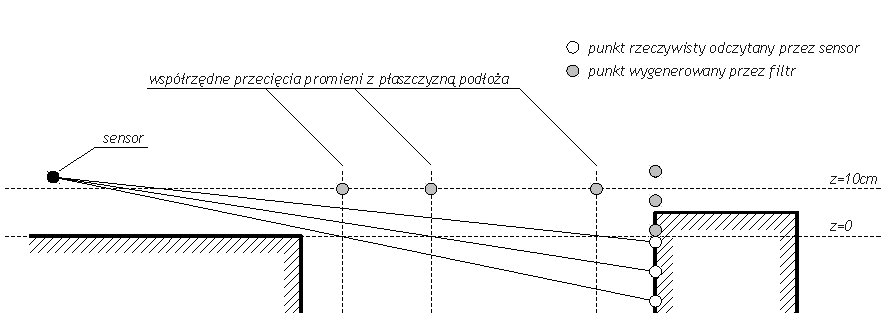
\includegraphics{../../Common/img/depresion}
\caption{Wykrywanie spadków terenu}
\label{fig:depresion}
\end{figure}

Kluczowym filtrem jest jednak wykrywanie spadków terenu. Zostało ono zrealizowane
w~sposób koncepcyjnie dość prosty, dający jednak bardzo dobre rezultaty. Dla punktów
o~współrzędnej $z>0$ wykonywane
jest proste przepisanie bez żadnych zmian, natomiast punkty poniżej progu są przekazywane
do dalszej obróbki. W~pierwszym kroku są one odbijane względem płaszczyzny $z=0$
(a więc punkt o~współrzędnych $(x, y, z)$ zamieniany jest na punkt o~współrzędnych
$(x, y, -z)$). Jako, że zazwyczaj wykrywane są przeszkody dopiero w~pewnej
odległości od spadku terenu (patrz rysunek~\ref{fig:depresion}), konieczne jest
znalezienie właściwego miejsca spadku. W~tym celu wyznaczane jest równanie prostej
łączącej aktualnie badany punkt ze środkiem sensora, a~z niego wyliczane są współrzędne
$x$ oraz $y$ miejsca przecięcia tej prostej z~płaszczyzną $z=0$. Do chmury dodawane
są dodatkowe punkty o~współrzędnych $x$ i~$y$ wyliczonych wcześniej oraz współrzędnej
$z=0.1$ (symulowana jest przeszkoda znajdująca się 10cm ponad poziomem podłoża).
W ten sposób lokalny planer trasy jest niejako zmuszany do omijania spadków terenu.

\subsubsection{Czyszczenie przeszkód}

Pierwszym krokiem po dostarczeniu przetworzonej wstępnie chmury punktów do algorytmu
oznaczającego przeszkody jest oczyszczenie mapy z~przeszkód, które nie są już widoczne.
Dla każdego punktu z~danego pomiaru wykonywany jest ten sam algorytm. Pomiędzy
bieżącym punktem a~środkiem sensora z~którego pochodzi dany pomiar prowadzony jest
odcinek prostej, a~każda komórka mapy, przez który dany odcinek przechodzi jest
czyszczona z~przeszkód. Jako, że mapa jest dyskretna i~ma stosunkowo duże oczka,
do wyznaczania kolejnych komórek przez które przechodzi bieżący promień wykorzystany
został algorytm Bresenhama (rozszerzony na przypadek trójwymiarowy). Ogólnie czyszczenie
przeszkód z~mapy jest zadaniem dość czasochłonnym, widać też, że w~przyjętym algorytmie
do wyczyszczenia nieistniejących przeszkód konieczne jest istnienie innej przeszkody
tak, aby odpowiednie punkty pojawiły się w~chmurze z~pomiaru (jeśli nie będzie możliwości
poprowadzenia promienia przez dany punkt z~powodu braku odpowiednich pomiarów, to
przeszkoda taka nie zniknie z~mapy). Własność ta sprawia, że tworzenie lokalnych
map zajętości o~zbyt dużych rozmiarach może spowodować problemy (przypadkowe przeszkody
pojawiające się w~otwartym terenie daleko od robota mogą nigdy nie zostać wyczyszczone).

\subsubsection{Oznaczanie przeszkód}

Oznaczanie przeszkód wykonywane po oczyszczeniu poprzedniego stanu mapy jest zadaniem
dużo prostszym, zarówno koncepcyjnie jak i~obliczeniowo. Dla każdego punktu z~danego
pomiaru wyznaczana jest komórka, w~której dany punkt leży, a~następnie jest ona
oznaczana jako zajęta.

Kolejność wykonywanych działań, a~więc najpierw czyszczenie, a~dopiero potem
oznaczanie nowych przeszkód ma kluczowe znaczenie. Gdyby wykonywane było jednocześnie
dla każdego punktu i~czyszczenie, i~oznaczanie przeszkód, mogłoby dochodzić do
sytuacji, w~których dopiero co oznaczone w~mapie obiekty byłyby usuwane przez proces
czyszczenia wywoływany dla innych punktów z~danego pomiaru.


\subsection{Mapa zajętości}

Po zaznaczeniu wszystkich przeszkód w~mapie wokselowej, są one rzutowane na
dwuwymiarową mapę zajętości. Wszystkie kolumny, w~których są oznaczone zajęte
komórki są oznaczane jako zajęte, jeśli natomiast w~kolumnie są tylko komórki
puste bądź nieznane, to w~zależności od ilości nieznanych oznaczenie jest różne.
Jeśli więcej niż 4 komórki są nieznane, wtedy cała kolumna jest uznawana za
nieznaną, w~przeciwnym wypadku kolumna jest uznawana za pustą.

Po oznaczeniu przeszkód dokonywane jest ich powiększenie na określoną odległość
(nadmuchiwanie). Operacja ta ma na celu wygładzenie mapy kosztu i~spowodowanie,
że robot nie będzie preferował szerokie przejazdy (o ile będzie miał wybór). NA
rysunku~\ref{fig:inflation} przedstawiona jest ogólna metoda obliczania kosztu
dla komórki podczas tego procesu. Parametrem kontrolującym ten proces jest
promień ,,nadmuchiwania'', od którego zależy, jak dużą odległość od
przeszkód będzie zachowywał robot.

\begin{figure}[htb!]
\centering
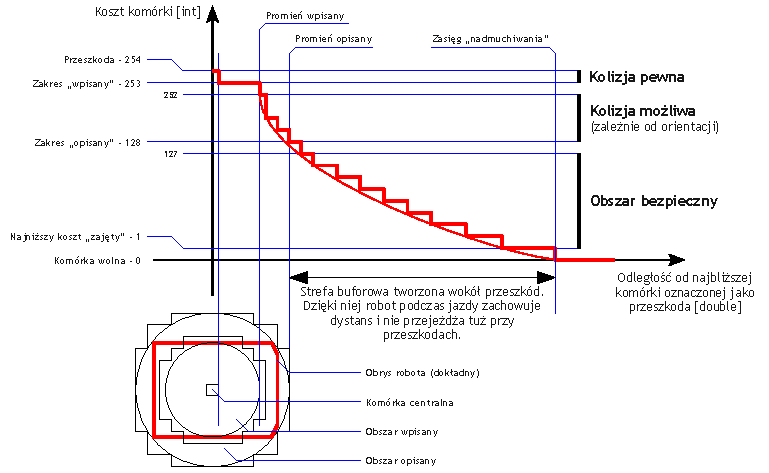
\includegraphics[width=15cm]{../../Common/img/ros/inflate.pdf}
\caption{Nadmuchiwanie przeszkód.}
\label{fig:inflation}
\end{figure}

Mapa zajętości ma stały rozmiar, a~jej środek związany jest ze środkiem bazy
jezdnej robota. W~środowiskach o~dynamicznie zmieniającej się konfiguracji
przeszkód przechowywanie globalnej mapy zajętości (innej niż statyczna mapa
otoczenia) często powoduje więcej problemów niż pożytku -- przeszkody widoczne
na niej w~dużej odległości od robota mogą faktycznie już zniknąć, a~pozostając
na mapie mogą zakłamywać globalne planowanie ścieżki. Dodatkowo wprowadzona jest
duża oszczędność pamięci, gdyż przechowywana mapa ma stały rozmiar, niezależnie
od przejechanego przez robota dystansu i~wielkości eksplorowanego środowiska.

\section{Lokalizacja robota}

Obliczanie względnej pozycji robota (a więc liczona na podstawie jego ruchu, względem
punktu początkowego) zostało opisane już wcześniej przy okazji opisu odometrii
oraz rozszerzonego filtru Kalmana. W~przypadku aplikacji, gdzie nie jest wykorzystywany
żaden system lokalizacji globalnej jest to jedyne źródło informacji o~położeniu,
użytkownik może dodatkowo wskazać na mapie położenie początkowe aby umożliwić pracę
globalnego planera trasy.

Możliwe jest także zastosowanie algorytmu globalnej lokalizacji -- jest to element
wymienny w~systemie nawigacji i~może być tam zastosowany dowolny gotowy bądź zaimplementowany
w~ramach badań algorytm. Jest to więc jeden z~elementów, które mogą być testowane
przy użyciu stworzonej platformy badawczej -- sama wymiana modułu lokalizacji jest
bardzo łatwa i~sprowadza się jedynie do uruchomienia własnego procesu z~algorytmem
w~miejsce istniejącego. W~szczególności jako algorytm lokalizacji globalnej może być
podany program wykorzystujący jedynie odometrię (tak jak zostało to opisane w~poprzednim
akapicie).

Do celów globalnego wyznaczania trasy oraz ewentualnej globalnej lokalizacji stworzona
została mapa kilku pomieszczeń, po których poruszał się robot. Jej tworzenie było
dwuetapowe -- najpierw przy pomocy algorytmu SLAM i~skanera laserowego zostały
stworzone mapy poszczególnych pomieszczeń (w~kilku częściach, ze względu na możliwości
obliczeniowe komputera sterującego). Mapy te zawierały oczywiście wszystkie bieżące
przeszkody i~ruchome elementy wyposażenia, takie jak stoły, krzesła czy pudła.
Na podstawie tych map stworzona została ręcznie w~programie typu CAD oczyszczona
mapa, zawierająca jedynie ściany pomieszczeń, duże meble (takie, których przestawienie
nie jest w~łatwy sposób możliwe, a~więc szafy pancerne i~ciężkie biurka warsztatowe)
oraz niedostępny dla robotów mobilnych podest z~manipulatorami. Wszystkie pozostałe
elementy (w~szczególności mniejsze stoły, krzesła czy kosze na śmieci) zostały z~tej
mapy usunięte.

W przygotowanych aplikacjach jako do nawigacji globalnej (względem dostarczonej
zgrubnej mapy środowiska) został wykorzystany algorytm AMCL (Adaptive Monte Carlo
Localization~\cite{fox2001kld}) wykorzystujący filtr cząsteczkowy do śledzenia
pozycji robota na znanej mapie. Pozycja jest wyznaczana na podstawie odczytów
ze skanera laserowego oraz z~układu odometrii robota. Ważne jest to, że pojawiające
się wokół robota przeszkody, które nie są umieszczone na mapie, nie wpływają znacząco
na jakość lokalizacji (dopóki robot przez dłuższy czas nie będzie nimi całkowicie
otoczony), oraz że algorytm szybko odnajduje właściwe położenie robota po jego
chwilowym zagubieniu. Algorytm bardzo dobrze radzi sobie z~lokalizowaniem robota nawet
posiadając jedynie zgrubną mapę otoczenia zawierającą kluczowe cechy otoczenia
(opisaną wcześniej).

\section{Planowanie trasy}

\subsection{Ścieżka globalna}

Po wskazaniu punktu docelowego uruchamiany jest globalny planer trasy. Element ten
jest wymienny i~może być wykorzystana implementacja dowolnego algorytmu (spełniająca
warunki narzucone przez interfejs systemu), tak więc jest to kolejny element, na którym
mogą być przeprowadzane eksperymenty używając stworzonej platformy. W~aplikacjach
testowych został wykorzystany algorytm Dijkstry wyszukiwania ścieżki w~grafie tworzonym
na podstawie mapy globalnej. Początkowo uwzględniana jest jedynie sama mapa, bez
dodatkowej informacji o~przeszkodach, a~w momencie, kiedy robot nie zdoła wykonać
zadanego planu, algorytm uruchamiany jest ponownie uwzględniając już przeszkody
z~dynamicznie tworzonej mapy zajętości wokół robota (które w~szczególności mogą
przesłaniać niektóre przejazdy, np. zamknięte drzwi).

Planer globalny wprowadza dodatkowe założenia o~kształcie robota -- przyjmuje, że
jest on okrągły i~do obliczeń wykorzystuje okrąg opisany na faktycznym obrysie robota.
Wynikają z~tego drobne problemy tego podejścia, mianowicie może się okazać, że nie
zostanie wyznaczona żadna ścieżka mimo, iż w~przy pewnej konfiguracji robot zmieściłby
się pomiędzy przeszkodami (np. przejeżdżając ,,na styk'' pomiędzy nimi). Sytuacja
taka nie wystąpiła jednak w~czasie eksperymentów, a~kształt robota Elektron jest
na tyle zwarty, że dla celów globalnego planowania trasy może być przybliżony okręgiem.

\subsection{Ścieżka lokalna}

Po wyznaczeniu planu globalnego jego fragmenty są przesyłane do lokalnego planera
trasy działającego z~wykorzystaniem algorytmu okna dynamicznego (opisany 
w~rozdziale~\ref{chap:nawigacja}). Obliczenia wykorzystują lokalną mapę zajętości
tworzoną wokół robota (z nanoszonymi na nią na bieżąco przeszkodami) oraz
bieżące odczyty z~układu odometrii robota (aktualna prędkość).
Funkcja liczenia kosztu ruchu jest ustawiona tak,
aby najmniejszym kosztem obarczone były trajektorie kończące się blisko ścieżki globalnej,
natomiast odjeżdżanie od niej owocowało zwiększaniem kosztu. Dużym problemem okazało
się dobranie odpowiednich parametrów algorytmu (a więc ograniczeń na prędkości
oraz długości pojedynczego kroku czasowego symulacji). Przy zbyt długim kroku
algorytm często wybierał ruch obrotowy z~niewielką prędkością liniową, który skutkował
powrotem do punktu wyjścia (koszt takiego ruchu był minimalny, gdyż kończył się dokładnie
na wyznaczonej ścieżce). Po eksperymentach i~ustawieniu parametrów robot wykonywał
wyznaczone ścieżki z~dużą szybkością (ok. 15cm/s, a~więc 75\% maksymalnej prędkości
dozwolonej dla robota) sprawnie unikając pojawiających się przeszkód.

\cleardoublepage
% !TeX root = main.tex


\begin{savequote}[70mm]
,,--No, dobrze -- powiedział Puchatek -- a gdybym ja posadził plaster miodu przed moim domem, czy wyrośnie z niego ul?''
\qauthor{Alan Alexander Milne}
\end{savequote}


\chapter{Aplikacje i~testy}
\label{chap:aplikacje}

\section{Automatyczna kalibracja odometrii i~żyroskopu}

Proces kalibracji odometrii oraz pomiarów uzyskiwanych z~żyroskopu został
przestawiony w~rozdziale~\ref{chap:software}. W~celu jego ułatwienia
i~zautomatyzowania stworzona została aplikacja przeprowadzająca dwuetapową
kalibrację -- najpierw wyliczająca poprawki dla współczynników kątowych
żyroskopu i~odometrii, a~następnie licząca poprawkę dla składnika liniowego
odometrii. Aby poprawnie przeprowadzić cały proces wymagana jest pusta
przestrzeń o~powierzchni ok. 2x2m, oraz płaska powierzchnia na jednym z~końców
(np. ściana).

\subsection{Wyznaczanie odległości i~kąta obrotu względem ściany}

W celu wyznaczenia faktycznej wartości obrotu wykonanego przez robota oraz
określenia pokonanej odległości, wymagana jest obecność sensora zwracającego
odczyty laserowe (w~przypadku robota Elektron możliwe jest wykorzystanie
zarówno skanera SICK jak i~sensora Kinect z~dodatkowym komponentem
zamieniającym pomiary z~chmury punktów na symulację odczytu laserowego). Na
podstawie punktów zwracanych przez sensor ustawiony na przeciwko ściany
wyliczana jest orientacja robota względem niej, a~także odległość.

\subsubsection{Orientacja}

Dane odczytane z~lasera mają postać zbioru punktów we współrzędnych biegunowych.
Pierwszym krokiem jest ich przeliczenie na współrzędne kartezjańskie w~układzie
związanym ze środkiem sensora. Po takim przeliczeniu, wykorzystując metodę
najmniejszych kwadratów, wyliczane są parametry prostej przechodzącej możliwie
blisko danych punktów. Współczynnik kierunkowy tej prostej określa jednocześnie
orientację robota względem ściany.

Mając dane punkty w~postaci $(x_i, y_i)$, gdzie $i=1\ldots n$, oraz przyjmując
oznaczenia:

\[
S_x = \sum_{i=1}^n x_i \mathsp
S_y = \sum_{i=1}^n y_i \mathsp
S_{xx} = \sum_{i=1}^n x_i^2 \mathsp
S_{xy} = \sum_{i=1}^n x_i \cdot y_i \mathsp
%S_{yy} = \sum_{i=1}^n y_i^2 \mathsp
\Delta = n \cdot S_{xx} - S_x^2
\]

Współczynniki prostej o~równaniu $y=a\cdot x+b$ wyznaczane są przez wzory:

\[
a~= \frac{n \cdot S_{xy} - S_x \cdot S_y}{\Delta} \mathsp
b = \frac{S_{xx} \cdot S_y - S_x \cdot S_{xy}}{\Delta}
\]

Skąd orientację robota względem ściany (wyznaczonej prostej) uzyskujemy ze
wzoru:

\[
\phi=atan(a)
\]

\subsubsection{Odległość}

Wykorzystując już punkty we współrzędnych kartezjańskich, odległość od ściany
wyliczana jest jako średnia z~wartości $y$ wszystkich punktów.

\subsection{Właściwy proces kalibracji}

Przed rozpoczęciem kalibracji robot powinien zostać ustawiony na wprost ściany,
w~odległości ok. 50cm od niej. Pierwszą czynnością po uruchomieniu zadania jest
wyznaczenie składowej stałej pomiarów z~żyroskopu, po czym następują trzy
pełne obroty robota z~różnymi prędkościami (fakt wykonania pełnego obrotu
wyznaczany jest na podstawie odczytów z~odometrii). Po wykonaniu każdego obrotu
wyliczana jest faktyczna jego wartość (na podstawie porównania orientacji
względem ściany zmierzonej przed i~po wykonaniu obrotu), a~razem z~nią
zapamiętywane są wartości obrotu odczytane z~odometrii i~żyroskopu. Pomiędzy
kolejnymi pomiarami robot jest pozycjonowany powtórnie na wprost ściany
(z~pewną, niewielką tolerancją) wykorzystując pomiary laserowe. Po wykonaniu
wszystkich obrotów wyliczane są błędy wskazań odometrii i~żyroskopu (stosunek
wartości odczytanej do zmierzonej laserem), a~z nich wyliczana jest średnia
wartość poprawki, którą należy wprowadzić do współczynników obrotowych obu
badanych czujników.

Po wykonaniu kalibracji obrotów robot powtórnie ustawia się na wprost ściany,
a~następnie odjeżdża od niej na odległość ok. 2 metrów. Następnie przejeżdża 1.5
metra do przodu, a~po przejechaniu tego dystansu wyliczana jest poprawka
współczynnika liniowego odometrii (stosunek przejechanej odległości wyliczonej
przez odometrię do odległości uzyskanej z~pomiarów laserowych). Ostateczna
wartość poprawki wyliczana jest jako średnia z~trzech takich przejazdów
z~różnymi prędkościami. Uzyskane w~tym procesie wartości współczynników należy
pomnożyć przez współczynniki już ustawione w~sterownikach robota.



\section{Prosta, losowa eksploracja}

Kolejną aplikacją, która powstała w~celu przetestowania poprawnego działania
sensorów oraz sterownika silników była losowa eksploracja terenu. Podczas
ruchu wyznaczana jest minimalna odległość do przeszkód w~dwóch strefach
-- po lewej oraz prawej stronie. Jeśli wokół robota nie ma przeszkód bliżej,
niż ustalona odległość minimalna, to porusza się on na wprost. W~przeciwnym
wypadku prędkość kątowa jest proporcjonalna do różnicy odległości przeszkód
po lewej i~prawej stronie (o kierunku takim, aby dążyć do wyrównania odległości
po obu stronach), a~prędkość liniowa proporcjonalna jest do średniej odległości
przeszkód po obu stronach.

Zadanie spełnia swoją podstawową rolę -- pozwala na przetestowanie różnych
zestawów sensorycznych (skanera laserowego, Kinecta) oraz zweryfikowanie
poprawności działania układu zarządzającego pracą silników. Niestety, ze względu
na bardzo prosty algorytm zastosowany do omijania przeszkód, zdarzają się sytuacje
blokady robota w~narożnikach pomieszczeń (średnia odległość od przeszkód po
obu stronach jest taka sama, więc robot nie skręca, a~ściany są na tyle blisko,
że prędkość liniowa została wyzerowana). Innym pojawiającym się problemem
jest wjeżdżanie w~przeszkody podczas zakręcania przy korzystaniu z~sensorów
o~dużej minimalnej odległości działania i~wąskim polu widzenia. Spowodowane jest
to brakiem jakiejkolwiek pamięci co do przeszkód (np. małej lokalnej mapy zajętości),
przez co jeśli robot stoi obok ściany (której nie wykrywa czujnikami, bo nie jest
w~ich polu widzenia) i~odwróci się w~jej stronę, to może na nią wjechać (czujniki
nie wykryją przeszkody, gdyż znajduje się ona zbyt blisko).



%\section{Budowa mapy}



\section{Dojazd do wyznaczonego celu z~omijaniem przeszkód}

Ostatnią, a~zarazem kluczową aplikacją stworzoną w~ramach tej pracy jest
pełny system nawigacji (o strukturze opisanej w~poprzednich rozdziałach)
przygotowany do możliwie maksymalnego wykorzystania wszystkich dostępnych
elementów (tj. układów sensorycznych, systemów lokalizacji). Eksperymenty
przeprowadzane były w~laboratorium robotyki i~jego okolicach, a~więc w~pomieszczeniach
o~charakterze biurowo-warsztatowym, z~wieloma obiektami przenoszonymi z~miejsca
na miejsce. Szczególnie często na korytarzu zmieniała się konfiguracja przeszkód
-- przestawiane krzesła, drzwi otwierane czasami częściowo, czasami całkowicie,
a~także przechodzący ludzie. Zgodnie z~założeniami zadania, robot miał poradzić
sobie w~takim środowisku i~dążyć do osiągnięcia zadanego celu.

\subsection{Scenariusz pracy}

Scenariusz działań podczas korzystania z~tej aplikacji jest dość prosty -- początkowo,
po uruchomieniu robota i~wszystkich niezbędnych modułów opisanych wcześniej, należy
wskazać jego przybliżoną pozycję i~orientację na mapie. Następnym krokiem jest
wskazanie punktu docelowego, który robot ma osiągnąć. W~zależności od jego osiągalności,
a~w~zasadzie tego, czy planer globalny będzie w~stanie wyznaczyć prawidłowy plan
czy nie, podejmowane są różne akcje. Jeśli plan nie zostanie odnaleziony, to wyświetlany
jest odpowiedni komunikat oraz emitowany dźwięk oznaczający niepowodzenie wykonania
zadania. Jeśli ścieżka zostanie wyznaczona, emitowany jest dźwięk akceptacji celu
i~rozpoczyna się wykonanie trajektorii, segment po segmencie. Podczas jazdy może się
okazać, że wyznaczona ścieżka jest niemożliwa do wykonania (np. zostały zamknięte
drzwi, przez które wiodła trajektoria), robot się zatrzymuje i~uruchamiany jest
ponownie planer globalny (z dodatkową wiedzą o~stanie przeszkód w~okolicy robota).
Po dojechaniu do wyznaczonego celu (z pewną, określaną z~góry dokładnością zarówno
co do położenia jak i~orientacji) robot zatrzymuje się i~emitowana jest informacja
o~poprawnym wykonaniu zadania.

\subsection{Obsługa sytuacji wyjątkowych}

Odrębnym przypadkiem jest próba wybrnięcia z~sytuacji wyjątkowych, w~których mógł się
znaleźć robot. Do sytuacji takich należy przede wszystkim okrążenie przeszkodami.
Jest to stosunkowo częsta sytuacja, szczególnie że czujniki na robocie nie rejestrują
pełnego otoczenia, a~jedynie jego fragment przed robotem oraz ewentualnie po bokach.
Jeśli przed robotem stanie człowiek, robot się odwróci, a~obraz przeszkody pozostanie
na jego lokalnej mapie zajętości. Jeśli w~ten sposób robot zostanie na chwilę okrążony,
to pomimo faktycznego zniknięcia tych obiektów, stanowią one przeszkodę dla algorytmu
wyznaczania ścieżki lokalnej i~sygnalizuje on zakleszczenie. W~tym momencie uruchamiane
są zachowania mające na celu wyprowadzenie robota z~tego stanu i~oczyszczenie mapy
zajętości.

W przygotowanym systemie sterowania zachowania te są możliwe do łatwej zmiany, pozwalając
na eksperymenty z~różnego rodzaju mniej i~bardziej agresywnymi podejściami. W~stworzonej
aplikacji wykorzystane zostały dwa domyślne podejścia. Pierwsze z~nich po zatrzymaniu
robota czyści przeszkody znajdujące się dalej niż ustalony limit od robota. Drugie
wykonuje obrót w~miejscu o~360\textdegree~wypełniając mapę aktualnymi informacjami
o~środowisku wokół. Po uruchomieniu każdego z~zachowań ratunkowych sprawdzane jest,
czy możliwe jest kontynuowanie jazdy, w~przeciwnym wypadku uruchamiane jest kolejne
zachowanie, aż do wyczerpania wszystkich dostępnych możliwości. W~takim wypadku
emitowana jest informacja o~niepowodzeniu zadania. Graf przedstawiający kolejność
uruchamiania zachowań ratunkowych przedstawiony jest na rysunku~\ref{fig:recovery}.

\begin{figure}[h!]
\centering
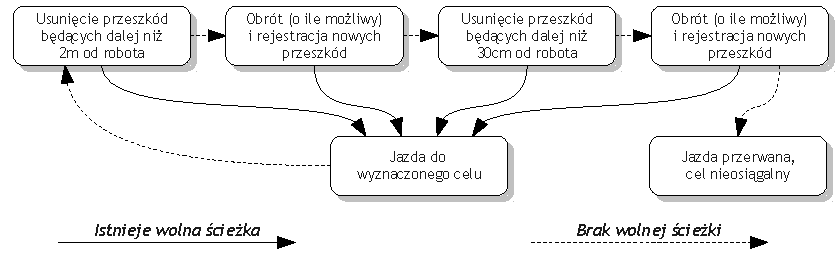
\includegraphics[width=\textwidth]{../img/recovery}
\caption{Diagram stanu wyboru zachowań ratunkowych}
\label{fig:recovery}
\end{figure}

\section{Weryfikacja poprawności działania}

Największym problemem w~aplikacjach robotycznych jest weryfikacja poprawności ich
działania. Możliwe jest napisanie testów jednostkowych samego oprogramowania,
nie da się jednak stworzyć podobnych testów dla aplikacji wykorzystujących sprzęt
taki jak roboty. Istnieje kilka podejść przeprowadzania testów mających na celu
zwiększenie prawdopodobieństwa działania aplikacji zgodnie z~oczekiwaniami.
Pierwszą metodą jest wykorzystanie symulatorów (zarówno ogólnodostępnych, jak
i~specjalizowanych przygotowywanych specjalnie dla jednego robota). Kolejnym sposobem
jest przetestowanie aplikacji z~wykorzystaniem właściwego robota w~kontrolowanych
warunkach (z zachowaniem odpowiednich środków ostrożności). Istotne jest to, że
obie te metody można wykorzystać jednocześnie, sprawdzając najpierw ogólną poprawność
algorytmu na symulacji, a~następnie sprawdzając wszystkie możliwe przypadki użycia
(a przynajmniej tyle, ile można przewidzieć).

\subsection{Wykorzystanie symulacji}

Obecnie istnieje wiele gotowych symulatorów do testowania zachowań robotów
mobilnych, występują zarówno w~wersjach dwuwymiarowych (Stage) jak i~trójwymiarowych
(Gazebo). Posiadają możliwość pełnej symulacji układu robotycznego, zarówno
jego bazy jezdnej jak i~wielu różnych sensorów. Dodatkowo wyposażone są
w~moduł symulacji fizycznej, dzięki czemu symulacje mogą odwzorowywać dodatkowe
czynniki, takie jak różne współczynniki tarcia podłoża czy zderzenia.
Niestety, wielu elementów nie da się dokładnie zasymulować, chociażby ze
względu na występujące niedokładności rzeczywistych czujników, często o~charakterze
losowym i~różnego rodzaju szumy. Poza tym w~warunkach symulacji zazwyczaj dużo
lepiej działają wszystkie systemy lokalizacji.

\begin{figure}[htb!]
\centering
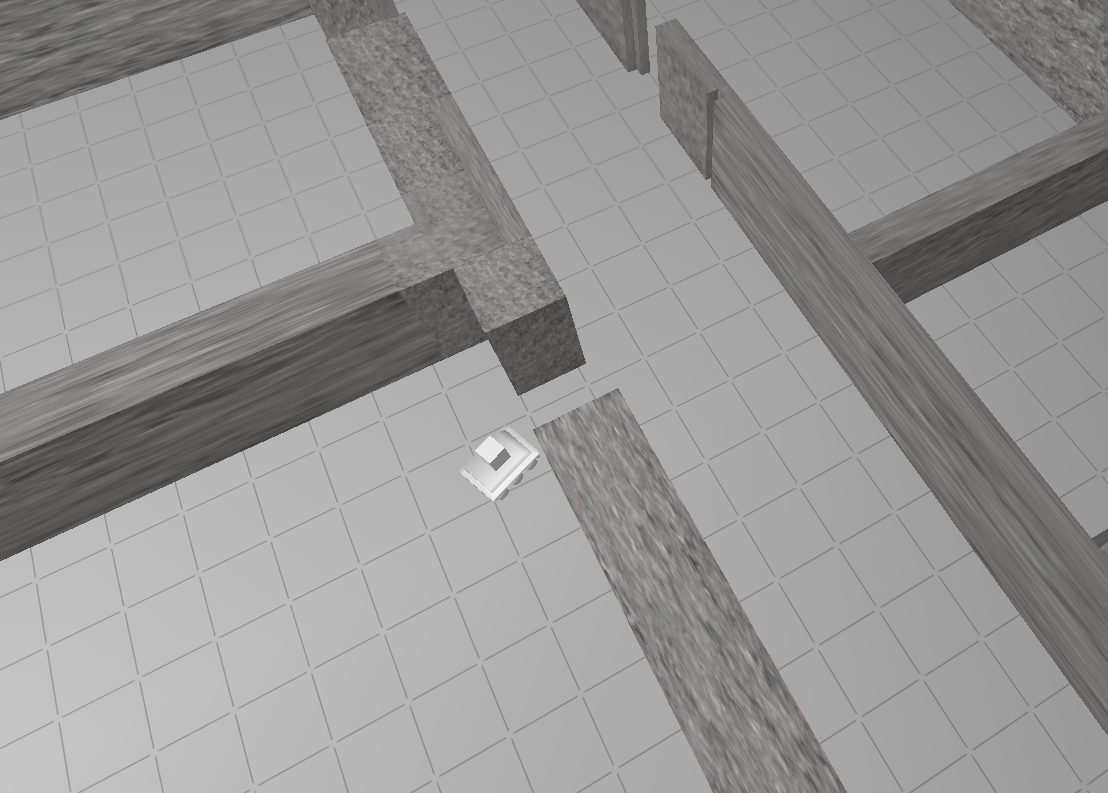
\includegraphics[width=13cm]{../img/gazebo}
\caption[Robot Elektron w symulatorze Gazebo]{Robot Elektron w symulatorze Gazebo.
Dodatkowo załadowany jedno ze środowisk dołączych do symulatora.}
\label{fig:gazebo}
\end{figure}

Mimo opisanych cech symulacji, jest to najlepsze narzędzie do przeprowadzania
wstępnych testów algorytmów sterowania. Nie ma ryzyka uszkodzenia sprzętu
przy wystąpieniu dużego błędu, można też zgrubnie dobrać wstępne wartości
parametrów różnych algorytmów. Podczas prac z~robotem Elektron wykorzystywany
był symulator Gazebo, wraz z~trójwymiarowym modelem robota i~prostym modelem
środowiska zawierającym kilka przeszkód (widok z~symulacji przedstawiony jest
na rysunku~\ref{fig:gazebo}). Podczas tych kilku pierwszych uruchomień
ustalone zostały takie parametry wielkości map i~dokładności różnych algorytmów,
aby nie występowało nadmierne obciążenie procesora na komputerze sterującym
robota.

\subsection{Testy w~kontrolowanych warunkach}

Po dobraniu wstępnych wartości dla algorytmów (zarówno lokalizacji jak
omijania przeszkód) rozpoczęły się testy na właściwym sprzęcie. Pierwsze
przejazdy odbywały się ze zmniejszoną prędkością, w~środowisku pozbawionym
przeszkód i~miały na celu sprawdzenie w~rzeczywistości poprawności pracy
wszystkich elementów nawigacji.

Pierwsze testy dotyczyły działania systemu lokalnej i~globalnej lokalizacji.
Po skalibrowaniu żyroskopu i~odometrii robot został ustawiony w~znanym położeniu
(oznaczonym później na mapie jako miejsce startowe) i~był sterowany przy pomocy
joysticka i~modułu teleoperacji. Podczas ruchu wykonywane były różne trajektorie,
m.in. jazda po prostej, zakręty o~różnym promieniu i~prędkości pokonywania
oraz nagłe zmiany szybkości ruchu. Podczas całego testu system lokalizacji
globalnej utrzymywał poprawne położenie robota w~odniesieniu do zgrubnej mapy
pomieszczenia, czasami jedynie gubiąc się w~długim korytarzu pozbawionym
cech charakterystycznych. System lokalizacji lokalnej po powrocie do punktu
startowego wykazywał różnicę zarówno w~położeniu jak i~orientacji, wartości
te wahały się od kilkunastu centymetrów przy krótkich trasach do nieco ponad
metra przy długich testach (wartość różnicy w~orientacji wynosiła maksymalnie 10\textdegree,
dokładniejsze dane dotyczące dokładności systemu lokalizacji lokalnej podane
są w~części dotyczącej rozszerzonego filtru Kalmana w rozdziale~\ref{chap:software}).

Kolejnym testowanym modułem był globalny planer trasy. Testy polegały na
wyznaczaniu robotowi różnych punktów docelowych, z~czego były możliwe
trzy sytuacje: punkt osiągalny bez dodatkowych warunków, punkt osiągalny
o~ile konfiguracja przeszkód na to pozwalała (w~tym przypadku zawsze pozwalała,
miało to znaczenie przy kolejnych testach, gdzie pojawiły się przeszkody)
oraz punkt nieosiągalny. W~każdym przypadku wykonano kilkanaście testów,
w~każdym przypadku trajektoria została wyznaczona prawidłowo i~robot wykonał
ją bez błędów, punkty docelowe nieosiągalne zostały wykryte i~odrzucone przez
algorytm wyznaczania trajektorii. W~tych samych testach sprawdzana była także
poprawność wykonywania trajektorii przez moduły planera trajektorii lokalnej.
Po dostrojeniu odpowiednich parametrów (głównie dotyczących w~tym przypadku
czasu planowania wprzód tak, aby uniknąć jazdy w~kółko) robot przeszedł
testy bezbłędnie (za każdym razem trajektoria lokalna śledziła globalną
bez kłopotów).

Po przetestowaniu zdolności śledzenia zadanej ścieżki testy przeniosły się
na moduł wykrywania i~omijania przeszkód. W~tym momencie kluczowe były dwie
kwestie: dokładne skalibrowanie chmury punktów uzyskiwanej z~sensora Kinect
tak, aby punkty odpowiadające podłodze leżały na płaszczyźnie o~równaniu
$z=0$, oraz ustawienie odpowiednich wartości dla wielkości oczka siatki
w~lokalnej mapie zajętości. Pierwsze zadanie wykonywane jest przed rozpoczęciem
jazdy przez robota przy użyciu małej aplikacji, która pozycjonuje Kinect
pod kątem 20\textdegree ~w dół, a~następnie odczytując dane z~wbudowanego
w~niego akcelerometru wyznacza faktyczne wartości kątów pochylenia i~skręcenia
używane przy przekształcaniu chmury z~układu związanego z~czujnikiem do układu
związanego z~robotem.

Dobór wielkości oczek lokalnej mapy zajętości miał kluczowe znaczenie przy zdolności
do pokonywania wąskich przejazdów przez robota. Przy zbyt dużej ich wielkości
przejazdy pomiędzy przeszkodami mogłyby stać się nieprzejezdne dla planera
ścieżki lokalnej, przy zbyt małej robot mógł zacząć wpadać na niektóre przeszkody
podczas wykonywania obrotów w~ich pobliżu, wzrosłoby też znacząco obciążenie
systemu. Wartość była dobierana eksperymentalnie w~taki sposób, aby robot był
w~stanie przejechać przez drzwi o~szerokości 80cm, pod możliwie wieloma kątami
(a więc nie tylko na wprost). Oczka o~wielkości 10cm okazały się zdecydowanie
zbyt mało dokładne, średnio w~70\% przypadków futryny po zaznaczeniu na mapie
znajdowały się w~odległości 60cm, a~po uwzględnieniu dodatkowej (dość niskiej,
bo jedynie 5cm) wartości dozwolonego dystansu od przeszkód okazywało się, że
robot nie jest w~stanie zmieścić się w~drzwiach (poprzez zmieszczenie się
rozumiana jest możliwość przejazdu przez drzwi oraz wykonania obrotu stojąc
pomiędzy futrynami). Siatka wielkości 5cm dużo dokładniej pokrywała przeszkody,
pozwalając na przejazd robota przez wąskie przesmyki. Niestety, z~powodu dodatkowego
obciążenia systemu konieczna stała się redukcja wielkości lokalnej mapy zajętości
z~początkowych dziewięciu do sześciu metrów (a więc po trzy metry od robota
w~każdą stronę).

Po kalibracji orientacji czujnika robot miał za zadanie pokonać trasy podobne,
jak przy poprzednich testach, tym razem mając na trasie ustawione dodatkowe
przeszkody (takie jak krzesła i~kartonowe pudełka). Planer trajektorii
globalnej wyznaczał oczywiście ścieżki nie uwzględniające ich, gdyż nie
były one zaznaczone na mapie, a~więc zadanie ich ominięcia spoczywało na
planerze lokalnym. Przy tym samym punkcie startowym i~docelowym oraz tej
samej konfiguracji przeszkód robot wykonał po 10 przejazdów w~obie strony
(od punktu startowego do docelowego i~z powrotem), z~czego w~dwóch przypadkach
nastąpił kontakt z~przeszkodą. Kontakt polegał na zahaczeniu podczas zakręcania
o~najbardziej wystające elementy podstawy fotela biurowego i~jego delikatne
przesunięcie, było to spowodowane małą wielkością oczka siatki w~mapie zajętości
i~dość wąskim polem widzenia sensora. Przeprowadzone zostały także testy
wykrywania sytuacji wyjątkowych opisanych wcześniej. Robot podczas ruchu
został otoczony przeszkodami (kartonowe pudła oraz ludzie) w~odległości
ok. metra. Początkowo algorytm wyznaczał ścieżkę omijającą przeszkodę przed
robotem, jednak wraz z~zakręcaniem wykrywane były kolejne, aż w~końcu wokół
całego robota na mapie zajętości pojawiły się przeszkody. W~tym momencie
robot się zatrzymał i~rozpoczął wykonywanie zachowań ratunkowych. Jeśli
w~tym czasie przeszkody zostały usunięte, robot kontynuował jazdę do celu,
jeśli natomiast pozostały na swoim miejscu, to po wykonaniu całej serii
wszystkich przewidzianych ruchów i~aktualizacji mapy zajętości robot sygnalizował
prawidłowo niemożność osiągnięcia celu.

Podczas testów z~przeszkodami zostało też sprawdzone wykrywanie nieprzejezdnych
obszarów (np. zamkniętych drzwi). Jeśli robot miał za zadanie przejechać pomiędzy
dwoma pomieszczeniami, gdzie przejazd możliwy był tylko przez jedne drzwi,
a~podczas przejazdu dojechał do zamkniętych drzwi, zatrzymywał się. W~tym
momencie uruchamiany był ponownie globalny planer trasy, który oczywiście
nie był w~stanie jej znaleźć i~sygnalizowany był błąd (punkt docelowy jest
nieosiągalny). Podobna sytuacja (zatrzymanie robota i~ponowne generowanie
ścieżki globalnej) występowała też podczas normalnego ruchu, kiedy istniało
kilka możliwych (z punktu widzenia dostarczonej mapy) dróg, a~wybrana okazywała
się nieprzejezdna (np. prowadziła przez obszar zastawiony krzesłami). W~tym
wypadku po ponownym wyliczeniu robot kontynuował jazdę inną trasą.

\section{Eksperymenty porównawcze}

Po przeprowadzeniu niezbędnych testów (zarówno w~symulacji jak i~na rzeczywistym
sprzęcie) nadszedł czas na przeprowadzenie właściwych eksperymentów mających
na celu stwierdzenie czy i~w jaki sposób wykorzystanie kamery 3D wpływa na
proces nawigacji robota mobilnego. Podstawowym czujnikiem, z~którym porównywany
był Kinect był skaner laserowy Sick. Przygotowane zostały dwie trasy, zawierające
różne rodzaje przeszkód. Pierwsza zawierająca jedynie kartonowe pudła oraz
stoły (pod którymi robot mógł bezpiecznie przejechać, przeszkodę stanowiły
jedynie ich nogi), druga składająca się dodatkowo z~krzeseł biurowych oraz
małych niskich pudełek (ok. 10cm wysokości).

W pierwszym przypadku zarówno skaner laserowy jak i~Kinect wykrywały przeszkody
w~ten sam sposób (niezależnie od wysokości przeszkody miały ten sam kształt),
więc nie było widać przewagi kamery 3D nad klasycznym laserem. Dodatkowo z~powodu
wąskiego pola widzenia sensora 3D podczas wykonywania trajektorii robot częściej
musiał się obracać aby zbadać obszar po bokach, pomiary z~lasera od razu
pokazywały prawie całe otoczenie, więc trajektorie były gładsze i~ogólna
szybkość ich pokonywania była większa o~ok. 30\%.

W drugim wypadku wykorzystanie sensora 3D dało wymierne rezultaty -- wykrywał
on bezbłędnie wszystkie przeszkody, w~tym niskie pudełka (całkowicie niewidoczne
przy pomiarach laserowych) oraz podstawy krzeseł biurowych (w~tym przypadku
na skanerze laserowym widoczne były jedynie ich wąskie nogi). W~wielu wypadkach
skutkowało to wpadaniem na te przeszkody przy korzystaniu ze skanera laserowego
(praktycznie w~każdym przejeździe robot wpadał na małe pudełka, co jest
oczywiste biorąc pod uwagę że całkowicie nie był w~stanie ich wykryć, dodatkowo
w~ok. połowie przypadków zahaczał o~podstawy krzeseł biurowych próbując
przejechać w~ich pobliżu). Taki scenariusz rozmieszczenia przeszkód jest
dużo bardziej realistyczny w~warunkach normalnej eksploatacji pomieszczeń
biurowych i~podobnych, widać więc zdecydowaną zaletę z~korzystania z~czujników
zwracających pełny, trójwymiarowy obraz sceny przed robotem.

W ramach ostatniego testu do nawigacji zostały wykorzystane oba dostępne czujniki
-- zarówno skaner laserowy jak i~sensor Kinect. W~tym wypadku rezultaty były
najlepsze ze wszystkich -- wykrywane były wszystkie przeszkody przed robotem
(nawet najmniejsze i~o nieregularnym kształcie), a~dzięki zastosowaniu skanera
o~dużym polu widzenia część przeszkód po bokach także była zaznaczana powodując,
że planer ścieżki lokalnej nie musiał wykonywać dodatkowych obrotów w~celu
zbadania przejezdności tych obszarów.


% \glsaddall
% \cleardoublepage
% \printglossary[title=Słownik pojęć,toctitle=Słownik pojęć]

\cleardoublepage
\phantomsection
\addcontentsline{toc}{chapter}{Spis rysunków}
\listoffigures

\cleardoublepage
\phantomsection
\addcontentsline{toc}{chapter}{Spis tabel}
\listoftables

%\cleardoublepage
%\phantomsection
%\addcontentsline{toc}{chapter}{Spis wydruków}
%\lstlistoflistings


% Bibliografia
\cleardoublepage
\phantomsection
\addcontentsline{toc}{chapter}{Bibliografia}
\bibliography{mybib}

\end{document}
